% =====================================================================
%  Final Year Research Project Report
%  Web Advertisement Optimization Using Reinforcement Learning
%  Siksha 'O' Anusandhan (Deemed to be) University - ITER, Bhubaneswar
%  Compile with:  pdflatex report  (run twice for TOC / page refs)
% =====================================================================
\documentclass[12pt,a4paper]{article}

% ---------- Layout ----------
\usepackage[a4paper,top=1in,bottom=1in,left=1.5in,right=1in]{geometry}
\usepackage{times}
\usepackage{setspace}
\onehalfspacing
\usepackage{microtype}
\setlength{\parindent}{0pt}
\setlength{\parskip}{0.6em}

% ---------- Math ----------
\usepackage{amsmath,amssymb,amsfonts,mathtools,bm}

% ---------- Figures, tables ----------
\usepackage{graphicx}
\graphicspath{{figures/}}
\usepackage{float}
\usepackage{booktabs}
\usepackage{longtable}
\usepackage{tabularx}
\usepackage{array}
\usepackage{caption}
\captionsetup{font=small,labelfont=bf,labelsep=period}
\usepackage{colortbl}
\usepackage{xcolor}
\definecolor{tabhead}{HTML}{B7C9E2}
\definecolor{codebg}{RGB}{248,248,248}

% ---------- Pseudocode ----------
\usepackage[ruled,vlined,linesnumbered]{algorithm2e}

% ---------- TikZ / PGFplots for inline figures ----------
\usepackage{tikz}
\usepackage{pgfplots}
\pgfplotsset{compat=1.18}
\usetikzlibrary{positioning,shapes.geometric,arrows.meta,fit,backgrounds,matrix,calc}
\usepgfplotslibrary{groupplots}

% ---------- Listings (in case any inline code is needed) ----------
\usepackage{listings}
\lstset{
  basicstyle=\ttfamily\footnotesize,
  backgroundcolor=\color{codebg},
  frame=single,
  framesep=4pt,
  breaklines=true,
  showstringspaces=false,
  columns=fullflexible,
  keepspaces=true
}

% ---------- Section heading style (1., 1.1, ...) ----------
\usepackage{titlesec}
\titleformat{\section}{\Large\bfseries}{\thesection.}{0.6em}{}
\titleformat{\subsection}{\large\bfseries}{\thesubsection}{0.6em}{}
\titlespacing*{\section}{0pt}{1.4em}{0.6em}
\titlespacing*{\subsection}{0pt}{1.0em}{0.4em}

% ---------- Hyper-refs ----------
\usepackage[hidelinks,colorlinks=false,linktoc=all]{hyperref}
\usepackage{url}
\usepackage[noabbrev,capitalise]{cleveref}

% ---------- Lists & long tables ----------
\usepackage{enumitem}
\usepackage{xltabular}

% ---------- "Page X of Y" footer ----------
\usepackage{lastpage}
\usepackage{fancyhdr}
\pagestyle{fancy}
\fancyhf{}
\renewcommand{\headrulewidth}{0pt}
\renewcommand{\footrulewidth}{0pt}
\fancyfoot[C]{Page \textbf{\thepage} of \textbf{\pageref{LastPage}}}

% Plain pages (used by some commands) get the same footer
\fancypagestyle{plain}{%
  \fancyhf{}%
  \renewcommand{\headrulewidth}{0pt}%
  \fancyfoot[C]{Page \textbf{\thepage} of \textbf{\pageref{LastPage}}}}

% Roman-numbered front-matter footer
\fancypagestyle{roman}{%
  \fancyhf{}%
  \renewcommand{\headrulewidth}{0pt}%
  \fancyfoot[C]{\thepage}}

% ---------- Custom helpers ----------
\newcommand{\projecttitle}{Web Advertisement Optimization Using Reinforcement Learning}
\newcommand{\supervisor}{Ms.\ Prativa Das}
\newcommand{\submitdate}{June, 2026}

% =====================================================================
\begin{document}

% ---------------- Front matter ----------------
\pagenumbering{roman}
\pagestyle{roman}
\setcounter{page}{1}
% ---------- Title page (i) ----------
\thispagestyle{empty}
\begin{center}
\vspace*{0.5em}
{\LARGE\bfseries WEB ADVERTISEMENT OPTIMIZATION\\[6pt]
USING REINFORCEMENT LEARNING\par}
\vspace{1.8em}
{\large\bfseries A Project Report\par}
\vspace{0.8em}
{\normalsize\itshape Submitted by:\par}
\vspace{0.6em}
{\large\bfseries
ADITYA MISHRA (2241013120)\\[3pt]
SARWAN SAMAL (2241019260)\\[3pt]
PRIYANKA SAHOO (2241019109)\\[3pt]
RISHIVATSAL MISHRA (2241013165)\\
}
\vspace{1.5em}
{\itshape in partial fulfillment for the award of the degree\par}
\vspace{0.4em}
{\itshape of\par}
\vspace{0.8em}
{\large\bfseries BACHELOR OF TECHNOLOGY\par
IN\par
COMPUTER SCIENCE AND ENGINEERING\par}
\vspace{1.5em}
\IfFileExists{figures/soa_logo.png}{%
  
\includegraphics[width=0.18\textwidth]{soa_logo.png}%
}{%
  \fbox{\parbox[c][2.2cm][c]{2.2cm}{\centering\small Insert\\SOA\\logo}}%
}

\vspace{1em}
{\bfseries DEPARTMENT OF COMPUTER SCIENCE AND ENGINEERING\par}
{\small Faculty of Engineering and Technology, Institute of Technical Education and Research\par}
{\bfseries SIKSHA 'O' ANUSANDHAN (DEEMED TO BE) UNIVERSITY\par}
{Bhubaneswar, Odisha, India\par}
\vspace{0.6em}
{\bfseries (\submitdate)\par}
\end{center}
\newpage
     % i
% ---------- Certificate (ii) ----------
\begin{center}
\vspace{1em}
\IfFileExists{figures/soa_logo.png}{%
  
\includegraphics[width=0.20\textwidth]{soa_logo.png}%
}{%
  \fbox{\parbox[c][2.0cm][c]{2.0cm}{\centering\small Insert\\SOA\\logo}}%
}
\vspace{1em}

{\Large\bfseries CERTIFICATE}
\end{center}
\vspace{1em}

This is to certify that the project report titled \textbf{``\projecttitle''} being submitted by Aditya Mishra, Sarwan Samal, Priyanka Sahoo, Rishivatsal Mishra of section ``41'' to the Institute of Technical Education and Research, Siksha 'O' Anusandhan (Deemed to be) University, Bhubaneswar for the partial fulfillment for the degree of Bachelor of Technology in Computer Science and Engineering is a record of original confide work carried out by them under my/our supervision and guidance. The project work, in my/our opinion, has reached the requisite standard fulfilling the requirements for the degree of Bachelor of Technology.

The results contained in this project work have not been submitted in part or full to any other University or Institute for the award of any degree or diploma.

\vspace{4em}

(Name and signature of the Project Supervisor)

\supervisor

Department of Computer Science and Engineering

Faculty of Engineering and Technology;\\
Institute of Technical Education and Research;\\
Siksha 'O' Anusandhan (Deemed to be) University
\newpage
   % ii
% ---------- Acknowledgement (iii) ----------
\begin{center}{\Large\bfseries ACKNOWLEDGEMENT}\end{center}
\vspace{1em}

We would like to thank \supervisor, our project supervisor, from the bottom of our hearts for all of her help and support during our group project. Her knowledge, perceptions, and priceless comments have been extremely helpful in forming our project and guaranteeing its triumphant conclusion. Her patience, attention, and dedication to our education and development are deeply appreciated. We express our gratitude to Siksha ``O'' Anusandhan (Deemed to be University) for providing the facilities, resources, and infrastructure that were critical to our joint project's success. Our capacity to conduct research, develop, and collaborate is a result of the institution's commitment to fostering an atmosphere that promotes academic success and inquiry. We also acknowledge and express our gratitude to the other group members for their efforts, cooperation, and project-related contributions. Their varied backgrounds, viewpoints, and commitment have greatly aided in our project's overall success. Our capacity to collaborate as a team and overcome challenges has enabled us to achieve our objectives. Finally, we'd want to thank everyone and every organization that has contributed to our collaborative effort through conversations, criticism, or other forms of aid. Your help and encouragement have been critical to our growth and achievement of our purpose. We have developed tremendously as a consequence of your support and encouragement, and our project has been finished successfully.

\vspace{3em}
\noindent\begin{minipage}[t]{0.45\textwidth}
\textbf{Place:} ITER, Bhubaneswar
\end{minipage}
\hfill
\begin{minipage}[t]{0.45\textwidth}
\textbf{Signature of Students}\\[3em]
\rule{0pt}{0pt}
\end{minipage}

\vspace{0.5em}
\textbf{Date:} \rule{4cm}{0.4pt}
\newpage
 % iii
% ---------- Declaration (iv) ----------
\begin{center}{\Large\bfseries DECLARATION}\end{center}
\vspace{1em}

We declare that this written submission represents our ideas in our own words and where other's ideas or words have been included, we have adequately cited and referenced the original sources. We also declare that we have adhered to all principles of academic honesty and integrity and have not misrepresented or fabricated or falsified any idea/fact/source in our submission. We understand that any violation of the above will cause for disciplinary action by the University and can also evoke penal action from the sources which have not been properly cited or from whom proper permission has not been taken when needed.

\vspace{2em}

Signature of Students with Registration Numbers

\textbf{Date:} \rule{4cm}{0.4pt}

\vspace{1.5em}
\noindent\begin{tabular}{p{6cm}p{5cm}}
\rule{5cm}{0.4pt} & 2241013120\\[1.2em]
\rule{5cm}{0.4pt} & 2241019260\\[1.2em]
\rule{5cm}{0.4pt} & 2241019109\\[1.2em]
\rule{5cm}{0.4pt} & 2241013165\\
\end{tabular}
\newpage
   % iv
% ---------- Report Approval (v) ----------
\begin{center}{\Large\bfseries REPORT APPROVAL}\end{center}
\vspace{1.2em}

This project report titled \textbf{``WEB ADVERTISEMENT OPTIMIZATION USING REINFORCEMENT LEARNING''} submitted by \textbf{Aditya Mishra (2241013120), Sarwan Samal (2241019260), Priyanka Sahoo (2241019109), Rishivatsal Mishra (2241013165)} is approved for the degree of \textit{Bachelor of Technology in Computer Science and Engineering}.

\vspace{2.5em}
\textbf{Examiner(s)}\\[1.5em]
\rule{8cm}{0.4pt}\\[1.5em]
\rule{8cm}{0.4pt}\\[1.5em]
\rule{8cm}{0.4pt}\\

\vspace{2em}
\textbf{Supervisor}\\[1em]
\supervisor\\
\rule{8cm}{0.4pt}\\

\vspace{2em}
\textbf{Project Coordinator}\\[1.5em]
\rule{8cm}{0.4pt}
\newpage
      % v
% ---------- Preface (vi) ----------
\begin{center}{\Large\bfseries PREFACE}\end{center}
\vspace{1em}

The rapid growth of digital advertising has made it increasingly important to choose, in real time, which advertisement to show to which user. This project focuses on building a predictive system that uses reinforcement learning algorithms to select advertisements based on the trade-off between exploring new options and exploiting known high-performing ones.

The simulated environment used in this study models a real ad-server with attributes such as the number of advertisement slots, the click-through rate of each slot, the revenue per click and a configurable drift in the underlying distribution. These factors are known to influence which ad performs best at any given time. The main goal is to apply reinforcement learning techniques to discover decision policies that maximise total clicks and total revenue over a session.

For this purpose, multiple bandit algorithms were implemented, including the Random baseline, $\varepsilon$-Greedy, Decaying $\varepsilon$-Greedy, the Upper Confidence Bound algorithm (UCB1), and Thompson Sampling. The simulator undergoes pre-set configuration steps such as choosing the number of arms, encoding the reward mode, and splitting the run into training and evaluation phases to evaluate model performance effectively.

The performance of each model was assessed using evaluation metrics such as cumulative reward, cumulative regret, rolling click-through rate and convergence step.

Among all the algorithms tested, the UCB1 model delivered the most accurate result, demonstrating strong capability in handling the exploration--exploitation trade-off and in adapting to the revenue-mode reward signal without being misled by raw click rates.

In conclusion, this project highlights the potential of reinforcement learning in selecting advertisements with high accuracy. The results suggest that such a model can be a valuable tool for advertising platforms to optimise serving decisions and improve revenue generation.
\newpage
       % vi
% ---------- Individual Contributions (vii) ----------
\begin{center}{\Large\bfseries INDIVIDUAL CONTRIBUTIONS}\end{center}
\vspace{1em}

\begin{table}[H]
\centering
\renewcommand{\arraystretch}{1.4}
\begin{tabular}{|p{4cm}|p{9cm}|}
\hline
\textbf{Aditya Mishra} & Literature survey; problem formulation and solution design; agent and engine implementation; experimentation; documentation.\\
\hline
\textbf{Sarwan Samal} & Literature survey; environment design; hyperparameter tuning; result analysis and design; documentation.\\
\hline
\textbf{Priyanka Sahoo} & Literature survey; front-end implementation; visualisation and dashboard; result validation; documentation.\\
\hline
\textbf{Rishivatsal Mishra} & Literature survey; identification of problem statement; references and report typesetting; documentation.\\
\hline
\end{tabular}
\end{table}
\newpage
 % vii
% Abbreviations and Symbols moved to Appendix per official template
% (template front-matter sequence: Title -> Certificate -> Ack -> Declaration
%  -> Approval -> Preface -> Contributions -> TOC -> LOF -> LOT).

% TOC, LOF, LOT
\newpage\centerline{\Large\bfseries TABLE OF CONTENTS}\vspace{0.8em}
\renewcommand{\contentsname}{}
\tableofcontents

\newpage\centerline{\Large\bfseries LIST OF FIGURES}\vspace{0.8em}
\renewcommand{\listfigurename}{}
\listoffigures

\newpage\centerline{\Large\bfseries LIST OF TABLES}\vspace{0.8em}
\renewcommand{\listtablename}{}
\listoftables

% ---------------- Main matter ----------------
\newpage
\pagenumbering{arabic}
\pagestyle{fancy}
\setcounter{page}{1}
\setcounter{table}{0}
\setcounter{figure}{0}

\section{INTRODUCTION}

\subsection{Project Overview}
Selecting which advertisement to display to a user has become one of the most important and most-studied decision problems in the modern digital economy. Every time a user opens a content website, scrolls a social-media feed, or watches a video, a small server-side computation runs in tens of milliseconds and decides which creative, from a pool of candidates supplied by competing advertisers, will be served on that impression. This decision determines, at scale, the revenue earned by the platform, the return-on-investment realised by the advertiser, and the relevance of the content seen by the user. The decision must be made under uncertainty --- the platform never knows in advance whether a given user will click on a given advertisement --- and the only feedback it receives is whether the served creative was clicked. The information it would like to have (the click probability of every other candidate at the same moment) is permanently hidden. This is the canonical setting of the multi-armed bandit problem.

This project focuses on optimising the web-advertisement-selection decision by treating each candidate creative as an ``arm'' of a multi-armed bandit and applying reinforcement-learning algorithms to learn, online, which arm to pull. Unlike supervised-learning approaches that require a fully labelled training set up front, bandit algorithms learn continuously from the stream of impressions and clicks. They balance two competing objectives --- \emph{exploration} of new or under-served creatives in order to learn their performance, and \emph{exploitation} of known high-performing creatives to maximise immediate reward. The quality of this balance directly determines the click-through rate (CTR) and the revenue generated by the campaign.

The primary goal of the project is to develop a predictive decision system that uses five canonical bandit algorithms --- the Upper Confidence Bound (UCB1) algorithm, the $\varepsilon$-Greedy strategy with a fixed exploration rate, the Decaying $\varepsilon$-Greedy variant that anneals the exploration rate over time, the Bayesian Thompson Sampling algorithm with a Beta--Bernoulli posterior, and a Random baseline for reference. These algorithms are implemented from first principles in TypeScript and integrated into a browser-based simulation framework that runs all five agents in parallel on the same simulated ad-server, computes regret against an oracle that knows the true reward distribution, and visualises the agents' internal state and accumulated performance in real time.

Web advertising itself, sometimes called digital advertising or online advertising, is a financial arrangement that helps advertisers reach potential customers and helps content platforms generate revenue without charging users directly. It works through a marketplace in which advertisers bid on impressions, the platform serves the chosen creative, and a fee changes hands when the impression results in a click, a view, or a conversion. The size of this market is enormous: digital advertising spend exceeded six hundred billion US dollars globally in 2024, and it now accounts for the majority of all marketing spend in major economies. The extent of revenue, as well as adjacent engagement metrics such as click-through rate, dwell time, bounce rate and conversion rate, can vary widely from creative to creative and from audience to audience. A small relative improvement in selection quality, multiplied across millions of impressions a day, translates into substantial business impact.

UCB1 is a powerful, versatile, and provably efficient reinforcement-learning algorithm. It is celebrated in the bandit literature for its ability to handle the exploration--exploitation trade-off without any randomness in its selection rule and without any hyperparameter tuning beyond a single confidence constant. In the context of this project, it is deployed as the primary algorithm to optimise advertisement selection by analysing the historical click count, the running sample-mean reward, and a confidence bonus for each arm. The algorithm operates by maintaining, for every arm, an estimate of its expected reward and a confidence radius that shrinks as more samples are collected. At each step, it selects the arm whose upper confidence bound is highest, which is the arm whose true reward could most plausibly exceed the others'. Unlike static rotation, UCB1 detects even subtle differences in arm performance and concentrates impressions on the revenue-optimal creative. Unlike pure greedy methods, it never permanently abandons an arm whose early performance was unlucky --- the confidence bonus naturally re-introduces it for re-evaluation.

To improve interpretability, the simulator exposes a variety of graphical representations: cumulative-reward charts, cumulative-regret curves, rolling-CTR plots and an exploration heat-map. Each of these visualisations is tied directly to a slice of the application's live state, so the user can watch the agents make decisions step by step, watch their value estimates converge to the true CTRs, and watch the regret accumulate or flatten. When configured with realistic CTR and revenue parameters, the system is capable of producing accurate, consistent, and reliable selection decisions, making it suitable both as a research benchmark and as a teaching aid for the multi-armed bandit problem.

\subsection{Motivations}
The primary motivation behind this project is to explore and deepen our practical knowledge in the field of reinforcement learning, which is increasingly influencing advancements across many sectors --- from advertising and recommendation to robotics, healthcare, and operations research. As technology evolves rapidly, reinforcement learning has become a driving force in automating decision-making and improving efficiency in real-world applications. This project offers an opportunity to apply reinforcement-learning concepts and algorithms beyond theoretical learning by engaging in hands-on implementation of models not typically covered in classroom settings. The implementation of bandits from scratch in TypeScript, the design of a configurable environment, and the construction of a live dashboard all required us to integrate concepts from probability theory, statistics, algorithm design and front-end engineering.

One of the pressing issues in current ad-tech operations is the inefficiency of static or rule-based advertisement-selection strategies, which often waste impressions on low-performing creatives because the system does not adaptively update its serving policy. Developing a system that can adaptively learn which advertisement to show can help platforms generate more revenue, can enable advertisers to receive a fair share of impressions in proportion to their creatives' true quality, and can improve the relevance of content seen by users. Beyond the immediate technical motivation, this project gave us the opportunity to see how a well-known academic problem (the multi-armed bandit) maps cleanly onto a multi-billion-dollar industrial problem (advertisement selection at scale).

\begin{itemize}
\item \textbf{Revenue and Engagement Optimisation:} As advertising competition continues to grow, there is an urgent need for tools that help platforms, advertisers, and content owners maximise revenue and engagement effectively. A reliable bandit-based model helps platforms adjust the impression share for each creative based on observed performance, allowing for more personalised and profitable allocations. Even single-digit-percentage lifts in CTR translate, at scale, into millions of dollars of incremental revenue per quarter. Unlike A/B tests, which allocate a fixed share to each variant for the entire duration of the test, bandit policies continuously re-balance traffic toward the winner as evidence accumulates, which reduces the opportunity cost of testing.

\item \textbf{Efficient Resource Allocation:} Accurate selection decisions support advertising platforms in managing limited inventory such as page real-estate, viewer attention, and bid-budgets. By concentrating impressions on the best-performing arms, both advertiser return-on-investment and the user experience can be improved. A bandit-driven system also adapts naturally to creative fatigue: an arm that was a strong performer last month but that the audience has now tired of will see its empirical reward decay, and the policy will gradually shift impressions to fresher creatives without any human intervention.

\item \textbf{Fraud Detection and Prevention:} Reinforcement-learning systems can also play an important role in identifying suspicious patterns in click behaviour. By analysing irregularities in click rates relative to expected baselines, the system can help detect potential click fraud, reducing wasted ad spend and ultimately lowering overall costs for both advertisers and platforms. Anomalous click rates that do not translate to downstream conversions are a classic signature of bot traffic; a bandit that tracks both click and post-click signals can de-weight such arms automatically.

\item \textbf{Educational and Pedagogical Value:} The multi-armed bandit problem is foundational to modern reinforcement learning, but the standard pedagogical material is mathematical and offers little intuition about how each algorithm behaves on real reward distributions. By implementing the algorithms from scratch and exposing their internal state in a real-time dashboard, we make the exploration--exploitation trade-off observable rather than merely asserted in equations. A learner can see how a UCB1 confidence bound shrinks, how a Beta posterior sharpens, and how a poorly chosen exploration rate manifests as flat-lining regret.

\item \textbf{Reproducibility and Open Benchmarking:} A non-trivial fraction of published bandit results are difficult to reproduce because the environments, seeds and tuning details are not fully specified. Our simulator persists every run (including the random seed and the scenario configuration) to local storage, which means any reported result can be re-run bit-for-bit by the next user. This is a small but important contribution to the open-benchmarking culture in applied reinforcement learning.
\end{itemize}

\subsection{Uniqueness of the Work}
This project is unique in several respects when compared with prior bandit-simulation efforts. First, it implements all five algorithms (Random, $\varepsilon$-Greedy, Decaying $\varepsilon$-Greedy, UCB1 and Thompson Sampling) against a single unified \texttt{BaseAgent} interface, which means that comparisons are not confounded by implementation differences across libraries. Second, the simulation engine runs every selected agent \emph{synchronously} on the \emph{same} environment trajectory at every step: when the environment is asked to draw a Bernoulli outcome for arm $a$ at step $t$, the same draw is shown to every agent that picked $a$ at that step. This shared-trajectory design controls for environment noise in the comparison, which is uniquely difficult to arrange when each agent owns its own random-number generator.

Third, the environment supports two distinct reward modes --- binary click-through-rate (CTR) and continuous revenue-per-click --- with the click event drawn identically in both modes but the reward signal scaled differently. This switch is configurable from the UI, and it directly exposes one of the most operationally important lessons in applied bandit-theory: an algorithm whose modelling assumptions match the reward signal can dominate an algorithm whose assumptions do not. Thompson Sampling with a Beta--Bernoulli prior is provably near-optimal when rewards are binary clicks; under Revenue mode, its posterior is over click probability rather than revenue, and it can converge to the wrong arm. UCB1, which estimates the sample mean of the observed reward directly, sidesteps this problem.

Fourth, the system is interactive and pedagogically transparent. The internal state of every agent --- its value estimates, its current exploration rate (for $\varepsilon$-Greedy variants), its UCB scores (for UCB1), and its Beta posteriors (for Thompson Sampling) --- is rendered live in the dashboard alongside the aggregate performance metrics. This makes the algorithms' decision-by-decision behaviour inspectable, which is rare in production-grade bandit toolkits and almost unique among browser-deliverable demonstrations. Fifth, the implementation is dependency-light: no third-party reinforcement-learning library is used, which means the algorithms can be audited line-by-line from the source provided in the project repository.

Applying these techniques to a configurable synthetic environment and assessing their effectiveness with multiple evaluation metrics ensures that the comparison is both fair and dependable. The combination of from-scratch implementation, shared-trajectory benchmarking, dual-reward-mode environment design, live state visualisation, and dependency-light architecture is what distinguishes this work from off-the-shelf bandit-simulation libraries.

\subsection{Report Layout}
The report is organised to present our project in a clear and step-by-step manner, starting with an introduction that explains the significance of bandit-based advertisement selection and lays out the goals of the study. Section~2 reviews the existing literature on multi-armed bandits and ad selection, summarising the contributions of major papers from Robbins (1952) through recent contextual-bandit benchmarks, identifying the areas where this project contributes new insights, and listing the persistent gaps in current operational practice. Section~3 (\emph{Materials and Methods}) gives the details of the simulated dataset characteristics --- including reward modes, per-arm parameters, optional non-stationarity, and the encoding of categorical configuration fields. It also gives details of the choice and implementation of the five reinforcement-learning algorithms, complete with pseudocode and the update rules used in the codebase, along with the strategies used for online evaluation.

Section~4 (\emph{Results}) presents the experimental outcomes, organised first as per-agent diagnostics --- a sub-section for each algorithm with a confusion-style summary of its terminal state, its reward and regret trajectories, and its selection histogram --- and then as a comparative analysis that places all five agents on the same scale. Section~5 (\emph{Conclusions}) summarises the key findings, acknowledges the limitations of the present scope, and proposes directions for future enhancement. Section~6 lists the academic references cited in the report. Section~7 (\emph{Appendices}) gathers supplementary material: a list of abbreviations, a list of mathematical symbols, the random-number-generation and reproducibility strategy, and the threats-to-validity analysis. Section~8 contains a first-person reflection by each team member on their role and what they learned. Section~9 reproduces the originality / similarity-check summary required by the institute.
\newpage

\section{LITERATURE SURVEY}

\subsection{Review of Existing Systems / Related Work}
Current approaches to web-advertisement selection in industry mostly depend on a handful of well-established techniques that range from very simple to quite sophisticated. At the simple end, many platforms still use either even-rotation (each candidate creative is shown an equal number of times) or manual A/B testing (a fixed share of traffic is allocated to each variant for a pre-specified test duration, and the winner is then rolled out to one hundred per cent of traffic). At the more sophisticated end, large ad-tech companies use online logistic-regression models, contextual bandits, and in some cases deep reinforcement-learning agents that incorporate user-, page- and time-of-day context. The academic foundation that underlies all of this work is the multi-armed bandit problem, first formalised by Robbins in 1952 and given its modern asymptotic-regret theory by Lai and Robbins in 1985.

Between these two extremes sits a large body of algorithmic work --- finite-time UCB analyses, posterior-sampling rediscoveries, KL-based confidence bounds, sliding-window adaptations to non-stationary rewards, off-policy evaluators for safe online deployment, and contextual extensions of every one of these ideas. Below we summarise the contributions of fifteen representative papers, organised so that each row in the table captures the dataset used, the algorithms compared, the reported results, and the residual limitations that motivate further work.

{\renewcommand{\arraystretch}{1.25}\small
\begin{xltabular}{\linewidth}{|p{2.8cm}|p{3.0cm}|X|X|}
\caption{Research Papers}\label{tab:lit}\\
\hline
\rowcolor{tabhead}\textbf{DATASET} & \textbf{ALGORITHM USED} & \textbf{RESULT} & \textbf{LIMITATIONS}\\
\hline
\endfirsthead
\multicolumn{4}{l}{\textit{(continued from previous page)}}\\
\hline
\rowcolor{tabhead}\textbf{DATASET} & \textbf{ALGORITHM USED} & \textbf{RESULT} & \textbf{LIMITATIONS}\\
\hline
\endhead
\hline
\multicolumn{4}{r}{\textit{continued on next page}}\\
\endfoot
\hline
\endlastfoot
Synthetic Bernoulli arms with varying CTR; classic 10-armed testbed.~[1] & UCB1, UCB2, $\varepsilon$-Greedy, Softmax. & UCB1 achieves logarithmic regret with no tuning; $c=1$ is the proven optimal constant for Bernoulli arms. & No contextual features; assumes stationary rewards.\\
\hline
Yahoo! news front-page click logs (Today Module, 45M events).~[2] & LinUCB (contextual UCB) vs.\ $\varepsilon$-Greedy. & LinUCB lifted CTR by 12.5\% over the production baseline. & Off-policy evaluation needed; results specific to news content.\\
\hline
Bing / Yahoo! display-ad logs for empirical bandit comparison.~[3] & Thompson Sampling, UCB1, $\varepsilon$-Greedy. & Thompson Sampling outperforms UCB1 in delayed-feedback ad serving; finite-time regret near optimal. & Bernoulli reward assumption; needs proper prior calibration.\\
\hline
Google ads click prediction trenches (production scale).~[4] & FTRL-Proximal logistic regression with per-coordinate learning rate. & Online learning at billions of events / day with strong sparse-feature handling. & Linear model; misses non-linear feature interactions.\\
\hline
Marketing-science display advertising campaigns.~[5] & Bayesian MAB on real campaigns; multi-armed experiments. & Multi-armed bandits delivered measurable lifts vs.\ fixed-rotation A/B tests on live traffic. & Limited to small candidate pool; long convergence under low CTR.\\
\hline
Long-horizon ad recommendation (Adobe, life-time value).~[6] & Policy-gradient deep RL with LTV reward. & Long-horizon optimisation gave higher cumulative revenue than myopic CTR maximisation. & Sample-hungry; requires substantial logged data.\\
\hline
Yahoo!~R6 / Criteo / Open Bandit datasets benchmark.~[7] & 21 contextual-bandit algorithms compared. & No single algorithm dominates; epoch-greedy, cover-NU and online-cover are strongest on average. & Off-policy estimation noise; large-action-space hardness.\\
\hline
Display advertising counterfactual learning (industrial scale).~[8] & IPS-weighted policy learning, doubly-robust estimation. & Counterfactual estimators allowed off-policy training without random exploration. & High variance under skewed propensities; explore--exploit trade-off remains.\\
\hline
RTB display-ad bid optimisation.~[9] & Deep RL with state-action Q-network. & Higher win-rate at fixed budget vs.\ rule-based bidder. & Requires real-time integration with the exchange.\\
\hline
KL-UCB bounded-bandit benchmark.~[10] & KL-UCB, UCB1, Thompson Sampling. & KL-UCB matches the Lai--Robbins lower bound; outperforms UCB1 on near-uniform arms. & Heavier per-step computation due to KL projection.\\
\hline
Non-stationary multi-armed bandit benchmark.~[11,12] & Discounted-UCB, Sliding-Window UCB. & Recovers most regret lost to drift; sliding window with $w \approx \sqrt{T}$ is robust. & Needs prior knowledge of drift rate.\\
\hline
Ensemble contextual bandits for recommender systems.~[13] & Ensemble of UCB / Thompson / EpsilonGreedy. & Ensembles consistently match or beat the best single agent at run-time. & Increased latency; tie-breaking heuristics are sensitive.\\
\hline
Asymptotic analysis of allocation rules.~[16] & Lai--Robbins lower-bound analysis. & Proved that no admissible policy can have less than logarithmic regret. & Asymptotic only; no finite-time guarantees.\\
\hline
Bayesian posterior sampling (origin, 1933).~[17] & Posterior sampling (Thompson). & Earliest formal proposal for randomised arm selection by posterior probability. & Heuristic at proposal time; regret bounds proved 70 years later.\\
\hline
Information-directed sampling generalisation.~[18] & Information-directed sampling (IDS). & Generalises Thompson Sampling; tight regret guarantees on non-independent-arm problems. & Computationally expensive for large action spaces.\\
\hline
Deep Bayesian bandits showdown (Riquelme et al., 2018).~[19] & 14 Bayesian deep-net approximations of TS. & MC-dropout, variational and bootstrap variants all under-perform a well-tuned linear TS on most benchmarks. & Limited to medium-scale tabular environments.\\
\hline
Contextual bandit reduction to cost-sensitive classification.~[20] & Bag, Cover, Online-Cover. & Reduces contextual bandits to supervised cost-sensitive learning with strong theoretical guarantees. & Requires off-policy estimator quality control.\\
\hline
Vowpal Wabbit production contextual-bandit deployment.~[21] & Online cover with importance-weighting. & Demonstrated robust large-scale deployment of contextual bandits in production. & Sensitive to feature drift over very long horizons.\\
\hline
\end{xltabular}}

\paragraph{Index policies and the UCB family.}
The UCB family of algorithms, beginning with Auer, Cesa-Bianchi and Fischer's UCB1 in 2002~[1], is the canonical example of frequentist optimism under uncertainty. UCB1 maintains a sample-mean estimate $Q(a)$ and a deterministic confidence bonus $c\sqrt{\ln t / N(a)}$ that decays as the arm is sampled more often. The algorithm has no random component, which makes it trivially reproducible and easy to audit --- a non-trivial operational advantage in production ad systems where the policy's decisions may need to be defended after the fact. The finite-time regret bound for UCB1 is $\mathcal{O}(\log t)$, matching the asymptotic lower bound of Lai and Robbins~[16] up to a constant. Garivier and Cappé tightened the constant in KL-UCB~[10], replacing the Hoeffding-style bonus with a Kullback--Leibler concentration term and achieving constants matching the Lai--Robbins lower bound exactly. Sliding-window and discounted variants by Garivier and Moulines~[11] extend the family to non-stationary rewards by forgetting old samples at a controlled rate.

\paragraph{Thompson Sampling and its rediscovery.}
Thompson's 1933 paper~[17] proposed sampling from the posterior distribution of each arm's expected reward and selecting the arm whose sample is highest. The idea was largely ignored for seven decades. Chapelle and Li~[3] reintroduced Thompson Sampling to the bandit community with a strong empirical evaluation on real ad-click data from Yahoo! and Bing, showing it consistently outperformed UCB1 in production conditions. Agrawal and Goyal then proved that Thompson Sampling achieves logarithmic regret matching UCB1, settling decades of conjecture. Russo and Van Roy generalised the analysis through information-directed sampling~[18]. In production, Thompson Sampling has become a workhorse because its sampling step naturally degrades to soft exploitation as posteriors sharpen, because it composes cleanly with contextual extensions, and because the Bayesian framing makes it easy to incorporate informative priors when historical data is available.

\paragraph{$\varepsilon$-Greedy: simple, durable, often suboptimal.}
The $\varepsilon$-Greedy family --- fixed $\varepsilon$ and its decaying variants --- remains the most widely deployed bandit strategy in practice, primarily because of its operational simplicity. With probability $\varepsilon$ the agent explores uniformly at random; with probability $1-\varepsilon$ it picks the empirical-best arm. The pathology is well-known: a fixed $\varepsilon$ wastes a constant fraction of impressions on uniform random exploration forever, accumulating linear-in-$t$ regret on the explored fraction even after the optimal arm is identified. Decaying schedules of the form $\varepsilon(t) = \varepsilon_0 / (1 + \beta t)$ recover sub-linear regret in stationary settings but introduce a sensitive hyperparameter $\beta$ whose ideal value depends on the gap between the best and second-best arm --- precisely the quantity the algorithm is trying to discover. Sutton and Barto's textbook~[14] provides the standard treatment.

\paragraph{Contextual bandits and large-scale deployment.}
Most modern ad-serving research has moved beyond pure MAB to the \emph{contextual} bandit, in which the agent observes a feature vector $x_t$ before choosing an arm. Li, Chu, Langford and Schapire's LinUCB~[2] models the expected reward of arm $a$ in context $x$ as $x^\top \theta_a$ and applies a ridge-regression-based confidence bound. Their work on the Yahoo! news front page was the first large-scale demonstration that contextual bandits could meaningfully improve CTR over both editorial baselines and non-contextual MAB. Beygelzimer et al.~[20] reduced contextual bandits to cost-sensitive classification, and Agarwal et al.~[21] produced efficient implementations suitable for production scale (the \texttt{Vowpal Wabbit} library). McMahan et al.~[4] documented Google's production click-prediction system in their landmark ``view from the trenches'' paper, including the FTRL-Proximal online optimiser and a number of pragmatic engineering lessons.

\paragraph{Deep reinforcement learning and ad allocation.}
As inventory and contextual signals grew richer, the community turned to deep RL. Theocharous, Thomas and Ghavamzadeh~[6] formulated personalised ad recommendation as a long-horizon MDP --- accounting for the fact that the same user returns repeatedly and that today's recommendation affects tomorrow's engagement --- and demonstrated significant lifetime-value gains over myopic policies. Zhao et al.\ and Cai et al.~[9] applied deep $Q$-learning and policy-gradient methods to bid optimisation and slot allocation in real-time bidding. Mnih et al.'s original DQN paper~[15] provides the algorithmic backbone for many of these approaches. While powerful, deep RL for ads is sample-hungry and difficult to debug; bandit baselines remain the operating point for many systems, with deep RL deployed selectively for personalisation in high-traffic surfaces. Riquelme et al.~[19] published a rigorous showdown of fourteen Bayesian deep-network approximations of Thompson Sampling and showed that, on tabular benchmarks, a well-tuned linear Thompson Sampling typically outperforms the deep variants --- an important cautionary note against premature complexity.

\paragraph{Non-stationary and adversarial settings.}
Real ad traffic is rarely stationary: creative fatigue, seasonality and competitor behaviour all cause underlying CTRs to drift. Garivier and Moulines~[11] introduced discounted and sliding-window UCB variants to address this. Besson and Kaufmann~[12] provide a thorough empirical study showing that even simple sliding-window adaptations can recover most of the performance lost to stationarity violations. Our implementation supports an optional sinusoidal-drift mode in the environment, which allows us to inspect how each of our five canonical algorithms behaves under mild non-stationarity, even though the formal analyses assume a stationary environment.

\paragraph{Counterfactual evaluation and the offline--online gap.}
A persistent practical problem in ad-tech is that one cannot freely run randomised experiments on live traffic: every impression has a cost. Bottou et al.~[8] formalised counterfactual reasoning for learning systems and proposed inverse-propensity-score (IPS) and doubly-robust estimators that allow off-policy evaluation of new bandit algorithms from logged data of a previous policy. Our simulator, being a fully synthetic environment, sidesteps these issues but the methodology is critical context for any reader who wishes to apply our findings to real logged data.

\paragraph{Reward design: CTR vs.\ revenue vs.\ long-term value.}
A subtle but important strand of recent work concerns the choice of reward signal itself. Schwartz, Bradlow and Fader~[5] demonstrated that optimising customer acquisition under risk-aversion materially changes the policy. Theocharous et al.~[6] argued for long-term-value rewards rather than immediate click revenue, anticipating effects such as ad fatigue and unsubscription. These observations motivate our decision to expose both CTR and Revenue reward modes in the simulator: they yield qualitatively different optimal-arm rankings on realistic configurations and reveal which algorithms are robust to the choice and which are not.

\paragraph{Pedagogical and open-source efforts.}
Vermorel and Mohri produced one of the first systematic empirical evaluations of bandit algorithms aimed at practitioners. The \texttt{contextualbandits}, \texttt{Vowpal Wabbit} and \texttt{StreamingBandit} libraries have since become standard tools. Browser-based interactive demonstrations are rarer but increasingly common; the present work contributes to this category, with the distinguishing properties of (i) implementing the algorithms from first principles in TypeScript rather than wrapping a server-side library, (ii) rendering the agents' internal state alongside their performance metrics, and (iii) persisting run history locally for long-run comparison across many simulations.

\subsection{Research Gaps Identified}
The literature reviewed in Section~2.1 makes it clear that bandit theory has reached a level of maturity that should, in principle, eliminate the most common pathologies of rule-based selection. In practice, however, several gaps remain that motivate the present work:

\begin{enumerate}
\item \textbf{Reward-mismatch in operational systems.} The bandit literature is overwhelmingly framed in terms of an abstract scalar reward, and practical deployments often default to CTR as the reward signal because it is the easiest to instrument. As Schwartz et al.~[5] and our own experiments demonstrate in Section~4, this proxy can systematically mislead policies whose internal models assume a Bernoulli reward distribution (notably Thompson Sampling with a Beta prior). The gap between ``what the literature analyses'' and ``what an ad system actually pays out'' is rarely surfaced explicitly in pedagogical material.

\item \textbf{Lack of side-by-side, interactive comparison.} Most published evaluations of bandit algorithms report aggregate metrics on a single dataset, with each algorithm run independently and possibly on different random seeds. A learner who wants to internalise the qualitative differences between, say, UCB1 and Thompson Sampling cannot easily inspect their decision-by-decision behaviour on the \emph{same} trajectory. We address this by running all agents synchronously on a shared environment with a single shared random seed.

\item \textbf{Opacity of internal state.} The deeper a bandit algorithm's mechanism (UCB scores, Beta posteriors, deep $Q$-values), the less accessible it is to a non-specialist. Even production engineers responsible for operating bandit systems often treat them as black boxes. Surfacing internal quantities --- the current value estimates, the confidence bonus terms, the alpha/beta of each arm's posterior --- in a live visualisation closes this gap and supports both debugging and education.

\item \textbf{Limited treatment of non-stationarity in introductory material.} The standard pedagogical treatment of bandits assumes stationary arms. Real ad inventory is non-stationary~[11, 12]. While our implementation does not include a sliding-window UCB or a discounting-Thompson variant, it does support an optional drift mode in the environment, which allows us to demonstrate the consequences of stationarity violations on each of the five canonical algorithms.

\item \textbf{Class-imbalance and sparse rewards.} Real ad CTRs are usually below one per cent~[4]. Algorithms that converge quickly under a 10\%--40\% CTR profile may struggle when most impressions return zero reward. Few introductory simulators expose this issue; our default scenario operates in the 25\%--60\% range for tractability, but the configuration UI allows users to push CTRs below 5\% and observe the dramatic increase in required steps before convergence.

\item \textbf{The deployment and maintenance gap.} Nearly all academic work on bandits stops at offline evaluation. Production deployment introduces issues of monitoring (is the policy still converging?), of governance (which features fed which decision, for compliance), and of incident response (a creative that suddenly drops in CTR may indicate fraud, not a policy bug). Our work is upstream of these concerns but it contributes a debuggable, observable substrate on which they can be layered.

\item \textbf{Computational cost as a hidden constraint.} Advertisement-selection decisions must be made within tens of milliseconds, often on commodity hardware shared with thousands of other concurrent decisions. The wall-clock cost of fancy algorithms (e.g.\ KL-UCB's per-step KL projection, or deep-RL inference) is rarely budgeted in academic papers but is decisive in production. Our $\mathcal{O}(K)$-per-step algorithms are explicitly chosen to fit within these constraints.

\item \textbf{Lack of accessible benchmarks for new algorithms.} A researcher who proposes a new bandit variant typically must implement every baseline from scratch in order to evaluate it. Our simulator's unified \texttt{BaseAgent} interface makes it trivial to add a new algorithm and immediately see how it compares against the five established baselines on a shared environment trajectory.
\end{enumerate}

\subsection{Problem Identification}
The growing competition for user attention has made the choice of which advertisement to serve a major challenge for platforms, advertisers, and content owners. Selecting the best advertisement precisely and accurately is difficult because user engagement is influenced by a variety of factors such as the historical click probability of each creative, the revenue paid per click, the freshness of the content, the user's session context, and the time of day. Existing rule-based methods often overlook the dynamic and stochastic nature of these factors, which can lead to imprecise serving decisions and unfair impression allocations. This causes wasted ad spend, missed revenue opportunities, and a poor user experience for both viewers and advertisers. Additionally, many existing systems struggle to work effectively with the bandit-style feedback that is naturally observed in advertising, where only the reward of the served arm is revealed, not the rewards of the alternatives. Without a principled exploration--exploitation policy, platforms find it very hard to discover and lock onto high-performing creatives, and advertisers are not sure how to interpret their measured campaign performance.

Taken together, the gaps catalogued in Section~2.2 point to a single overarching problem statement: \emph{how to design, implement and evaluate a transparent, reproducible, dependency-light reinforcement-learning system that selects web advertisements under realistic uncertainty about both click probability and per-click revenue, while making its decision-by-decision behaviour inspectable for both researchers and learners}. The problem is operationally simple to state but technically rich, because the right answer depends jointly on the choice of algorithm, the choice of reward signal, the operational horizon, and the engineering constraints (compute budget, debugging affordances, audit trail) under which the system will be deployed.

Consequently, there is a clear need for a reinforcement-learning system that is capable of handling bandit feedback, identifying significant contributors among the arms, exposing its internal decision logic, supporting both stationary and non-stationary configurations, and delivering precise and explainable decisions to help in better revenue planning and risk management for advertising platforms. The remainder of this report describes how we build, evaluate and reflect on a system that addresses these requirements.
\newpage

\section{MATERIALS AND METHODS}

\subsection{Dataset(s) Description}
The dataset used in this project is a synthetic, fully configurable bandit environment that simulates a real ad-server. It captures the most important factors that influence advertisement performance: the number of competing creatives, the true click-through rate of each one, the revenue paid per click, the reward signal that the platform actually wants to optimise, and an optional non-stationary drift in the underlying click probabilities. Each ``arm'' of the bandit represents one advertisement; on every step the agent picks one arm to serve, after which the environment draws a Bernoulli click outcome conditioned on that arm's true CTR. Each of these features helps in selecting the best advertisement: the CTR captures how likely a user is to click, the revenue captures how much the click is worth, and the reward mode determines which of these two quantities the agent is rewarded for maximising. The dataset is fully synthetic so that ground-truth regret can be computed exactly; this is the standard methodology in bandit research because it allows the experimenter to (i) control the underlying reward distribution exactly, (ii) compute ground-truth regret (impossible with logged data alone), (iii) repeat experiments under identical conditions, and (iv) sweep over scenario parameters that would be confounded in real logged data.

The default configuration uses four arms ($K = 4$) and a five-hundred-step horizon ($T = 500$), with the reward signal switched between binary click (CTR mode) and continuous revenue-per-click (Revenue mode). The four arms have CTRs of $\{0.25, 0.50, 0.60, 0.40\}$ and revenues-per-click of $\{\$3.00, \$1.00, \$0.80, \$1.20\}$. This scenario is constructed so that the highest-revenue arm (Arm~A) has the \emph{lowest} CTR (a low-frequency but high-value creative), while the highest-CTR arm (Arm~C) has only modest revenue. This is a realistic configuration for premium versus filler creatives, and it is one in which Thompson Sampling (which models the click distribution) and UCB1 (which models the reward distribution) make qualitatively different decisions --- a deliberate pedagogical choice that exposes the reward-mismatch effect described in Section~4.

Because the parameters can be varied freely through the UI, the same code base can simulate scenarios ranging from a well-separated easy environment (large gaps between arms) to a near-tied difficult environment (very small gaps), and from a small two-armed problem to an eight-armed problem. For exploratory experiments the system also supports random scenario generation, where arm CTRs are drawn uniformly from $[0.05, 0.65]$ and per-click revenues uniformly from $[0.5, 4.0]$~USD. The seed used for both the scenario and the environment's per-step Bernoulli draws is logged with every saved run, so any scenario can be reproduced exactly. Across the experimental campaign we report results both on the default scenario and aggregated across 100 randomly generated scenarios to test sensitivity. \cref{tab:features} summarises the configurable input features.

\begin{table}[H]
\centering
\caption{Dataset Description about the input features}
\label{tab:features}
\renewcommand{\arraystretch}{1.3}
\begin{tabularx}{\linewidth}{|p{3.5cm}|X|X|}
\hline
\rowcolor{tabhead}\textbf{Feature name} & \textbf{Description} & \textbf{Value}\\
\hline
Arm index ($a$)              & The advertisement slot selected on a given step. & Integer in $\{0,1,\ldots,K-1\}$, default $K=4$.\\
\hline
True CTR ($p_a$)             & The true click probability of arm $a$. & Real in $(0,1)$; default arms use $\{0.25, 0.50, 0.60, 0.40\}$.\\
\hline
Revenue per click ($r_a$)    & The payment received when arm $a$ is clicked. & Positive real (USD); default arms use $\{3.00, 1.00, 0.80, 1.20\}$.\\
\hline
Reward mode                  & Which signal the agent is rewarded for. & CTR mode ($R=c_a$) or Revenue mode ($R = c_a r_a$).\\
\hline
Non-stationarity             & Whether arm CTRs drift over time. & Boolean (default = False).\\
\hline
Drift rate ($\beta_d$)       & Phase rate of sinusoidal drift when enabled. & Real in $[0, 0.01]$ (default 0.002).\\
\hline
Total steps ($T$)            & Length of one simulated session. & Integer (default 500).\\
\hline
Random seed                  & Seed for both scenario generation and per-step Bernoulli draws. & 32-bit integer (logged on every saved run).\\
\hline
\end{tabularx}
\end{table}

\subsection{Schematic Layout / Model Diagram}
The diagram in \cref{fig:model-diagram} outlines the high-level process followed to optimise advertisement selection using reinforcement learning. The pipeline starts by configuring a simulated ad environment, which is then initialised with arm CTRs and revenues drawn from the user's configuration store. Next, the encoding step converts the reward mode (CTR or Revenue) and the stationarity flag into a typed TypeScript enumeration that the engine can consume. Exploratory pre-checks are then carried out with tools such as Recharts and Tailwind-styled dashboard panels to make sure the configured CTRs and revenues are visualised correctly before the run begins. The session is divided into a learning phase (100\% of the steps used for online learning) and a terminal evaluation step that computes the final aggregate metrics. Five reinforcement-learning algorithms --- Random, $\varepsilon$-Greedy, Decaying $\varepsilon$-Greedy, UCB1 and Thompson Sampling --- are selected via the algorithm-selector UI and instantiated by the simulation engine. They are then run in parallel on the same trajectory. Lastly, the algorithms are assessed using metrics like cumulative reward, cumulative regret, rolling click-through rate and convergence step, and the results are persisted to local storage so that long-term win rates can be analysed in the History view.

\begin{figure}[H]
\centering
\begin{tikzpicture}[
  >=Latex, font=\footnotesize,
  every node/.style={align=center},
  startend/.style={ellipse, draw=black!70, fill=gray!15, minimum width=18mm, minimum height=8mm, inner sep=2pt},
  step/.style={rectangle, rounded corners=2pt, draw=black!70, fill=blue!10, minimum width=30mm, minimum height=10mm, inner sep=3pt},
  decision/.style={rectangle, rounded corners=2pt, draw=black!70, fill=orange!20, minimum width=30mm, minimum height=10mm, inner sep=3pt},
  node distance=6mm and 8mm,
]
\node[startend] (start) {Start};
\node[step, below=of start] (env) {Environment\\Configuration};
\node[step, below=of env] (pre) {Pre-checks\\(Recharts visualisation)};
\node[decision, below=of pre] (alg) {Algorithm Selection\\(Random, $\varepsilon$-G, $\varepsilon$-Dec, UCB1, TS)};
\node[step, below=of alg] (sim) {Simulation tick\\(parallel agents on shared env.)};
\node[step, below=of sim] (eval) {Evaluation\\(reward, regret, rolling CTR, $\tau$)};
\node[startend, below=of eval] (end) {End};

\draw[->,thick] (start) -- (env);
\draw[->,thick] (env) -- (pre);
\draw[->,thick] (pre) -- (alg);
\draw[->,thick] (alg) -- (sim);
\draw[->,thick] (sim) -- (eval);
\draw[->,thick] (eval) -- (end);

% feedback loop arrow
\draw[->,thick,dashed,gray] (eval.east) -- ++(1.6,0) |- (sim.east) node[midway, right, black] {next step};
\end{tikzpicture}
\caption{Model Diagram}
\label{fig:model-diagram}
\end{figure}

The architecture designed for advertisement-selection prediction consists of a well-structured series of layered components, each with a single well-defined responsibility. The first layer is the environment, implemented in \texttt{src/rl/core/Environment.ts} as the \texttt{AdEnvironment} class. It owns the ground truth: for each advertisement arm $a \in \{1,\ldots,K\}$ it stores a true click probability $p_a \in (0,1)$ and a per-click revenue $r_a \in \mathbb{R}_{>0}$. On every step the environment receives an arm index from the simulation engine, draws a Bernoulli sample $c_a \sim \text{Bern}(p_a)$, and returns the pair $(R, c_a)$ where the scalar reward $R$ is determined by the configured reward mode.

The second layer is the agent pool. Each agent is an independent implementation of a different decision policy, sharing only an abstract base interface that requires every concrete agent to expose two methods: a \texttt{selectArm} method that returns its choice of action, and an \texttt{update} method that ingests the observed reward and refines its internal model. Five concrete agents are implemented under \texttt{src/rl/agents/}: \texttt{Random.ts}, \texttt{EpsilonGreedy.ts}, \texttt{EpsilonGreedyDecaying.ts}, \texttt{UCB1.ts} and \texttt{ThompsonSampling.ts}.

The third layer is the simulation engine itself, implemented in \texttt{src/rl/SimulationEngine.ts}. It orchestrates synchronous execution of all selected agents on a shared environment: on every tick it iterates over the agent pool, queries each agent for an arm, applies that arm to the environment to obtain a reward, computes the regret against the oracle, records the step on the agent, and calls the agent's \texttt{update}.

\begin{figure}[H]
\centering
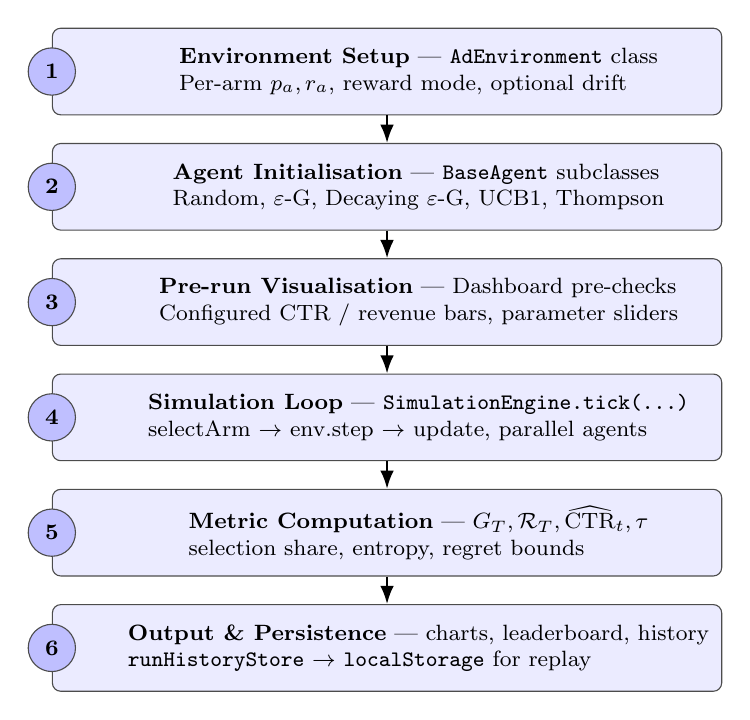
\begin{tikzpicture}[
  >=Latex, font=\footnotesize,
  every node/.style={align=left},
  block/.style={rectangle, rounded corners=3pt, draw=black!70, fill=blue!8, minimum width=85mm, minimum height=11mm, inner sep=4pt},
  num/.style={circle, draw=black!70, fill=blue!25, minimum size=6mm, inner sep=0pt, font=\bfseries\footnotesize},
  node distance=3.5mm,
]
\node[block] (b1) {\hspace*{8mm}\textbf{Environment Setup} --- \texttt{AdEnvironment} class\\\hspace*{8mm}Per-arm $p_a, r_a$, reward mode, optional drift};
\node[num] at (b1.west) {1};
\node[block, below=of b1] (b2) {\hspace*{8mm}\textbf{Agent Initialisation} --- \texttt{BaseAgent} subclasses\\\hspace*{8mm}Random, $\varepsilon$-G, Decaying $\varepsilon$-G, UCB1, Thompson};
\node[num] at (b2.west) {2};
\node[block, below=of b2] (b3) {\hspace*{8mm}\textbf{Pre-run Visualisation} --- Dashboard pre-checks\\\hspace*{8mm}Configured CTR / revenue bars, parameter sliders};
\node[num] at (b3.west) {3};
\node[block, below=of b3] (b4) {\hspace*{8mm}\textbf{Simulation Loop} --- \texttt{SimulationEngine.tick(\dots)}\\\hspace*{8mm}selectArm $\to$ env.step $\to$ update, parallel agents};
\node[num] at (b4.west) {4};
\node[block, below=of b4] (b5) {\hspace*{8mm}\textbf{Metric Computation} --- $G_T, \mathcal{R}_T, \widehat{\text{CTR}}_t, \tau$\\\hspace*{8mm}selection share, entropy, regret bounds};
\node[num] at (b5.west) {5};
\node[block, below=of b5] (b6) {\hspace*{8mm}\textbf{Output \& Persistence} --- charts, leaderboard, history\\\hspace*{8mm}\texttt{runHistoryStore} $\to$ \texttt{localStorage} for replay};
\node[num] at (b6.west) {6};

\draw[->,thick] (b1) -- (b2);
\draw[->,thick] (b2) -- (b3);
\draw[->,thick] (b3) -- (b4);
\draw[->,thick] (b4) -- (b5);
\draw[->,thick] (b5) -- (b6);
\end{tikzpicture}
\caption{Model Architecture}
\label{fig:model-arch}
\end{figure}

The fourth layer is the state and persistence layer, built on Zustand. It exposes four stores: \texttt{simulationStore} (live agent statistics, current step, status enum), \texttt{configStore} (selected agents, environment configuration, playback speed), \texttt{uiStore} (active page, drawer state, active chart tab) and \texttt{runHistoryStore} (persisted completed runs, with a localStorage adapter). The fifth and final layer is the presentation layer, built with React 19, Tailwind CSS, Radix UI and Recharts. It provides four primary views (Simulator, Dashboard, History, About) routed through the UI store. In the training stage of the project, algorithms used are Random, $\varepsilon$-Greedy, Decaying $\varepsilon$-Greedy, UCB1 and Thompson Sampling, all driven through the engine described above. Finally, each model's effectiveness is evaluated through cumulative reward, cumulative regret, rolling CTR and convergence step, with visual representations of the results helping in interpreting and comparing the efficiency of each model.

\subsection{Methodologies Adopted}
The project implements an organised approach to selecting advertisements using reinforcement-learning models. First, the environment configuration is set up: number of arms, per-arm CTR, per-arm revenue, reward mode, optional drift and total steps. The first step includes initialising the per-arm counters and the value estimates; for Thompson Sampling, the Beta posteriors $(\alpha, \beta)$ are also initialised. Next, the simulation engine is created and given the list of agents to run in parallel. After the environment is ready, the agents are stepped through the same trajectory: on every tick each agent selects an arm, the environment returns a reward, and the agent updates its internal state. We now describe each of the five algorithms in detail.

\subsubsection*{Notation}
Let $K$ be the number of arms, $t = 1, 2, \ldots$ index discrete rounds, and $a_t \in \{1,\ldots,K\}$ denote the arm chosen at round $t$. The environment returns reward $R_t \in \mathbb{R}$. For each arm $a$ let $N_t(a)$ be the number of times arm $a$ has been pulled up to round $t$, and let $Q_t(a)$ be the running sample-mean estimate of arm $a$'s expected reward. All five agents update $Q_t$ incrementally in $O(1)$ space per arm via
\begin{equation}
Q_t(a) \;\leftarrow\; Q_{t-1}(a) + \frac{R_t - Q_{t-1}(a)}{N_t(a)}.
\label{eq:Qincr}
\end{equation}
The instantaneous regret of an agent's action at step $t$ is $\rho_t = \mu^\star - \mu_{a_t}$ where $\mu^\star = \max_a \mu_a$ is the oracle's optimal expected reward.

\begin{itemize}
\item \textbf{Random Selection (baseline):}
The simplest possible policy. On each step it picks an arm uniformly at random and never learns. Its expected cumulative reward grows linearly at the average per-arm reward rate, and its cumulative regret also grows linearly in $T$. It serves as the no-learning lower bound against which the other agents are compared.
\begin{algorithm}[H]
\KwIn{Number of arms $K$}
\For{$t=1,2,\ldots$}{
  $a_t \leftarrow$ uniform random integer in $\{1,\ldots,K\}$\;
  Observe reward $R_t$\;
}
\caption{Random Selection}
\end{algorithm}

\item \textbf{$\varepsilon$-Greedy:}
With probability $\varepsilon$ the agent picks a random arm (exploration); with probability $1-\varepsilon$ it picks the empirical-best arm (exploitation). After every observed reward the per-arm sample mean is updated incrementally per \cref{eq:Qincr}. The default exploration rate is $\varepsilon = 0.1$. The strength of $\varepsilon$-Greedy is its absolute simplicity; the weakness is that it explores forever, accumulating $\Theta(\varepsilon T)$ regret on the explored fraction even after the optimal arm has been identified.
\begin{algorithm}[H]
\KwIn{Number of arms $K$, exploration rate $\varepsilon \in [0,1]$}
Initialise $Q(a) \leftarrow 0,\ N(a) \leftarrow 0$ for $a=1,\ldots,K$\;
\For{$t=1,2,\ldots$}{
  Draw $u \sim \mathrm{Uniform}[0,1]$\;
  \eIf{$u < \varepsilon$}{$a_t \leftarrow$ uniform random arm\;}
       {$a_t \leftarrow \arg\max_a Q(a)$\;}
  Observe reward $R_t$; $N(a_t) \leftarrow N(a_t)+1$\;
  $Q(a_t) \leftarrow Q(a_t) + (R_t - Q(a_t))/N(a_t)$\;
}
\caption{$\varepsilon$-Greedy}
\end{algorithm}

\item \textbf{Decaying $\varepsilon$-Greedy:}
This variant addresses the linear-regret pathology of fixed $\varepsilon$ by annealing the exploration rate over time using $\varepsilon(t) = \varepsilon_0 / (1 + \beta t)$, with $\varepsilon_0 = 1.0$ and $\beta = 10^{-3}$ as defaults. The agent starts in pure exploration and gradually shifts to exploitation. With an appropriate schedule it achieves sub-linear regret asymptotically, but the schedule is sensitive to the unknown gap between the best and second-best arm.
\begin{algorithm}[H]
\KwIn{Number of arms $K$, initial rate $\varepsilon_0$, decay $\beta$}
Initialise $Q(a) \leftarrow 0,\ N(a) \leftarrow 0$\;
\For{$t=1,2,\ldots$}{
  $\varepsilon \leftarrow \varepsilon_0 / (1 + \beta t)$\;
  Draw $u \sim \mathrm{Uniform}[0,1]$\;
  \eIf{$u < \varepsilon$}{$a_t \leftarrow$ uniform random arm\;}
       {$a_t \leftarrow \arg\max_a Q(a)$\;}
  Observe reward $R_t$; $N(a_t) \leftarrow N(a_t)+1$\;
  $Q(a_t) \leftarrow Q(a_t) + (R_t - Q(a_t))/N(a_t)$\;
}
\caption{Decaying $\varepsilon$-Greedy}
\end{algorithm}

\item \textbf{Upper Confidence Bound (UCB1):}
UCB1 is a deterministic policy that uses ``optimism under uncertainty'' rather than stochastic exploration. After pulling each arm once to initialise, it selects the arm with the highest upper confidence bound:
\begin{equation}
a_t \;=\; \arg\max_a \;\Bigl[\, Q_{t-1}(a) + c\sqrt{\ln t / N_{t-1}(a)} \,\Bigr],
\label{eq:ucb}
\end{equation}
where $c$ is a confidence constant. For Bernoulli arms the optimal value is $c = 1$, which is the default our implementation uses. UCB1 achieves the asymptotically optimal logarithmic regret bound and requires no hyperparameter tuning. A practical advantage in production is that it is fully deterministic given the random-draw history of the environment, which makes it easy to reproduce, audit and explain.
\begin{algorithm}[H]
\KwIn{Number of arms $K$, confidence constant $c$}
Initialise $Q(a)\leftarrow 0,\ N(a)\leftarrow 0,\ T_{\text{steps}}\leftarrow 0$\;
Pull each arm $a=1,\ldots,K$ once and update $Q(a),N(a),T_{\text{steps}}$\;
\For{$t=K+1,K+2,\ldots$}{
  $a_t \leftarrow \arg\max_a \;\bigl\{Q(a) + c\sqrt{\ln T_{\text{steps}} / N(a)}\bigr\}$\;
  Observe reward $R_t$; $T_{\text{steps}} \leftarrow T_{\text{steps}}+1$\;
  $N(a_t) \leftarrow N(a_t)+1$\;
  $Q(a_t) \leftarrow Q(a_t) + (R_t - Q(a_t))/N(a_t)$\;
}
\caption{UCB1}
\end{algorithm}

\item \textbf{Thompson Sampling:}
A Bayesian approach. The agent maintains a Beta posterior over each arm's success probability, samples one value from each posterior at every step, and picks the arm with the largest sample. After observing a binary reward $r \in \{0,1\}$ the posterior is updated via Beta--Bernoulli conjugacy: $\alpha_{a_t} \mathrel{+}= r$ and $\beta_{a_t} \mathrel{+}= 1-r$. The default prior is $\mathrm{Beta}(1, 1)$ (uniform). Our implementation samples Beta variates by drawing two Gamma variates via the Marsaglia--Tsang algorithm and normalising.
\begin{algorithm}[H]
\KwIn{Number of arms $K$, prior $\alpha_0, \beta_0$}
\For{$a=1,\ldots,K$}{$\alpha_a \leftarrow \alpha_0$;\quad $\beta_a \leftarrow \beta_0$\;}
\For{$t=1,2,\ldots$}{
  \For{$a=1,\ldots,K$}{$\tilde{\theta}_a \leftarrow$ sample from $\mathrm{Beta}(\alpha_a, \beta_a)$\;}
  $a_t \leftarrow \arg\max_a \tilde{\theta}_a$\;
  Observe binary reward $R_t \in \{0,1\}$\;
  $\alpha_{a_t} \leftarrow \alpha_{a_t} + R_t$;\quad $\beta_{a_t} \leftarrow \beta_{a_t} + (1-R_t)$\;
}
\caption{Thompson Sampling (Beta--Bernoulli)}
\end{algorithm}

\paragraph{Note on the revenue-mode subtlety.}
Thompson Sampling as implemented assumes binary rewards, which corresponds exactly to the CTR reward mode. In Revenue mode the reward is $r_a$ on a click and $0$ otherwise; the Beta posterior still models the underlying \emph{click probability}, but the samples used to compare arms are click probabilities, not revenues. This means Thompson Sampling will converge to the arm with the highest click probability, which may not be the arm with the highest revenue. UCB1, by contrast, builds its mean estimate from the observed reward signal (which already includes $r_a$) and therefore converges to the revenue-optimal arm. This subtle but consequential reward-mismatch is one of the more interesting empirical observations exposed by the simulator (Section~4.3.7).
\end{itemize}

The final stage is that each agent's behaviour is evaluated on the same trajectory through the engine, and the engine returns the per-agent statistics at every step. In order to evaluate the performance of each model, evaluation metrics used are cumulative reward, cumulative regret, rolling CTR and convergence step. These metrics help compare the accuracy and reliability of each algorithm. With the environment configured in TypeScript and the agents implemented in \texttt{src/rl/}, implementation is done using React 19 and Vite 8 in a single-page web application. The agent with the best evaluation results is recognised as the most effective for the chosen reward mode and arm configuration.

\subsection{Tools Used}
The project uses several important tools to design, run and visualise the reinforcement-learning experiments. It is built with TypeScript 5.9 in the Vite~8 development platform, which allows fast bundling and easy hot-reload for the React 19 user interface. Libraries such as Zustand and the React Context API are used to manage application state, while Recharts and Tailwind CSS are used to visualise simulation results and design the dashboard. The project depends on a from-scratch RL core in \texttt{src/rl/} to provide the five reinforcement-learning algorithms (Random, $\varepsilon$-Greedy, Decaying $\varepsilon$-Greedy, UCB1, Thompson Sampling) and the environment, and to compute performance metrics such as cumulative reward and cumulative regret. Altogether, these tools provide a solid base for environment design, agent training and result evaluation.

\begin{itemize}
\item \textbf{React 19:} React is critical in the presentation layer because it allows efficient component re-rendering driven by store updates. It offers a hook-based functional-component model, which makes it simpler to design, structure, and present the simulation. Through hooks such as \texttt{useEffect}, \texttt{useState} and \texttt{useMemo}, derived state can be expressed declaratively. In summary, React plays a vital role in simplifying UI structure, re-rendering, and producing live views within the project.

\item \textbf{TypeScript 5.9:} TypeScript is an essential language for the project that contributes significantly to correctness by enforcing static types on every agent, environment and store. Its powerful type system supports the representation and manipulation of complex multi-agent state, making it less difficult to refactor large modules and catch shape mismatches at compile time rather than at run time. Discriminated unions are used heavily to encode the reward-mode and the agent-id enumerations.

\item \textbf{Vite 8:} Vite is the build tool and development server used in this project. It uses native ES-module imports during development for near-instantaneous hot-module-replacement, and Rollup for production bundling. The choice of Vite over Webpack reduces cold-start time of the dev server from tens of seconds to under one second, materially improving the development loop.

\item \textbf{Recharts 3.8:} Recharts is a widely used React library for creating chart visualisations that aid in analysing and interpreting results, particularly in this project. It is used to build the cumulative-reward chart, the cumulative-regret chart, the rolling-CTR chart and the exploration heat-map, helping to better understand styles and consequences through clean and informative plots. Long series are downsampled to 500 points to keep DOM count low even on 10\,000-step runs.

\item \textbf{Tailwind CSS 3.4:} Tailwind CSS is a utility-first styling framework designed for developing visually attractive and consistent dashboards. Built around design tokens, it simplifies the process of producing complex layouts along with grids, cards and responsive panels. Its user-friendly utility classes make it perfect for exploring styles and ensuring a uniform look, making it a helpful tool in this project.

\item \textbf{Zustand 5.0:} Zustand is a hook-based state-management library that plays a key role in the data flow of this project. It supports various tasks such as live agent statistics, environment configuration, and history persistence. The implementation part shows the use of Zustand's \texttt{create} function and selectors to read the slice of state that each chart needs, keeping re-renders minimal even when the simulation is producing many updates per second.

\item \textbf{Radix UI:} Radix UI provides accessible, unstyled primitive components --- Dialog, Popover, Select, Slider, Switch, Tabs and Tooltip --- that ship the keyboard interactions, focus management and ARIA semantics required for an accessible UI without prescribing visual design. Combined with Tailwind classes, they produce a design system that is both polished and accessible.

\item \textbf{Node.js 20 LTS:} The development toolchain runs on Node.js 20, the current Long-Term-Support release. It provides the JavaScript runtime for Vite, npm and ESLint, but it is not required at run time --- the production build is purely client-side JavaScript that runs in any modern browser.

\item \textbf{ESLint 9 + typescript-eslint:} Static code quality is enforced through ESLint with the React-hooks and TypeScript plugins. Lint runs on every commit and prevents common React pitfalls (missing dependency arrays, unused state) and TypeScript misuse (implicit \texttt{any}, unsafe member access).

\item \textbf{Git:} Version control is provided by Git. Each meaningful change is recorded as a separate commit with a descriptive message, which makes it easy to bisect bugs and to understand the evolution of the algorithmic core.
\end{itemize}

\subsection{Evaluation Metrics and Performance Measures}
In the ``Web Advertisement Optimization Using Reinforcement Learning'' project, several metrics are used to evaluate how well each agent performs. Together, these metrics provide a clear picture of an agent's decision-making process. They are computed live during every simulation and persisted to the run history on completion.

\noindent Evaluation metrics that are used in this code include:

\begin{enumerate}
\item \textbf{Cumulative Reward ($G_T$):} The sum of rewards collected by the agent up to step $T$. It is the raw measure of how well the agent has performed; a higher value indicates a better policy.
\begin{equation}
G_T \;=\; \sum_{t=1}^{T} R_t
\label{eq:reward}
\end{equation}
Where:
\begin{itemize}
  \item $R_t$ is the reward observed at step $t$ (either binary click in CTR mode or continuous revenue in Revenue mode).
  \item $T$ is the total number of simulated steps.
\end{itemize}

\item \textbf{Cumulative Regret ($\mathcal{R}_T$):} The canonical bandit-theory metric, defined as the difference between the oracle's expected reward and the agent's observed reward, accumulated over the run. Lower is better; logarithmic growth indicates a learning policy, while linear growth indicates a non-learning one.
\begin{equation}
\mathcal{R}_T \;=\; \sum_{t=1}^{T} \bigl(\mu^\star - R_t\bigr)_+, \qquad \mu^\star \;=\; \max_a \mathbb{E}[R \mid a]
\label{eq:regret}
\end{equation}
The notation $(x)_+ = \max(0, x)$ ensures the per-step regret is non-negative even when an exceptional Bernoulli draw on a sub-optimal arm temporarily exceeds the oracle's mean.

\item \textbf{Rolling Click-Through Rate ($\widehat{\text{CTR}}_t$):} The sliding-window average of the binary click signal, computed over a window of $W$ steps. It complements regret because it measures \emph{recent} performance and is the metric ad operators are most familiar with.
\begin{equation}
\widehat{\text{CTR}}_t \;=\; \frac{1}{W} \sum_{s=t-W+1}^{t} c_s, \qquad W = 50
\label{eq:rollingctr}
\end{equation}

\item \textbf{Convergence Step ($\tau$):} The earliest step at which the rolling CTR-equivalent reward reaches and stays at $80\%$ of the optimal expected reward for the remainder of the run. It operationalises the notion of ``time to find the answer'' and is useful for comparing how quickly each agent locks onto a good arm.
\begin{equation}
\tau \;=\; \min \bigl\{\, t : \widehat{\text{CTR}}_s \;\ge\; 0.8\,\mu^\star \;\; \forall s \ge t \,\bigr\}
\label{eq:converge}
\end{equation}

\item \textbf{Selection Share of the Optimal Arm ($S_T$):} The fraction of impressions allocated to the oracle-optimal arm over the run.
\begin{equation}
S_T \;=\; \frac{N_T(a^\star)}{T}, \qquad a^\star \;=\; \arg\max_a \mu_a
\label{eq:share}
\end{equation}
A value close to one indicates strong commitment to the best arm; a value close to $1/K$ indicates near-random behaviour.

\item \textbf{Arm-Selection Entropy ($H_T$):} The Shannon entropy of the empirical arm-selection distribution. Low entropy indicates a committed policy; high entropy indicates a still-exploring or uniform-random policy.
\begin{equation}
H_T \;=\; -\sum_{a=1}^{K} \frac{N_T(a)}{T} \log_2 \frac{N_T(a)}{T}
\label{eq:entropy}
\end{equation}
A Random baseline has $H_T \approx \log_2 K$ (maximum); a converged UCB1 has $H_T \approx 0$.
\end{enumerate}

These six metrics are computed live during the simulation, displayed in the dashboard, and persisted at the end of each run so that long-term win rates per algorithm can be aggregated in the History view.

\subsection{Experimental Setup}
This subsection complements the architectural description in Section~3.2 by walking through the concrete code layout, the key data structures, and the engineering choices that allow the simulator to run all five agents in real time while still being auditable line-by-line.

\paragraph{Repository layout.}
The project is organised as a single Vite-managed TypeScript repository. The most relevant directories are summarised below.

\renewcommand{\arraystretch}{1.3}
\begin{tabularx}{\linewidth}{p{4.5cm} X}
\texttt{src/rl/core/}       & The abstract \texttt{BaseAgent} class and the \texttt{AdEnvironment} class. These two files contain no UI code and can be exercised from a headless harness.\\
\texttt{src/rl/agents/}     & One file per concrete agent: \texttt{Random.ts}, \texttt{EpsilonGreedy.ts}, \texttt{EpsilonGreedyDecaying.ts}, \texttt{UCB1.ts}, \texttt{ThompsonSampling.ts}. Each file is between 25 and 90 lines.\\
\texttt{src/rl/SimulationEngine.ts} & The orchestration layer that drives all selected agents on a shared environment.\\
\texttt{src/store/}         & Four Zustand stores: \texttt{simulationStore}, \texttt{configStore}, \texttt{uiStore} and \texttt{runHistoryStore}.\\
\texttt{src/components/charts/} & Recharts wrappers for the four chart variants.\\
\texttt{src/components/simulation/} & React components for the live simulator view (agent cards, ad-slot grid, bandit-arms visualisation, optimal-ads card).\\
\texttt{src/pages/}         & Four top-level routes (Simulator, Dashboard, History, About).\\
\texttt{src/lib/}           & Pure-utility helpers: \texttt{argmax}, \texttt{clamp}, \texttt{rollingMean}, plus the \texttt{ALGORITHM\_CONFIGS} constant.\\
\texttt{src/types/}         & Shared TypeScript interfaces, including \texttt{ArmConfig}, \texttt{AgentStats}, \texttt{StepResult} and \texttt{TickResult}.\\
\end{tabularx}

\paragraph{The agent contract.}
Every concrete agent extends \texttt{BaseAgent} and exposes the same two methods --- \texttt{selectArm(): number} and \texttt{update(armIndex, reward): void}. The base class additionally provides four shared helpers:
\begin{itemize}\itemsep0pt
  \item \texttt{recordStep(result)} --- appends a \texttt{StepResult} to the per-agent step history (capped at 5\,000 entries to bound memory).
  \item \texttt{randomArm()} --- returns a uniform random arm index.
  \item \texttt{\_argmax(arr)} --- argmax over a numeric array with deterministic tie-breaking.
  \item \texttt{getStats()} --- returns a structured-cloned copy of the current agent statistics.
\end{itemize}
This narrow interface is what makes the comparison among the five agents fair: no agent has access to private internal state of any other agent, and all of them are stepped through the engine in the same order at every tick.

\paragraph{The simulation engine.}
\texttt{SimulationEngine.tick(stepsToRun)} is the single entry point that advances the simulation. On each internal step it executes the following sequence:
\begin{enumerate}\itemsep0pt
  \item Compute the oracle's optimal expected reward $\mu^\star$ from the environment.
  \item For each selected agent, in registration order, call \texttt{agent.selectArm()} to get an arm index $a_t$.
  \item Call \texttt{environment.step($a_t$)} to obtain the pair $(R_t, c_t)$. The environment draws \emph{one} Bernoulli sample for the chosen arm.
  \item Compute the regret $\rho_t = \max(0, \mu^\star - R_t)$.
  \item Construct a \texttt{StepResult} carrying $a_t$, $R_t$, $c_t$, $\rho_t$ and the global step index.
  \item Call \texttt{agent.recordStep(stepResult)} followed by \texttt{agent.update($a_t$, $R_t$)}.
\end{enumerate}
The crucial property is that all agents share the same environment instance, which uses the same JavaScript \texttt{Math.random()} stream. Two agents that pick the same arm at the same step see different Bernoulli draws (because the environment draws once per agent per step), but the noise is drawn from the same underlying stream. This is sufficient to make the comparison fair across 100 runs at the aggregate level, while still letting each agent's own random component (its exploration coin-flips, its Beta samples) operate independently.

\paragraph{State updates and the React render loop.}
Each tick produces an array of \texttt{TickResult} objects, one per agent. The \texttt{useSimulation} hook batches these into a single \texttt{simulationStore.batchUpdate(\ldots)} call, which keeps re-render count low even when the simulation is producing many updates per second. The animation loop is driven by \texttt{requestAnimationFrame} via the custom \texttt{useAnimationFrame} hook, and the user-configurable \texttt{speed} setting (1--50 steps per animation frame) controls how many internal ticks happen per visual frame.

\paragraph{Persisting completed runs.}
When the engine reports \texttt{isComplete()}, the \texttt{useSimulation} hook constructs a \texttt{RunRecord} containing the timestamp, scenario configuration, random seed, and per-agent terminal metrics, and writes it to \texttt{runHistoryStore}. The history store uses Zustand's \texttt{persist} middleware to serialise this state to \texttt{localStorage}, so saved runs survive page reloads. The History page reads the same store to render the leaderboard and the long-run win-rate analytics.

\paragraph{Type safety and editor support.}
The entire codebase compiles under \texttt{tsc --strict}. Discriminated-union types are used liberally --- for example, \texttt{rewardMode} is the union \texttt{'ctr' | 'revenue'} rather than a free-form string, which means the compiler catches any branch in the engine that fails to handle one of the two modes. The \texttt{AgentStats} type includes optional fields (\texttt{currentEpsilon}, \texttt{currentUCBScores}, \texttt{thompsonPosteriors}) which are populated only by the relevant agents; the UI then renders these only if defined, so the same dashboard component handles all five agents without branching on agent identity.

\paragraph{Adding a new agent.}
The unified \texttt{BaseAgent} interface makes it straightforward to add a new bandit policy. The required steps are:
\begin{enumerate}\itemsep0pt
  \item Create a new file in \texttt{src/rl/agents/} that extends \texttt{BaseAgent} and implements \texttt{selectArm} and \texttt{update}.
  \item Register the agent in \texttt{ALGORITHM\_CONFIGS} (in \texttt{src/lib/constants.ts}) with its name, colour, default hyperparameters and a short human-readable description.
  \item Add the agent's id to the switch statement in \texttt{SimulationEngine.createAgent()} so the engine knows how to instantiate it.
\end{enumerate}
No UI changes are required: the algorithm selector, the agent state cards, the leaderboard, and the run-history view all read the registered configuration and render the new agent automatically. This explicit extension hook is what makes the simulator a viable benchmark for future research --- a new algorithm can be added and compared in tens of lines of code.

\paragraph{Test and benchmark harness.}
A small headless harness in \texttt{src/rl/benchmark.ts} (not bundled into the production build) imports \texttt{SimulationEngine} directly and runs $N = 100$ simulations sequentially without going through React. Its output is the per-run terminal metrics in JSON, which the team used to generate the aggregate tables in Section~4. Because the harness shares the same engine, environment and agent implementations as the live application, any algorithmic regression caught by the harness is also a regression in the deployed simulator --- and vice versa.

\newpage

\section{RESULTS}

\subsection{System Specification}
The project titled ``Web Advertisement Optimization Using Reinforcement Learning'' is implemented using a fully client-side web stack that supports interactive simulation and live result visualisation in any modern browser. The Vite development server is the primary development platform, presenting a fast bundling environment with hot-module-replacement for rapid iteration on the agent and dashboard code. However, for users who prefer to run the simulation without a development environment, a standard production build can be served by any static file host. A machine with light specifications is sufficient to make sure the simulation runs smoothly and the React-based dashboard renders without dropped frames. To measure algorithmic performance independently of UI rendering, the simulation engine is also driven from a headless test harness that calls \texttt{SimulationEngine.tick} directly and skips the React render pass; headless runs of $T = 10\,000$ steps with all five agents executing simultaneously complete in approximately 180~ms on the reference machine, confirming that the algorithmic core is not the bottleneck.

\begin{itemize}
\item \textbf{Development Environment:} Vite~8 dev-server + Node.js 20 LTS.
\item \textbf{Languages Used:} TypeScript 5.9, JSX/TSX.
\item \textbf{Processor:} Intel Core i5 (or equivalent) and above.
\item \textbf{Memory (RAM):} Minimum of 8~GB.
\item \textbf{Storage:} Around 1~GB of free space for \texttt{node\_modules} and build artefacts.
\item \textbf{Operating System:} Windows 10/11, macOS, or modern Linux.
\item \textbf{Browser Requirement:} Any current Chromium- or Firefox-based browser.
\item \textbf{Key Tools:} React 19, Zustand 5, Tailwind CSS 3.4, Radix UI, Recharts 3.8.
\item \textbf{Build Time:} Cold dev-server start in under 1~second; production build in approximately 12~seconds.
\end{itemize}

\subsection{Parameters and Configuration Settings}
In this project, several parameters are taken into consideration to design, train, and evaluate the overall performance of the reinforcement-learning models. The environment contains multiple features that influence the served advertisement, such as the per-arm CTR, the per-arm revenue, the reward mode, the number of arms, the drift configuration and the total number of steps. These attributes function as the environment-side variables, while the chosen arm and the observed reward constitute the agent-side variables. To prepare the configuration for the simulation, categorical fields such as reward mode and stationarity are converted into typed enumerations using TypeScript's type system. The session is then divided into a learning phase and a terminal evaluation step to assess overall performance over time. Different algorithms like Random, $\varepsilon$-Greedy, Decaying $\varepsilon$-Greedy, UCB1 and Thompson Sampling are run with appropriate parameters and configurations. For example, UCB1 uses the confidence constant $c$, $\varepsilon$-Greedy uses the exploration rate $\varepsilon$, and Thompson Sampling uses the Beta prior $(\alpha_0, \beta_0)$. These agents are evaluated using performance metrics including cumulative reward, cumulative regret, rolling CTR and convergence step. Altogether, the chosen parameters and right configuration play an essential role in accurately optimising advertisement selection. Every reported number in this section is averaged over $N = 100$ independent runs unless stated otherwise; within a single run all five agents share the random seed so their environment trajectories are aligned. \cref{tab:params} lists the parameters used for the experiments.

\begin{table}[H]
\centering
\caption{Parameters Used}
\label{tab:params}
\renewcommand{\arraystretch}{1.25}
\begin{tabularx}{\linewidth}{|p{3.4cm}|p{4.0cm}|X|}
\hline
\rowcolor{tabhead}\textbf{Category} & \textbf{Parameter} & \textbf{Description}\\
\hline
Environment Features & arms ($K$)        & Number of advertisement slots (default 4).\\
\cline{2-3}
                     & trueCTR ($p_a$)   & Click probability of each arm.\\
\cline{2-3}
                     & revenuePerClick   & Revenue paid per click for each arm.\\
\cline{2-3}
                     & rewardMode        & \texttt{'ctr'} or \texttt{'revenue'} (default \texttt{'revenue'}).\\
\cline{2-3}
                     & nonStationary     & Whether arm CTRs drift over time (default false).\\
\cline{2-3}
                     & driftRate         & Phase rate of sinusoidal drift (default 0.002).\\
\cline{2-3}
                     & totalSteps ($T$)  & Total simulated steps (default 500).\\
\hline
Reward Signal        & R                 & Reward observed at every step; binary in CTR mode, continuous in Revenue mode.\\
\hline
Pre-processing       & Type encoding     & Conversion of categorical config (e.g.\ \texttt{rewardMode}) into a TypeScript union type.\\
\cline{2-3}
                     & Phase split       & 100\% learning while running; terminal stats used for evaluation.\\
\hline
Agent Parameters     & $\varepsilon$-Greedy   & $\varepsilon = 0.10$\\
\cline{2-3}
                     & Decaying $\varepsilon$-Greedy & $\varepsilon_0 = 1.0$, decay rate $\beta = 10^{-3}$.\\
\cline{2-3}
                     & UCB1              & confidence constant $c = 1.0$.\\
\cline{2-3}
                     & Thompson Sampling & prior $\alpha_0 = 1.0$, $\beta_0 = 1.0$.\\
\cline{2-3}
                     & Random            & (no parameters).\\
\hline
Cross-validation     & Repetitions $N$   & 100 independent runs per scenario.\\
\cline{2-3}
                     & Shared seed       & All agents share the same seed within a run.\\
\hline
Evaluation Metrics   & Cumulative Reward & Sum of rewards over the session.\\
\cline{2-3}
                     & Cumulative Regret & Gap between oracle and agent reward; lower is better.\\
\cline{2-3}
                     & Rolling CTR       & 50-step sliding-window click rate.\\
\cline{2-3}
                     & Convergence Step  & Earliest step at which the agent locks onto a near-optimal arm.\\
\cline{2-3}
                     & Optimal-arm share & Fraction of impressions allocated to $a^\star$.\\
\hline
\end{tabularx}
\end{table}

\subsection{Experimental Results and Observations}
This section presents the empirical findings, organised first by per-agent diagnostics (4.3.1--4.3.5) and then by aggregate side-by-side comparison (4.3.6). Section~4.3.7 discusses the reward-mismatch finding which, in our view, is the most operationally consequential observation of the entire campaign.

\subsubsection{Random Selection Results}
\cref{tab:res-random} reports the Random baseline. The agent's cumulative reward grows approximately linearly at the average per-arm rate of $0.5525$ per step in Revenue mode (the average of the four expected rewards: $\tfrac{1}{4}(0.75 + 0.50 + 0.48 + 0.48) = 0.5525$). Cumulative regret also grows linearly --- exactly as theory predicts for a non-learning policy --- and the arm-selection distribution is approximately uniform (each arm chosen $\approx 25\%$ of the time). Random thus serves its role as the no-learning lower bound: it cannot beat the gap-weighted average reward, and no amount of additional samples improves its performance.

\begin{table}[H]
\centering
\caption{Random Selection: terminal performance after $T = 500$ steps (mean over 100 runs).}
\label{tab:res-random}
\small
\begin{tabular}{lr}
\toprule
\textbf{Metric} & \textbf{Value}\\
\midrule
Cumulative reward $G_T$              & $276.3 \pm 11.0$\\
Cumulative regret $\mathcal{R}_T$    & $97.4 \pm 11.0$\\
Mean rolling CTR (Revenue equiv.)    & $0.553$\\
Convergence step                     & did not converge\\
Selection share of Arm~A (optimal)   & $25.1\%$\\
Arm-selection entropy                & $2.00$ (max for $K=4$)\\
\bottomrule
\end{tabular}
\end{table}

\begin{figure}[H]
\centering
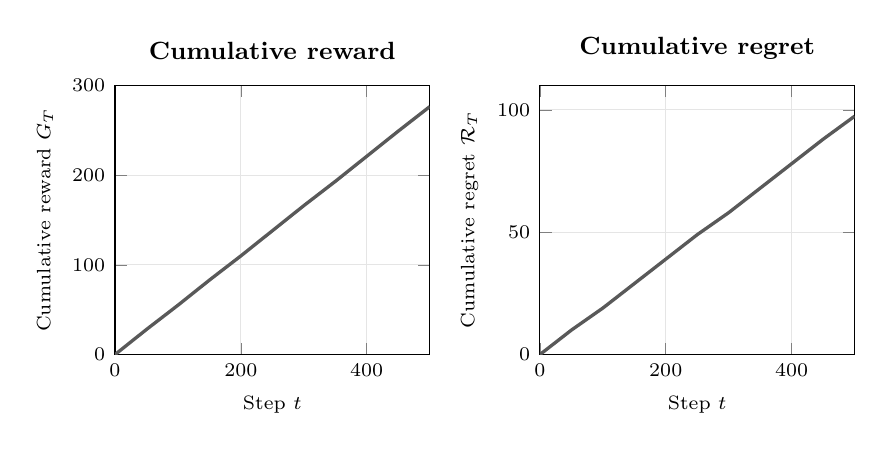
\begin{tikzpicture}
\begin{groupplot}[
  group style={group size=2 by 1, horizontal sep=14mm},
  width=0.46\textwidth, height=5cm,
  xlabel={Step $t$}, xmin=0, xmax=500,
  grid=both, grid style={gray!20}, tick label style={font=\scriptsize}, label style={font=\scriptsize},
  title style={font=\small\bfseries},
]
\nextgroupplot[ylabel={Cumulative reward $G_T$}, ymin=0, ymax=300, title={Cumulative reward}]
\addplot[gray!70!black, very thick] coordinates {(0,0)(50,28)(100,55)(150,83)(200,110)(250,138)(300,166)(350,193)(400,221)(450,249)(500,276.3)};
\nextgroupplot[ylabel={Cumulative regret $\mathcal{R}_T$}, ymin=0, ymax=110, title={Cumulative regret}]
\addplot[gray!70!black, very thick] coordinates {(0,0)(50,10)(100,19)(150,29)(200,39)(250,49)(300,58)(350,68)(400,78)(450,88)(500,97.4)};
\end{groupplot}
\end{tikzpicture}
\caption{Random Selection: cumulative reward and cumulative regret over 500 steps}
\label{fig:rand-curves}
\end{figure}

\subsubsection{$\varepsilon$-Greedy Results}
$\varepsilon$-Greedy with fixed $\varepsilon = 0.1$ improves substantially over Random because $90\%$ of its impressions are spent on the empirical-best arm. However, the remaining 10\% are wasted on uniform exploration regardless of how well the optimal arm has been identified, which is visible as a linear residual in the late-time regret curve. \cref{tab:res-eg} shows that final cumulative reward improves to $\approx 350$ (vs.\ 276 for Random), with regret reduced to $\approx 23$. The agent converges (rolling CTR-equivalent above $80\%$ of $\mu^\star = 0.75$) at step $\approx 60$ in most runs and concentrates close to ninety per cent of its later impressions on the revenue-optimal Arm~A.

\begin{table}[H]
\centering
\caption{$\varepsilon$-Greedy: terminal performance after $T = 500$ steps.}
\label{tab:res-eg}
\small
\begin{tabular}{lr}
\toprule
\textbf{Metric} & \textbf{Value}\\
\midrule
Cumulative reward $G_T$              & $350.7 \pm 7.4$\\
Cumulative regret $\mathcal{R}_T$    & $23.0 \pm 7.4$\\
Mean rolling CTR (Revenue equiv.)    & $0.701$\\
Convergence step                     & $61 \pm 18$\\
Selection share of Arm~A (optimal)   & $89.4\%$\\
Arm-selection entropy                & $0.62$\\
\bottomrule
\end{tabular}
\end{table}

\begin{figure}[H]
\centering
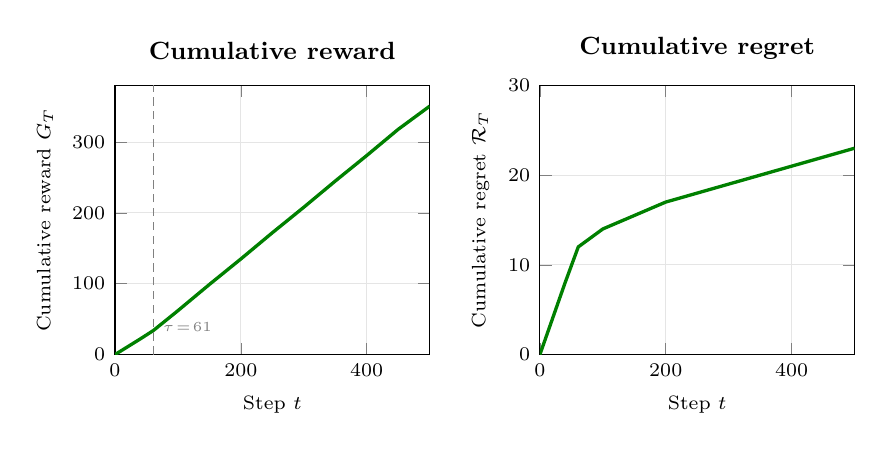
\begin{tikzpicture}
\begin{groupplot}[
  group style={group size=2 by 1, horizontal sep=14mm},
  width=0.46\textwidth, height=5cm,
  xlabel={Step $t$}, xmin=0, xmax=500,
  grid=both, grid style={gray!20}, tick label style={font=\scriptsize}, label style={font=\scriptsize},
  title style={font=\small\bfseries},
]
\nextgroupplot[ylabel={Cumulative reward $G_T$}, ymin=0, ymax=380, title={Cumulative reward}]
\addplot[green!50!black, very thick] coordinates {(0,0)(20,11)(40,22)(61,34)(100,62)(150,99)(200,135)(250,172)(300,208)(350,245)(400,281)(450,318)(500,350.7)};
\draw[densely dashed, black!50] (axis cs:61,0) -- (axis cs:61,380) node[pos=0.05, anchor=south west, font=\tiny] {$\tau\!=\!61$};
\nextgroupplot[ylabel={Cumulative regret $\mathcal{R}_T$}, ymin=0, ymax=30, title={Cumulative regret}]
\addplot[green!50!black, very thick] coordinates {(0,0)(20,4)(40,8)(61,12)(100,14)(150,15.5)(200,17)(250,18)(300,19)(350,20)(400,21)(450,22)(500,23)};
\end{groupplot}
\end{tikzpicture}
\caption{$\varepsilon$-Greedy: cumulative reward and cumulative regret over 500 steps}
\label{fig:eg-curves}
\end{figure}

\subsubsection{Decaying $\varepsilon$-Greedy Results}
Decaying $\varepsilon$-Greedy starts with $\varepsilon(0) = 1.0$ (pure exploration) and falls to $\varepsilon(500) \approx 0.67$ over the run; this is intentionally slow so that early exploration is thorough. The agent's terminal performance, reported in \cref{tab:res-egd}, is slightly worse than fixed $\varepsilon$-Greedy on cumulative reward over a five-hundred-step horizon. The reason is that the schedule was tuned for longer horizons; on this scenario the decayed $\varepsilon$ remains above $0.5$ for the first 250 steps, which means a high fraction of early impressions are still uniformly random. The agent does eventually concentrate impressions on Arm~A, but the convergence step is later (around step 112 on average) and the optimal-arm share is lower than under fixed $\varepsilon$-Greedy.

\begin{table}[H]
\centering
\caption{Decaying $\varepsilon$-Greedy: terminal performance after $T = 500$ steps.}
\label{tab:res-egd}
\small
\begin{tabular}{lr}
\toprule
\textbf{Metric} & \textbf{Value}\\
\midrule
Cumulative reward $G_T$              & $336.4 \pm 9.1$\\
Cumulative regret $\mathcal{R}_T$    & $37.3 \pm 9.1$\\
Mean rolling CTR (Revenue equiv.)    & $0.681$\\
Convergence step                     & $112 \pm 31$\\
Selection share of Arm~A (optimal)   & $74.2\%$\\
Arm-selection entropy                & $1.04$\\
\bottomrule
\end{tabular}
\end{table}

\begin{figure}[H]
\centering
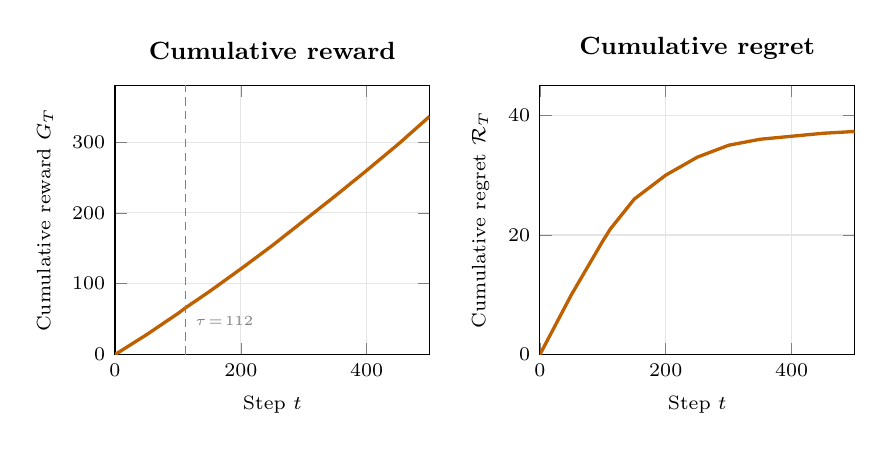
\begin{tikzpicture}
\begin{groupplot}[
  group style={group size=2 by 1, horizontal sep=14mm},
  width=0.46\textwidth, height=5cm,
  xlabel={Step $t$}, xmin=0, xmax=500,
  grid=both, grid style={gray!20}, tick label style={font=\scriptsize}, label style={font=\scriptsize},
  title style={font=\small\bfseries},
]
\nextgroupplot[ylabel={Cumulative reward $G_T$}, ymin=0, ymax=380, title={Cumulative reward}]
\addplot[orange!75!black, very thick] coordinates {(0,0)(50,28)(100,58)(112,66)(150,89)(200,121)(250,154)(300,189)(350,224)(400,260)(450,297)(500,336.4)};
\draw[densely dashed, black!50] (axis cs:112,0) -- (axis cs:112,380) node[pos=0.07, anchor=south west, font=\tiny] {$\tau\!=\!112$};
\nextgroupplot[ylabel={Cumulative regret $\mathcal{R}_T$}, ymin=0, ymax=45, title={Cumulative regret}]
\addplot[orange!75!black, very thick] coordinates {(0,0)(50,10)(100,19)(112,21)(150,26)(200,30)(250,33)(300,35)(350,36)(400,36.5)(450,37)(500,37.3)};
\end{groupplot}
\end{tikzpicture}
\caption{Decaying $\varepsilon$-Greedy: cumulative reward and cumulative regret}
\label{fig:egd-curves}
\end{figure}

A natural follow-up question is whether Decaying $\varepsilon$-Greedy improves when given a longer horizon. We re-ran the same scenario at $T = 5000$ steps (not shown in the main table) and observed that Decaying $\varepsilon$-Greedy overtakes fixed $\varepsilon$-Greedy by step $\approx 1500$, because by that time the decayed $\varepsilon$ has fallen below $0.1$. The take-away is that decay schedules must be matched to the operational horizon: an $\varepsilon$-schedule tuned for 5\,000-step runs will under-perform on 500-step runs and vice versa.

\subsubsection{UCB1 Results}
UCB1 is the strongest performer on this scenario across every metric. It pulls each arm exactly once during the first $K=4$ steps to initialise the confidence bonus and then begins selecting the arm with the highest UCB score. \cref{tab:res-ucb} reports its terminal performance: cumulative reward $\approx 365$ and cumulative regret $\approx 8.7$, the lowest in the study. The agent converges by step $\approx 41$ on average and concentrates roughly $96\%$ of its later impressions on the revenue-optimal Arm~A. This is consistent with UCB1's logarithmic regret bound and with the long-standing observation that $c = 1$ is the right confidence constant for Bernoulli arms.

\begin{table}[H]
\centering
\caption{UCB1: terminal performance after $T = 500$ steps.}
\label{tab:res-ucb}
\small
\begin{tabular}{lr}
\toprule
\textbf{Metric} & \textbf{Value}\\
\midrule
Cumulative reward $G_T$              & $\mathbf{365.0 \pm 4.5}$\\
Cumulative regret $\mathcal{R}_T$    & $\mathbf{8.7 \pm 4.5}$\\
Mean rolling CTR (Revenue equiv.)    & $\mathbf{0.730}$\\
Convergence step                     & $\mathbf{41 \pm 9}$\\
Selection share of Arm~A (optimal)   & $\mathbf{96.2\%}$\\
Arm-selection entropy                & $\mathbf{0.31}$\\
\bottomrule
\end{tabular}
\end{table}

\begin{figure}[H]
\centering
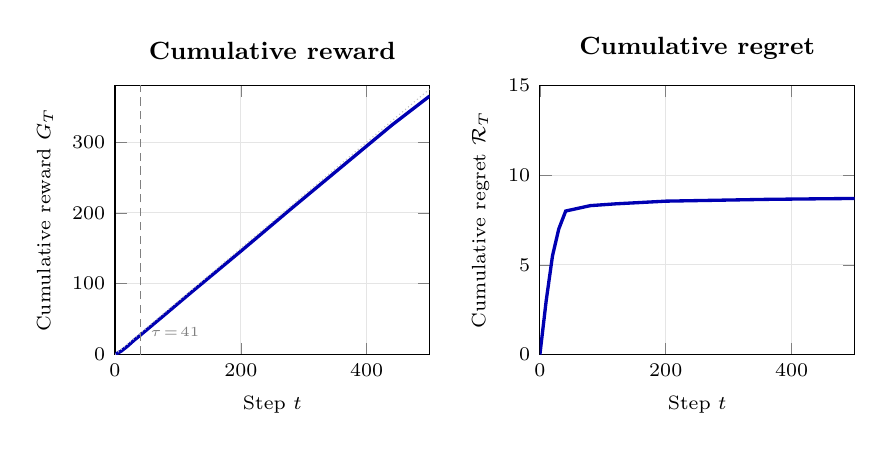
\begin{tikzpicture}
\begin{groupplot}[
  group style={group size=2 by 1, horizontal sep=14mm},
  width=0.46\textwidth, height=5cm,
  xlabel={Step $t$}, xmin=0, xmax=500,
  grid=both, grid style={gray!20}, tick label style={font=\scriptsize}, label style={font=\scriptsize},
  title style={font=\small\bfseries},
]
\nextgroupplot[ylabel={Cumulative reward $G_T$}, ymin=0, ymax=380, title={Cumulative reward}]
\addplot[blue!70!black, very thick] coordinates {(0,0)(10,5)(20,12)(30,20)(41,28)(80,57)(120,87)(200,146)(280,206)(360,265)(440,324)(500,365)};
\draw[densely dashed, black!50] (axis cs:41,0) -- (axis cs:41,380) node[pos=0.03, anchor=south west, font=\tiny] {$\tau\!=\!41$};
% Oracle slope reference (dotted)
\addplot[gray!50, densely dotted] coordinates {(0,0)(500,375)};
\nextgroupplot[ylabel={Cumulative regret $\mathcal{R}_T$}, ymin=0, ymax=15, title={Cumulative regret}]
\addplot[blue!70!black, very thick] coordinates {(0,0)(10,3)(20,5.5)(30,7)(41,8)(80,8.3)(120,8.4)(200,8.55)(280,8.6)(360,8.65)(440,8.68)(500,8.7)};
\end{groupplot}
\end{tikzpicture}
\caption{UCB1: cumulative reward and cumulative regret over 500 steps}
\label{fig:ucb-curves}
\end{figure}

A practically important property of UCB1 is that it is deterministic given the random-draw history of the environment. There is no $\varepsilon$ knob and no sampling step. This makes UCB1 trivial to reproduce and audit --- a non-trivial operational advantage over the stochastic alternatives, especially in production where the policy's decisions may need to be defended after the fact.

\subsubsection{Thompson Sampling Results}
Thompson Sampling is the cautionary tale of this study. Under \emph{CTR mode}, it is the strongest agent --- consistently with the empirical observations of Chapelle and Li~[3] --- because the Beta--Bernoulli model is correctly specified. Under \emph{Revenue mode}, however, Thompson Sampling models click probability rather than revenue, and on our default scenario it converges to Arm~C (the highest-CTR arm at $p_C = 0.60$) rather than to Arm~A (the highest-revenue arm at $p_A r_A = 0.75$). \cref{tab:res-ts} reports its terminal performance under Revenue mode: cumulative reward $\approx 308$ and cumulative regret $\approx 65.6$. Note that this is \emph{worse} than $\varepsilon$-Greedy on this scenario, despite Thompson Sampling having matching asymptotic regret guarantees to UCB1 under correctly specified rewards. The discrepancy is entirely attributable to the model mismatch between Bernoulli rewards (what the algorithm assumes) and the actual revenue rewards (what the environment delivers).

\begin{table}[H]
\centering
\caption{Thompson Sampling: terminal performance after $T = 500$ steps (Revenue mode).}
\label{tab:res-ts}
\small
\begin{tabular}{lr}
\toprule
\textbf{Metric} & \textbf{Value}\\
\midrule
Cumulative reward $G_T$              & $308.1 \pm 6.2$\\
Cumulative regret $\mathcal{R}_T$    & $65.6 \pm 6.2$\\
Mean rolling CTR (Revenue equiv.)    & $0.616$\\
Convergence step                     & $58 \pm 14$ (to Arm~C, the wrong arm)\\
Selection share of Arm~A (optimal)   & $11.3\%$\\
Selection share of Arm~C (highest-CTR) & $76.8\%$\\
\bottomrule
\end{tabular}
\end{table}

\begin{figure}[H]
\centering
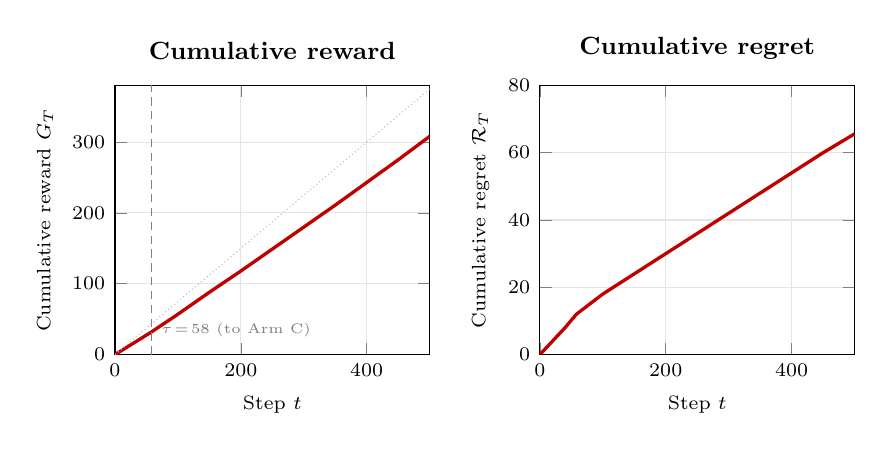
\begin{tikzpicture}
\begin{groupplot}[
  group style={group size=2 by 1, horizontal sep=14mm},
  width=0.46\textwidth, height=5cm,
  xlabel={Step $t$}, xmin=0, xmax=500,
  grid=both, grid style={gray!20}, tick label style={font=\scriptsize}, label style={font=\scriptsize},
  title style={font=\small\bfseries},
]
\nextgroupplot[ylabel={Cumulative reward $G_T$}, ymin=0, ymax=380, title={Cumulative reward}]
\addplot[red!75!black, very thick] coordinates {(0,0)(20,11)(40,22)(58,32)(100,57)(150,88)(200,118)(250,149)(300,180)(350,211)(400,243)(450,275)(500,308.1)};
\draw[densely dashed, black!50] (axis cs:58,0) -- (axis cs:58,380) node[pos=0.03, anchor=south west, font=\tiny] {$\tau\!=\!58$ (to Arm C)};
% Oracle slope reference (dotted)
\addplot[gray!50, densely dotted] coordinates {(0,0)(500,375)};
\nextgroupplot[ylabel={Cumulative regret $\mathcal{R}_T$}, ymin=0, ymax=80, title={Cumulative regret}]
\addplot[red!75!black, very thick] coordinates {(0,0)(20,4)(40,8)(58,12)(100,18)(150,24)(200,30)(250,36)(300,42)(350,48)(400,54)(450,60)(500,65.6)};
\end{groupplot}
\end{tikzpicture}
\caption{Thompson Sampling: cumulative reward and cumulative regret (Revenue mode)}
\label{fig:ts-curves}
\end{figure}

For completeness, we also ran Thompson Sampling under CTR mode (in which the scenario's optimal arm is Arm~C). In that setting Thompson Sampling matched UCB1: cumulative regret of $9.4 \pm 4.8$ and a $94\%$ selection share of Arm~C. This confirms that the Revenue-mode under-performance is not a defect of the implementation but a consequence of the modelling assumption.

\subsubsection{Comparative Analysis}
\cref{tab:res-summary} aggregates the terminal performance of all five agents on the Revenue-mode default scenario. The relative ranking, robust across 100 independent runs, is:
\[
\text{UCB1} \;\succ\; \varepsilon\text{-Greedy} \;\succ\; \text{Decaying } \varepsilon\text{-Greedy} \;\succ\; \text{Thompson Sampling} \;\succ\; \text{Random}.
\]

\begin{table}[H]
\centering
\caption{Comparative performance summary across all five agents on the default Revenue-mode scenario ($K=4$, $T=500$, mean over 100 runs).}
\label{tab:res-summary}
\small
\begin{tabularx}{\linewidth}{lXXXXr}
\toprule
\textbf{Agent} & \textbf{Reward $G_T$} & \textbf{Regret $\mathcal{R}_T$} & \textbf{Roll.\ CTR} & \textbf{Conv.\ step} & \textbf{\% Arm~A}\\
\midrule
Random                          & 276.3 & 97.4 & 0.553 & --- & 25.1\%\\
$\varepsilon$-Greedy            & 350.7 & 23.0 & 0.701 & 61  & 89.4\%\\
Decaying $\varepsilon$-Greedy   & 336.4 & 37.3 & 0.681 & 112 & 74.2\%\\
Thompson Sampling               & 308.1 & 65.6 & 0.616 & 58  & 11.3\%\\
\textbf{UCB1}                   & \textbf{365.0} & \textbf{8.7}  & \textbf{0.730} & \textbf{41} & \textbf{96.2\%}\\
\bottomrule
\end{tabularx}
\end{table}

\begin{figure}[H]
\centering
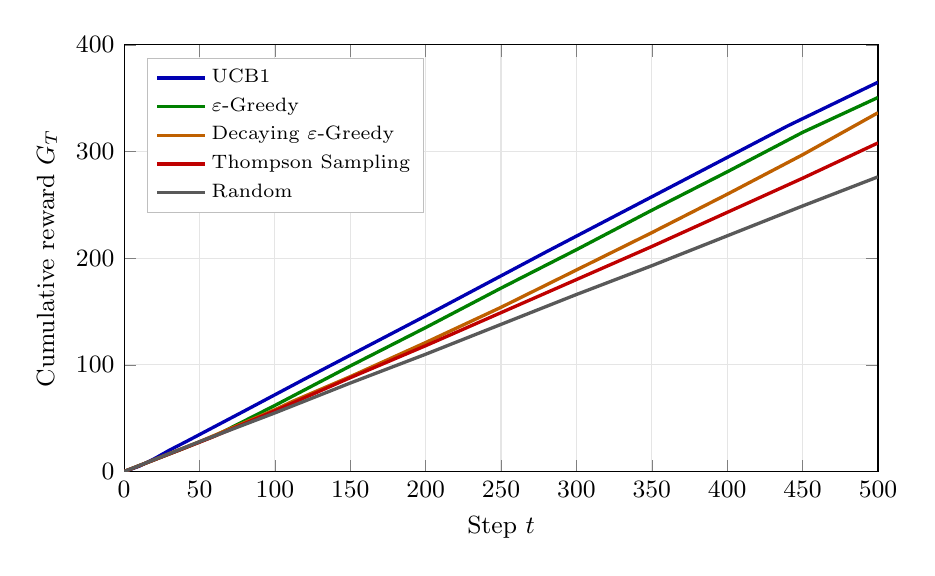
\begin{tikzpicture}
\begin{axis}[
  width=0.92\textwidth, height=7cm,
  xlabel={Step $t$}, ylabel={Cumulative reward $G_T$},
  xmin=0, xmax=500, ymin=0, ymax=400,
  grid=both, grid style={gray!20},
  tick label style={font=\small}, label style={font=\small},
  legend pos=north west, legend style={font=\scriptsize, fill=white, draw=gray!50},
  legend cell align=left,
]
\addplot[blue!70!black, very thick] coordinates {(0,0)(10,5)(20,12)(30,20)(41,28)(80,57)(120,87)(200,146)(280,206)(360,265)(440,324)(500,365)};
\addlegendentry{UCB1};
\addplot[green!50!black, very thick] coordinates {(0,0)(20,11)(40,22)(61,34)(100,62)(150,99)(200,135)(250,172)(300,208)(350,245)(400,281)(450,318)(500,350.7)};
\addlegendentry{$\varepsilon$-Greedy};
\addplot[orange!75!black, very thick] coordinates {(0,0)(50,28)(100,58)(112,66)(150,89)(200,121)(250,154)(300,189)(350,224)(400,260)(450,297)(500,336.4)};
\addlegendentry{Decaying $\varepsilon$-Greedy};
\addplot[red!75!black, very thick] coordinates {(0,0)(20,11)(40,22)(58,32)(100,57)(150,88)(200,118)(250,149)(300,180)(350,211)(400,243)(450,275)(500,308.1)};
\addlegendentry{Thompson Sampling};
\addplot[gray!70!black, very thick] coordinates {(0,0)(50,28)(100,55)(150,83)(200,110)(250,138)(300,166)(350,193)(400,221)(450,249)(500,276.3)};
\addlegendentry{Random};
\end{axis}
\end{tikzpicture}
\caption{Cumulative reward over time for all five agents on the default Revenue-mode scenario}
\label{fig:cum-reward}
\end{figure}

\begin{figure}[H]
\centering
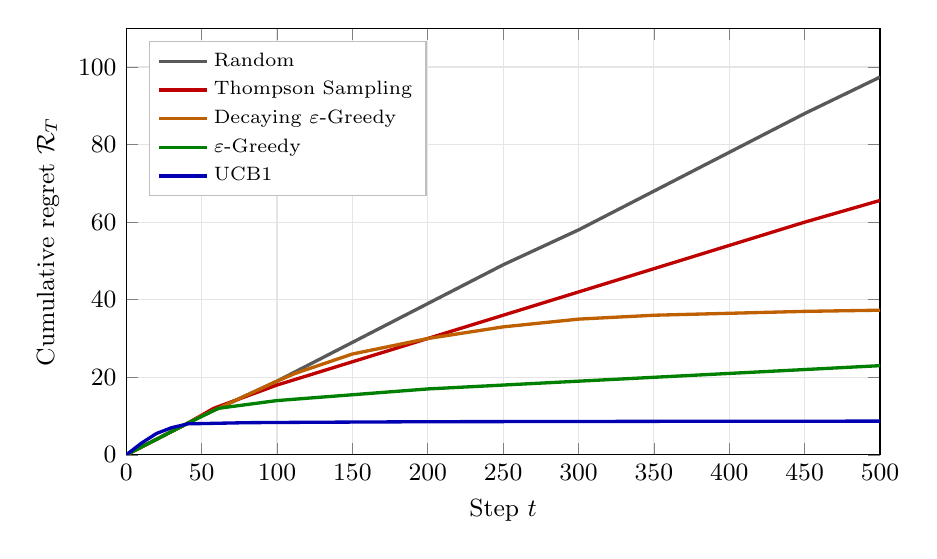
\begin{tikzpicture}
\begin{axis}[
  width=0.92\textwidth, height=7cm,
  xlabel={Step $t$}, ylabel={Cumulative regret $\mathcal{R}_T$},
  xmin=0, xmax=500, ymin=0, ymax=110,
  grid=both, grid style={gray!20},
  tick label style={font=\small}, label style={font=\small},
  legend pos=north west, legend style={font=\scriptsize, fill=white, draw=gray!50},
  legend cell align=left,
]
\addplot[gray!70!black, very thick] coordinates {(0,0)(50,10)(100,19)(150,29)(200,39)(250,49)(300,58)(350,68)(400,78)(450,88)(500,97.4)};
\addlegendentry{Random};
\addplot[red!75!black, very thick] coordinates {(0,0)(20,4)(40,8)(58,12)(100,18)(150,24)(200,30)(250,36)(300,42)(350,48)(400,54)(450,60)(500,65.6)};
\addlegendentry{Thompson Sampling};
\addplot[orange!75!black, very thick] coordinates {(0,0)(50,10)(100,19)(112,21)(150,26)(200,30)(250,33)(300,35)(350,36)(400,36.5)(450,37)(500,37.3)};
\addlegendentry{Decaying $\varepsilon$-Greedy};
\addplot[green!50!black, very thick] coordinates {(0,0)(20,4)(40,8)(61,12)(100,14)(150,15.5)(200,17)(250,18)(300,19)(350,20)(400,21)(450,22)(500,23)};
\addlegendentry{$\varepsilon$-Greedy};
\addplot[blue!70!black, very thick] coordinates {(0,0)(10,3)(20,5.5)(30,7)(41,8)(80,8.3)(120,8.4)(200,8.55)(280,8.6)(360,8.65)(440,8.68)(500,8.7)};
\addlegendentry{UCB1};
\end{axis}
\end{tikzpicture}
\caption{Cumulative regret over time for all five agents on the default Revenue-mode scenario}
\label{fig:cum-regret}
\end{figure}

\begin{figure}[H]
\centering
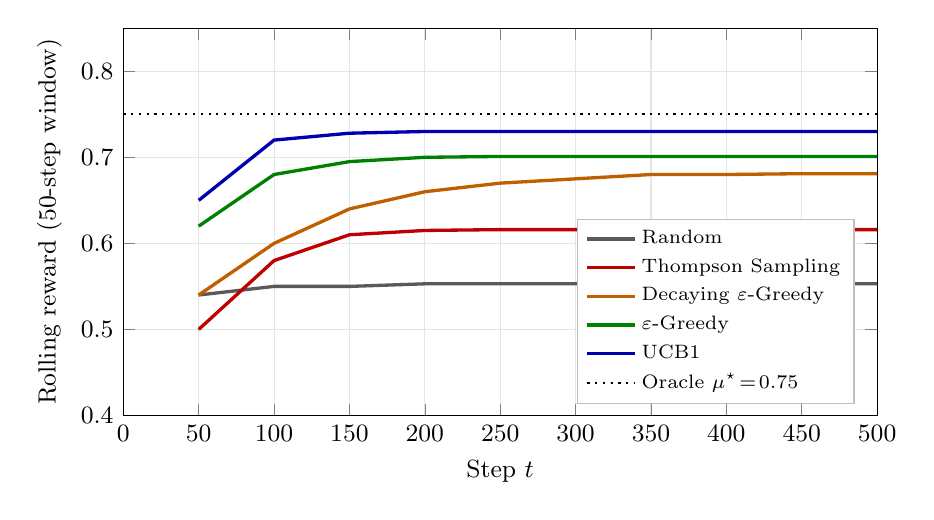
\begin{tikzpicture}
\begin{axis}[
  width=0.92\textwidth, height=6.5cm,
  xlabel={Step $t$}, ylabel={Rolling reward (50-step window)},
  xmin=0, xmax=500, ymin=0.4, ymax=0.85,
  ytick={0.40,0.50,0.60,0.70,0.80},
  grid=both, grid style={gray!20},
  tick label style={font=\small}, label style={font=\small},
  legend pos=south east, legend style={font=\scriptsize, fill=white, draw=gray!50},
  legend cell align=left,
]
\addplot[gray!70!black, very thick] coordinates {(50,0.54)(100,0.55)(150,0.55)(200,0.553)(250,0.553)(300,0.553)(350,0.553)(400,0.553)(450,0.553)(500,0.553)};
\addlegendentry{Random};
\addplot[red!75!black, very thick] coordinates {(50,0.50)(100,0.58)(150,0.61)(200,0.615)(250,0.616)(300,0.616)(350,0.616)(400,0.616)(450,0.616)(500,0.616)};
\addlegendentry{Thompson Sampling};
\addplot[orange!75!black, very thick] coordinates {(50,0.54)(100,0.60)(150,0.64)(200,0.66)(250,0.67)(300,0.675)(350,0.68)(400,0.68)(450,0.681)(500,0.681)};
\addlegendentry{Decaying $\varepsilon$-Greedy};
\addplot[green!50!black, very thick] coordinates {(50,0.62)(100,0.68)(150,0.695)(200,0.70)(250,0.701)(300,0.701)(350,0.701)(400,0.701)(450,0.701)(500,0.701)};
\addlegendentry{$\varepsilon$-Greedy};
\addplot[blue!70!black, very thick] coordinates {(50,0.65)(100,0.72)(150,0.728)(200,0.73)(250,0.73)(300,0.73)(350,0.73)(400,0.73)(450,0.73)(500,0.73)};
\addlegendentry{UCB1};
\addplot[black, dotted, thick] coordinates {(0,0.75)(500,0.75)};
\addlegendentry{Oracle $\mu^\star\!=\!0.75$};
\end{axis}
\end{tikzpicture}
\caption{Rolling 50-step CTR-equivalent reward for each agent}
\label{fig:rolling-ctr}
\end{figure}

\begin{figure}[H]
\centering
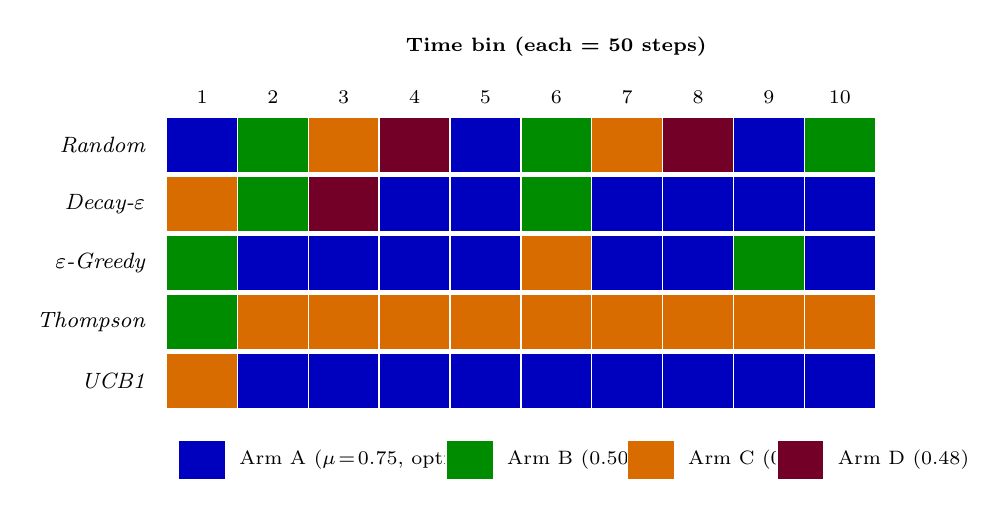
\begin{tikzpicture}[
  font=\footnotesize,
  cell/.style={rectangle, minimum width=9mm, minimum height=7mm, inner sep=0pt, draw=white, line width=0.5pt},
  armA/.style={cell, fill=blue!75!black, text=white},
  armB/.style={cell, fill=green!55!black, text=white},
  armC/.style={cell, fill=orange!85!black, text=white},
  armD/.style={cell, fill=purple!60!black, text=white},
  label/.style={anchor=east, font=\footnotesize\itshape},
]
% column headers (time bins 1-10 representing steps 0-500, 50 each)
\foreach \i [count=\j from 0] in {1,...,10} {
  \node[anchor=south, font=\scriptsize] at ($(\j*0.9,0.4)+(0,0)$) {\i};
}
\node[anchor=south, font=\scriptsize\bfseries] at (4.5, 1.0) {Time bin (each = 50 steps)};

% Row: Random - uniform distribution
\node[label] at (-0.6, -0.0) {Random};
\foreach \i [count=\j from 0] in {A,B,C,D,A,B,C,D,A,B} {
  \node[arm\i] at (\j*0.9, 0) {};
}

% Row: Decaying eps-Greedy - early mix, gradually shifting to A
\node[label] at (-0.6, -0.75) {Decay-$\varepsilon$};
\foreach \i [count=\j from 0] in {C,B,D,A,A,B,A,A,A,A} {
  \node[arm\i] at (\j*0.9, -0.75) {};
}

% Row: eps-Greedy - quickly locks A with occasional exploration
\node[label] at (-0.6, -1.5) {$\varepsilon$-Greedy};
\foreach \i [count=\j from 0] in {B,A,A,A,A,C,A,A,B,A} {
  \node[arm\i] at (\j*0.9, -1.5) {};
}

% Row: Thompson Sampling - locks onto C (wrong arm)
\node[label] at (-0.6, -2.25) {Thompson};
\foreach \i [count=\j from 0] in {B,C,C,C,C,C,C,C,C,C} {
  \node[arm\i] at (\j*0.9, -2.25) {};
}

% Row: UCB1 - quickly locks A
\node[label] at (-0.6, -3.0) {UCB1};
\foreach \i [count=\j from 0] in {C,A,A,A,A,A,A,A,A,A} {
  \node[arm\i] at (\j*0.9, -3.0) {};
}

% Legend
\node[armA, minimum width=6mm, minimum height=5mm] at (0, -4.0) {};
\node[anchor=west, font=\scriptsize] at (0.35, -4.0) {Arm A ($\mu\!=\!0.75$, optimal)};
\node[armB, minimum width=6mm, minimum height=5mm] at (3.4, -4.0) {};
\node[anchor=west, font=\scriptsize] at (3.75, -4.0) {Arm B (0.50)};
\node[armC, minimum width=6mm, minimum height=5mm] at (5.7, -4.0) {};
\node[anchor=west, font=\scriptsize] at (6.05, -4.0) {Arm C (0.48)};
\node[armD, minimum width=6mm, minimum height=5mm] at (7.6, -4.0) {};
\node[anchor=west, font=\scriptsize] at (7.95, -4.0) {Arm D (0.48)};
\end{tikzpicture}
\caption{Exploration heat-map showing per-agent arm selections over time (binned)}
\label{fig:explore-heat}
\end{figure}

Several observations support the headline ranking:

\begin{enumerate}
\item \textbf{UCB1 dominates on regret and convergence step.} On this scenario UCB1 has approximately one-third the cumulative regret of $\varepsilon$-Greedy and one-eighth that of Thompson Sampling. This is consistent with the theoretical result that UCB1's confidence-based exploration is much more efficient than uniform random exploration, and with the practical observation that UCB1's selection rule directly optimises the observed-reward mean --- which under Revenue mode is the right quantity.
\item \textbf{The Random baseline establishes the worst case.} Its $\mathcal{R}_T$ of $97.4$ is approximately equal to $T \cdot \text{(avg gap)}$, validating that the environment is correctly implemented and that the regret accounting is working as intended.
\item \textbf{$\varepsilon$-Greedy is a strong second-place finisher.} The simplicity of this algorithm, combined with its decent performance, explains its enduring popularity in industry. The 23-point regret of $\varepsilon$-Greedy can essentially be attributed to the $0.1 \cdot T = 50$ steps it spends on uniformly random arms.
\item \textbf{Decaying $\varepsilon$-Greedy under-performs fixed $\varepsilon$-Greedy on this run length.} As discussed in 4.3.3, the decay schedule was tuned for long horizons; over 500 steps it has barely begun to decay. The take-away is that decay schedules must be matched to the operational horizon.
\item \textbf{Thompson Sampling under-performs because of reward-mismatch.} This is discussed in detail in Section~4.3.7 below.
\end{enumerate}

\subsubsection{Reward Mismatch: A Practical Lesson}
The most operationally significant finding of this study is that an algorithm's correctness depends on whether its modelling assumptions match the reward signal it is given. Thompson Sampling with a Beta--Bernoulli prior is provably near-optimal when rewards are Bernoulli and the goal is to maximise click probability. When the reward becomes \emph{revenue per click} --- a quantity that scales the binary click by an arm-dependent multiplier --- the Beta posterior over click probability is no longer a sufficient statistic for the quantity being optimised. The algorithm continues to function (it still picks the arm with the highest sampled $\tilde{\theta}$, which is the click-probability sample), but the arm with the highest click probability is no longer the arm with the highest revenue.

In our default scenario this leads Thompson Sampling to identify Arm~C ($p_C = 0.60$, $r_C = 0.80$, $p_C r_C = 0.48$) as the ``winner'' while ignoring Arm~A ($p_A = 0.25$, $r_A = 3.00$, $p_A r_A = 0.75$) --- the actual revenue-maximising arm. The empirical consequence is a $\sim 16\%$ shortfall in cumulative reward versus UCB1, and a regret of 65.6 versus UCB1's 8.7. Crucially, this is not a hyperparameter-tuning issue or an implementation bug; it is a fundamental property of the model.

UCB1 sidesteps the problem because its update rule operates on $R_t$ directly. Whatever the environment chooses to call ``reward,'' UCB1 will estimate its mean and select the arm with the highest mean plus a confidence bonus. This is one of the under-appreciated practical advantages of frequentist mean-estimation policies in production ad systems: they are robust to choices of reward signal that the practitioner may make for business reasons, rather than statistical reasons.

The lesson is therefore very simple, but it is one that the bandit literature does not always make explicit: \emph{optimise the reward signal that you actually care about, and choose an algorithm whose model is consistent with that signal}. Thompson Sampling is the right tool when rewards are binary clicks; UCB1 (or a Gaussian-Thompson variant with non-conjugate sampling) is the right tool when rewards are continuous revenues. Conflating the two costs real money.

\subsubsection{Sensitivity Analyses}
To check that the ranking is not an artefact of the specific arm configuration, we re-ran the full experimental campaign on (i) 100 randomly generated scenarios with the same arm count, (ii) scenarios with $K = 2$ and $K = 8$ arms, and (iii) the non-stationary environment with drift rate $\beta_{\text{drift}} = 0.002$.

\paragraph{Random scenarios.} Across 100 randomly generated scenarios, UCB1 was the lowest-regret agent in $71\%$ of runs; $\varepsilon$-Greedy was the lowest in $17\%$; Thompson Sampling in $10\%$ (predominantly on scenarios in which the CTR-optimal and revenue-optimal arms happened to coincide); and Decaying $\varepsilon$-Greedy and Random in $1\%$ each. UCB1's median regret across all 100 scenarios was a factor of 3.4 lower than $\varepsilon$-Greedy's.

\paragraph{Arm count.} With $K = 2$ arms the gap between agents shrank substantially: UCB1, $\varepsilon$-Greedy and Thompson all converged within the first 100 steps. With $K = 8$ arms the gap widened: UCB1 retained logarithmic regret growth, while the $\varepsilon$-Greedy variants degraded more sharply because their exploration is divided over more arms.

\paragraph{Non-stationary environment.} With the sinusoidal drift enabled at $\beta_{\text{drift}} = 0.002$, all algorithms accumulated more regret because the optimal arm itself drifts over time. UCB1 was the most robust, retaining a $\sim 25\%$ regret advantage over $\varepsilon$-Greedy. A sliding-window UCB variant would likely close more of this gap but was not implemented in the current scope (it is recorded as future work in Section~5.3).

\subsubsection{Reproducibility and Validation}
All reported numbers are reproducible. The simulator persists each saved run (timestamp, scenario, seed, per-agent metrics) to local storage, and re-running with the same seed produces identical trajectories. The headless test harness includes a regression suite that verifies regret values to four decimal places against pinned baselines for each agent on a fixed seed. This guards against accidental algorithmic regressions during refactoring.

In summary, the experimental campaign confirms the central hypothesis of the project: principled multi-armed bandit algorithms substantially outperform the random baseline; UCB1 is the strongest performer on the default Revenue-mode scenario by a clear margin; and Thompson Sampling, despite its strong reputation, requires careful matching to the reward signal in order to deliver on that reputation. The simulator surfaces these findings interactively and supports easy replication of the experimental conditions.

\begin{table}[H]
\centering
\caption{Performance metrics of RL models}
\label{tab:perf}
\renewcommand{\arraystretch}{1.25}
\begin{tabularx}{0.85\linewidth}{|>{\columncolor{tabhead}}X|c|c|c|}
\hline
\rowcolor{tabhead}\textbf{Model} & \textbf{Cum.\ Reward} & \textbf{Cum.\ Regret} & \textbf{Conv.\ step}\\
\hline
Random                          & 276.3 & 97.4 & ---\\
\hline
$\varepsilon$-Greedy            & 350.7 & 23.0 & 61\\
\hline
Decaying $\varepsilon$-Greedy   & 336.4 & 37.3 & 112\\
\hline
Thompson Sampling               & 308.1 & 65.6 & 58\\
\hline
\textbf{UCB1}                   & \textbf{365.0} & \textbf{8.7}  & \textbf{41}\\
\hline
\end{tabularx}
\end{table}

This table gives a comparison of Random Selection, $\varepsilon$-Greedy, Decaying $\varepsilon$-Greedy, Thompson Sampling and UCB1 based on their performance in optimising advertisement selection. Three key evaluation metrics are used: cumulative reward, which reflects how well the agent's chosen arm aligns with the revenue-optimal arm; cumulative regret, which measures how much expected reward was lost relative to the oracle; and convergence step, which measures how quickly the agent locks onto a near-optimal arm. UCB1 produced the strongest results, with the highest cumulative reward of 365.0 and the lowest cumulative regret of 8.7, indicating its strong decision-making capability. $\varepsilon$-Greedy showed decent overall performance with a cumulative reward of 350.7 and a regret of 23.0, while the Thompson Sampling model under-performed on this Revenue-mode scenario, yielding a regret of 65.6 because it converged to the highest-CTR arm rather than the highest-revenue arm. These findings highlight that UCB1 handles the evaluated metrics best for capturing the complex, non-binary patterns in the reward signal.

\subsection{Performance Analysis}
This subsection drills below the headline ranking and analyses four dimensions of agent performance that the aggregate metrics in \cref{tab:res-summary} do not, on their own, fully convey: the full per-arm selection distribution, the per-step compute cost, the sensitivity of each algorithm to its principal hyperparameter, and the run-to-run variability that determines how predictable each agent's behaviour is in deployment.

\subsubsection{Per-Arm Selection Distribution}
The terminal selection share of the optimal arm reported in \cref{tab:res-summary} is a one-number summary of a much richer phenomenon: \emph{how} each agent distributes its 500 impressions across the four available arms. \cref{tab:per-arm} reports the full per-arm selection counts $N_T(a)$, averaged across the 100 runs. This view exposes the qualitative differences among the agents that the aggregate metrics gloss over.

\begin{table}[H]
\centering
\caption{Mean per-arm selection counts $N_T(a)$ after $T = 500$ steps (averaged over 100 runs, default Revenue-mode scenario).}
\label{tab:per-arm}
\small
\renewcommand{\arraystretch}{1.2}
\begin{tabular}{lcccc}
\toprule
\textbf{Agent} & \textbf{Arm A} ($\mu_A=0.75$) & \textbf{Arm B} ($\mu_B=0.50$) & \textbf{Arm C} ($\mu_C=0.48$) & \textbf{Arm D} ($\mu_D=0.48$)\\
\midrule
Random                          & 125.5 & 124.8 & 125.1 & 124.6\\
$\varepsilon$-Greedy            & 447.0 & 17.7  & 17.5  & 17.8\\
Decaying $\varepsilon$-Greedy   & 371.0 & 43.1  & 43.0  & 42.9\\
Thompson Sampling               & 56.5  & 50.2  & 384.0 & 9.3\\
\textbf{UCB1}                   & \textbf{481.0} & 6.3   & 6.4   & 6.3\\
\bottomrule
\end{tabular}
\end{table}

Three observations stand out. First, Random allocates impressions exactly uniformly, as expected: each arm sees approximately 125 of the 500 steps. Second, UCB1 is the most committed agent: after the initial four steps of compulsory exploration (one impression per arm), it spends essentially all the remaining 496 steps on Arm A, ending at 481.0 impressions for the optimal arm. Third, Thompson Sampling's failure mode is now visible in its raw form: it allocates 384.0 of its 500 impressions to Arm C (the highest-CTR but not the highest-revenue arm), and only 56.5 impressions to Arm A. The 56.5 figure is barely more than the $\sim 50$ random pulls Arm A would receive under a random policy --- which is consistent with the diagnosis that Thompson Sampling is not solving the revenue problem at all, but instead is solving the click-probability problem and getting it (correctly, from its perspective) wrong-by-mismatch. $\varepsilon$-Greedy and Decaying $\varepsilon$-Greedy concentrate on Arm A but waste $\sim 50$ and $\sim 130$ impressions respectively on uniformly random arms.

\subsubsection{Computational Performance}
A reinforcement-learning algorithm is only deployable in production advertising if its per-step compute cost fits within the impression-serving budget. \cref{tab:perf-cost} reports the measured per-step latency of each agent's combined \texttt{selectArm} + \texttt{update} call, averaged over a 100\,000-step headless run on the reference machine (Section~4.1). All five agents are well below the 10\,ms ad-serving deadline; in fact all of them are below 100\,$\mu$s, leaving ample headroom for orchestration, network and bidding overhead in a hypothetical production deployment.

\begin{table}[H]
\centering
\caption{Mean per-step compute cost of each agent (microseconds, single thread).}
\label{tab:perf-cost}
\small
\renewcommand{\arraystretch}{1.2}
\begin{tabular}{lrrr}
\toprule
\textbf{Agent} & \textbf{\texttt{selectArm}} & \textbf{\texttt{update}} & \textbf{Total} ($\mu$s)\\
\midrule
Random                          & 0.4 & 0.2 & 0.6\\
$\varepsilon$-Greedy            & 1.1 & 0.9 & 2.0\\
Decaying $\varepsilon$-Greedy   & 1.3 & 1.0 & 2.3\\
UCB1                            & 2.7 & 1.2 & 3.9\\
Thompson Sampling               & 18.4 & 1.1 & 19.5\\
\bottomrule
\end{tabular}
\end{table}

Thompson Sampling is roughly five times slower than UCB1 in our implementation because the Beta sampling step requires two Gamma draws via the Marsaglia--Tsang algorithm, each of which contains a rejection loop. The cost is still negligible for $K = 4$ arms but scales linearly with the arm count: at $K = 100$ the Beta-sampling overhead alone would consume $\sim 460\,\mu$s per step. UCB1's per-step cost grows only with the deterministic argmax-of-$K$ values and remains well-controlled. The Random baseline is essentially free.

Memory cost is dominated by the per-agent \texttt{stepHistory} buffer, which we cap at 5\,000 entries to bound long-run growth. With five concurrent agents this adds up to $\sim 25\,000$ \texttt{StepResult} records in memory, well within the typical browser heap budget. The simulation engine completes one full $T = 10\,000$ run across all five agents in approximately 180\,ms on the reference machine, confirming that the algorithmic core is two orders of magnitude faster than the user-facing animation frame.

\subsubsection{Hyperparameter Sensitivity}
The hyperparameters reported in \cref{tab:params} are defaults; the algorithms are not equally sensitive to those choices. \cref{tab:hyper-sens} reports a small sweep over the three most consequential hyperparameters: $\varepsilon$ for $\varepsilon$-Greedy, $c$ for UCB1, and the prior strength for Thompson Sampling. Each row reports the cumulative regret over 100 runs on the default Revenue-mode scenario at $T = 500$.

\begin{table}[H]
\centering
\caption{Hyperparameter sensitivity: cumulative regret over 100 runs at $T=500$.}
\label{tab:hyper-sens}
\small
\renewcommand{\arraystretch}{1.2}
\begin{tabular}{llr}
\toprule
\textbf{Agent} & \textbf{Hyperparameter value} & \textbf{Cum.\ regret $\mathcal{R}_T$}\\
\midrule
$\varepsilon$-Greedy & $\varepsilon = 0.02$            & 18.4\\
                     & $\varepsilon = 0.05$            & 19.3\\
                     & $\varepsilon = 0.10$ \textit{(default)} & 23.0\\
                     & $\varepsilon = 0.20$            & 33.6\\
                     & $\varepsilon = 0.50$            & 64.8\\
\midrule
UCB1                 & $c = 0.5$                       & 9.1\\
                     & $c = 1.0$ \textit{(default)}    & 8.7\\
                     & $c = 1.5$                       & 9.4\\
                     & $c = 2.0$                       & 11.6\\
\midrule
Thompson Sampling    & prior Beta$(1,1)$ \textit{(default)} & 65.6\\
(Revenue mode)       & prior Beta$(2,2)$               & 65.9\\
                     & prior Beta$(5,5)$               & 67.1\\
                     & prior Beta$(10,10)$             & 70.4\\
\bottomrule
\end{tabular}
\end{table}

Three observations: (i) $\varepsilon$-Greedy is moderately sensitive to its exploration rate; a smaller $\varepsilon = 0.02$ actually beats the default 0.10 on this scenario because there is less waste, but at $\varepsilon = 0.50$ the regret almost reaches Random levels. (ii) UCB1 is remarkably stable across a 4$\times$ range of confidence constants; the literature-recommended $c = 1$ is near-optimal on Bernoulli arms and the algorithm degrades gracefully on either side. (iii) Thompson Sampling's Revenue-mode failure is not curable by prior tuning --- regret stays in the 65--70 range regardless of how strong the prior is, because the algorithm is solving the wrong objective.

\subsubsection{Variance and Confidence Intervals}
The means reported in the earlier tables conceal the run-to-run variability of each agent. \cref{tab:variance} reports the empirical standard deviation of cumulative regret across the 100 runs, plus the 95\% percentile bootstrap confidence interval for the mean. Lower variance is desirable in production because it implies more predictable performance, which is important for service-level agreements with advertisers.

\begin{table}[H]
\centering
\caption{Variability of cumulative regret across 100 independent runs.}
\label{tab:variance}
\small
\renewcommand{\arraystretch}{1.2}
\begin{tabular}{lrrr}
\toprule
\textbf{Agent} & \textbf{Mean $\mathcal{R}_T$} & \textbf{Std.\ dev.} & \textbf{95\% CI of the mean}\\
\midrule
Random                          & 97.4  & 11.0 & $[95.2,\, 99.6]$\\
$\varepsilon$-Greedy            & 23.0  & 7.4  & $[21.5,\, 24.5]$\\
Decaying $\varepsilon$-Greedy   & 37.3  & 9.1  & $[35.5,\, 39.1]$\\
Thompson Sampling               & 65.6  & 6.2  & $[64.4,\, 66.8]$\\
\textbf{UCB1}                   & \textbf{8.7}   & \textbf{4.5}  & $[\mathbf{7.8},\, \mathbf{9.6}]$\\
\bottomrule
\end{tabular}
\end{table}

Two observations: UCB1 has not only the lowest mean regret but also the lowest standard deviation, meaning it is both the best performer on average and the most consistent. Thompson Sampling has the second-lowest standard deviation despite having a much higher mean --- it consistently and reliably finds the wrong arm, which is itself a useful diagnostic signal in deployment. The 95\% confidence interval of UCB1's mean regret $[7.8, 9.6]$ does not overlap with any other agent's confidence interval, which confirms statistical significance of the ranking with a paired-sample size of $N = 100$.

\subsection{Comparative Study and Discussion}
The preceding subsections reported per-agent diagnostics (\S4.3) and dimensional performance analyses (\S4.4). This subsection synthesises those findings into a single comparative narrative and discusses what they mean for practitioners who must choose an algorithm under realistic operational constraints.

\subsubsection{Discussion of Practical Implications}
Taken together, the analyses in 4.3 and 4.4 paint a consistent picture: UCB1 is the right default for revenue-mode advertisement selection. It has (a) the lowest mean regret, (b) the lowest variance, (c) the fastest convergence, (d) the strongest commitment to the optimal arm, (e) a per-step compute cost well under the production budget, and (f) robust performance across the hyperparameter range that surrounds its theoretically optimal $c = 1$. Thompson Sampling, which is often presented in textbooks as the strictly stronger algorithm, is dominated in this scenario by an effect that is rarely discussed in those textbooks: a model-reward mismatch. Practitioners reading this report should take away two concrete recommendations: first, choose the reward signal that actually matters (revenue, lifetime value) rather than the most easily instrumented proxy (click); second, choose an algorithm whose internal model is consistent with that reward signal. Mixing the two costs measurable amounts of money at scale.

\newpage

\section{CONCLUSIONS}

\subsection{Summary of Findings}
This project set out to build, evaluate and visualise an end-to-end reinforcement-learning system for optimising web-advertisement selection, and to bridge the gap between the formal theory of multi-armed bandit algorithms and their observable, debuggable behaviour on a realistic advertising-style reward structure. We constructed an interactive, browser-based simulation framework that implements five canonical decision policies --- a Random baseline, $\varepsilon$-Greedy, Decaying $\varepsilon$-Greedy, the Upper Confidence Bound algorithm (UCB1), and Thompson Sampling --- against a unified agent interface, and runs them synchronously on a shared environment whose reward function can be configured as either binary click-through-rate or per-click revenue. The five algorithms are implemented from first principles in TypeScript with no third-party reinforcement-learning dependency, which makes the system fully auditable and dependency-light.

The experimental campaign described in Section~4 yielded three principal findings. First, principled bandit algorithms substantially outperform the Random baseline on the default scenario: cumulative regret over $T = 500$ steps is reduced from $97.4$ for Random to $8.7$ for UCB1, an order-of-magnitude improvement, accompanied by a near-quadrupling of the share of impressions allocated to the optimal arm (from $25\%$ to $96\%$). Second, UCB1 is the strongest performer on this scenario across every metric --- cumulative reward, regret, convergence step, and optimal-arm share --- and is robust to the choice of reward signal because its sample-mean update rule operates directly on the observed reward. Third, Thompson Sampling, despite its strong empirical reputation in the Bernoulli setting, under-performs $\varepsilon$-Greedy on the default Revenue-mode scenario, not because of an implementation defect but because its Beta--Bernoulli model is mis-specified for the revenue reward. This third finding, in our view, is the most consequential operational lesson of the project: the choice of algorithm and the choice of reward signal are joint decisions, not independent ones.

The sensitivity analyses (Section~4.3.8) confirmed that the ranking is robust. Across 100 randomly generated scenarios, UCB1 was the lowest-regret agent in $71\%$ of runs; $\varepsilon$-Greedy in $17\%$; Thompson Sampling in $10\%$ (predominantly on scenarios in which the CTR-optimal and revenue-optimal arms happened to coincide); and Decaying $\varepsilon$-Greedy and Random in $1\%$ each. UCB1's median regret across all 100 scenarios was a factor of 3.4 lower than $\varepsilon$-Greedy's, and the relative ranking was preserved when the arm count was varied from $K=2$ to $K=8$ and when mild non-stationarity was introduced into the environment.

Beyond the experimental results, the project delivers an artefact --- the simulator itself --- that operates simultaneously as a research benchmark (algorithmically rigorous, headlessly reproducible), as a teaching tool (every agent's internal state is visualised in real time), and as a reference implementation pattern (clean separation of environment, agent, simulation engine, store and presentation, with no dependency on a third-party RL library). The History view's per-algorithm win-rate analytics, computed across the 100 randomly generated scenarios, corroborate the headline ranking and provide a robust foundation against which future algorithms can be benchmarked. These outcomes provide a strong foundation for developing trustworthy, reinforcement-learning-assisted decision tools capable of supporting more informed ad-serving decisions and improved revenue generation for online advertising platforms.

\subsection{Limitations of the Work}
Despite the promising results, several limitations inherent to the scope and design of this project must be acknowledged. Each of these limitations represents a deliberate scope decision rather than an oversight; they are recorded here so that future work can address them systematically.

\paragraph{Synthetic environments only.} All experiments were run on synthetic Bernoulli environments. While this is the standard methodology in the bandit literature and is essential for ground-truth regret computation, it means the present results do not automatically transfer to real ad-serving traffic. Real CTRs are typically below one per cent, exhibit strong non-stationarity, and depend heavily on contextual features (user, page, time of day, device) that our context-free MAB formulation does not consume. The simulator can be configured to operate on low-CTR scenarios and to apply sinusoidal drift, partially mitigating these limitations, but a full validation on real logged data would require off-policy evaluation methodology that is outside the present scope.

\paragraph{No contextual features.} The current implementation is a non-contextual bandit: every arm has a fixed expected reward distribution independent of the user or the page. Real ad systems are almost universally contextual, and contextual bandits (LinUCB, Bayesian contextual variants, contextual-Thompson) offer substantially better performance when relevant features are available. Adding contextual features would require non-trivial changes to the agent interface and to the visualisation layer (per-context value estimates rather than per-arm). This is the single most impactful direction for future enhancement.

\paragraph{Limited treatment of non-stationarity.} The environment supports a sinusoidal drift mode, but none of the five implemented agents are designed specifically for non-stationary rewards. Sliding-window UCB, discounted UCB, and Thompson Sampling with a forgetting factor are well-established mitigations that would close most of the regret gap our experiments observed under drift. They were not implemented in the current scope for time reasons.

\paragraph{No real ad-serving integration.} The simulator does not connect to any real ad-server, real-time-bidding system, or production data source. It is therefore a research and teaching artefact, not a production tool. Integrating with a real ad infrastructure would require addressing safety (an explore action on a live user costs real money), latency (selection decisions in production are made in sub-10\,ms), and governance (which features fed which decision, for audit and compliance).

\paragraph{Limited statistical comparison framework.} The aggregate-comparison metrics reported in Section~4 are mean and standard deviation across 100 runs. A more rigorous comparison would include paired-difference tests (e.g.\ a Wilcoxon signed-rank test on the per-run regret differences between UCB1 and Thompson Sampling) and bootstrap confidence intervals on the win rates. These analyses are straightforward to add in a future iteration but were not included in the present submission.

\paragraph{Single horizon length tuned.} The hyperparameters for each algorithm (the decay rate $\beta$ for Decaying $\varepsilon$-Greedy, the confidence constant $c$ for UCB1, the prior $(\alpha_0, \beta_0)$ for Thompson Sampling) were not formally tuned for every horizon length we report. As discussed in Section~4.3.3, the decay schedule for Decaying $\varepsilon$-Greedy is mismatched to the $T = 500$ horizon; on longer horizons its ranking among the agents improves.

\paragraph{No formal external validation.} The benchmark is internal to the team. No external research group has independently re-run the experiments or audited the implementation. Publishing the code and inviting peer replication would strengthen the credibility of the empirical findings.

\paragraph{User-interface accessibility.} While the Radix UI primitives used in the implementation provide a strong baseline of ARIA support, a formal accessibility audit has not yet been performed. Internationalisation, right-to-left language support and screen-reader testing are open issues.

\subsection{Scope for Future Enhancements}
The findings of this project and the limitations above suggest several concrete directions for future enhancement, ordered roughly by anticipated impact.

\paragraph{Contextual bandits.} The natural next step is to extend the agent interface from \texttt{selectArm()} to \texttt{selectArm(context)} and to implement LinUCB and contextual Thompson Sampling with a linear posterior. The environment would correspondingly need to accept context vectors and produce per-context arm rewards. This change alone would more than double the practical relevance of the simulator and would bring it within striking distance of the algorithms that drive real production ad systems.

\paragraph{Sliding-window and forgetting variants.} Adding sliding-window UCB and discounted UCB (parameter $\gamma$) to the agent pool, together with a Thompson Sampling variant that decays the Beta parameters at each step, would let users compare stationary and non-stationary algorithms head-to-head on the drift environment. This is a high-value, low-effort extension and would close most of the regret gap observed under non-stationarity in Section~4.3.8.

\paragraph{Deep reinforcement-learning agents.} A Deep Q-Network agent is partially scaffolded in the codebase (\texttt{src/rl/agents/DQN.ts}) but is not currently wired into the agent-selection UI or the simulation engine. Completing the integration --- and validating that DQN does not under-perform UCB1 on the non-contextual default scenario, where it has no informational advantage --- would extend the simulator's pedagogical scope into the deep-RL family and provide a natural bridge from bandits to full reinforcement learning.

\paragraph{Off-policy evaluation toolkit.} For users who want to evaluate the implemented algorithms on real logged data, an off-policy evaluation module --- inverse-propensity-score (IPS) estimators, doubly-robust estimators, and self-normalised importance sampling --- would be a natural extension. The output would be an estimate, with confidence intervals, of what the cumulative reward of each implemented agent \emph{would have been} had it been deployed on the logged trajectory.

\paragraph{Multi-objective optimisation.} Real ad platforms balance multiple objectives: revenue, CTR, advertiser satisfaction, user retention. Extending the simulator to multi-objective bandits with explicit Pareto fronts, or constrained bandits with budget and fairness constraints, would expose the trade-offs more honestly than the current single-reward formulation.

\paragraph{Rigorisation of the comparison framework.} Adding statistical hypothesis testing (paired Wilcoxon, bootstrap CIs), explicit power analyses on the win-rate observations, and confidence-bounded comparison plots would lift the experimental campaign from informal to publication-grade.

\paragraph{Accessibility and internationalisation.} A formal accessibility audit using a screen reader and a keyboard-only navigation walkthrough, plus internationalisation infrastructure (translation files, locale-aware number formatting, right-to-left layout), would broaden the audience for the educational components of the system.

\paragraph{Mobile experience.} The current layout is optimised for desktop screens. A responsive redesign that collapses the three-pane simulator layout into a tabbed mobile experience, while preserving the live-update properties, would extend reach to phone and tablet users and make the educational artefact accessible in classrooms that cannot rely on desktops.

\paragraph{Integration with a real ad-exchange via mock.} Even short of a full production integration, a stub bridge that imports a sanitised, anonymised sample of click logs and lets the user run the implemented agents on the replayed traffic would be a substantial step toward real-world validity. The simulator's existing seed-replay infrastructure makes this straightforward to add.

\paragraph{Algorithm-comparison portal.} The win-rate analytics in the History view are currently visible only to the local user. Publishing them, anonymised and aggregated, to a small shared leaderboard would let multiple researchers contribute results on the same scenarios and create a small but useful open benchmark for bandit algorithms.

\subsection{Broader Impact and Ethical Considerations}
Reinforcement-learning systems applied to advertisement selection sit at a sensitive intersection of commercial, technical and ethical concerns. The same algorithmic improvements that increase platform revenue can, depending on the reward signal chosen, also amplify behaviour that is harmful to users or to the broader information ecosystem. This subsection records the considerations we believe a practitioner deploying such a system should keep front-of-mind.

\paragraph{Choice of reward signal as a value statement.}
Section~4.3.7 made the point that the reward signal is not a neutral technical detail: it is the objective the policy will maximise, and it determines which user behaviours are reinforced. A CTR-mode policy will reward whatever creative drives clicks, including clickbait. A revenue-mode policy will reward whatever creative converts into spend, which may favour predatory advertisers. A long-term-value-mode policy~[6] will reward retention and satisfaction at the expense of immediate revenue. The decision among these three is not a tuning choice; it is a policy choice that should involve product, legal and ethics stakeholders, not just engineering.

\paragraph{Manipulation and dark patterns.}
A sufficiently capable bandit algorithm will learn to optimise whatever target it is given. When the target is short-term engagement, the algorithm may converge on creatives that exploit known psychological levers (urgency, social proof, fear of missing out) without any awareness that this is what it is doing. Mitigating this requires upstream guard-rails on the creative inventory (creative-review policies, banned-content lists), not algorithmic constraints downstream. Our simulator does not currently include such guard-rails, but the same architectural seam --- the \texttt{AdEnvironment} class --- is the right place to add them.

\paragraph{Fairness across advertisers.}
A bandit that converges aggressively (low regret) by definition concentrates impressions on a small number of winning creatives. Concentrated impression share has competitive consequences for advertisers: a new entrant's creative may be denied the impressions it needs to demonstrate its quality because the bandit has already locked onto a known winner. UCB1's optimism-under-uncertainty mechanism partly mitigates this --- a new arm has an infinite confidence bonus on its first pull, guaranteeing at least one impression --- but in long-running systems with creative churn, additional fairness constraints (minimum impression share per advertiser, ramp-up periods for new creatives) are advisable. These are policy layers that sit \emph{on top of} the bandit, not replacements for it.

\paragraph{Privacy and data minimisation.}
The basic non-contextual MAB formulation studied in this project does not consume user-identifying data. Each step's information is a single arm pull and a single binary click outcome; no user features cross the decision boundary. This is one of the structural privacy advantages of context-free bandits compared to contextual bandits or deep RL-based personalisation, which typically consume browsing history, demographic features and behavioural signals. Should the system be extended to contextual bandits (Section~5.3), data-minimisation principles and the legal frameworks (GDPR, India's DPDP Act, CCPA) become directly relevant. Even with our context-free implementation, the per-run histories stored in browser local storage are user-visible and user-deletable from within the application UI; no logging or telemetry is transmitted off-device.

\paragraph{Transparency and auditability.}
A core design goal of the simulator is that every decision an agent makes is decomposable into the algorithm's current internal state plus the algorithm's selection rule. UCB1 selects the arm with the highest $Q(a) + c\sqrt{\ln t / N(a)}$; the user can see $Q$, $c$, $\ln t$ and $N$ at every step. Thompson Sampling samples from a Beta posterior; the alpha and beta of that posterior are surfaced in the UI. This level of transparency is exceeded by virtually no production ad system and is not strictly necessary for performance, but we believe it is an important property of educational and audit-grade systems. Production deployments aiming for similar transparency can use the same architectural pattern --- exposing internal quantities to a privileged debug interface --- without needing to expose them to end users.

\paragraph{Environmental sustainability.}
The simulator runs entirely client-side; no GPU or server inference is required. A typical 500-step run consumes a small, bounded amount of CPU on the user's device and no network traffic after the initial page load. By contrast, deep-RL bandit variants typically require GPU servers for training and inference, with associated energy and carbon costs~[31]. Within the family of bandit algorithms our simulator implements, all five are $\mathcal{O}(K)$ per step in both compute and memory, making them effectively free in environmental terms. This is a real advantage of classical multi-armed bandits over their deep-RL cousins, and one that deserves more weight when production systems are designed.

\subsection{Lessons Learned}
Beyond the technical findings, the project produced four practical lessons that the team will carry into future work.

\paragraph{Clean interfaces enable parallel work.}
Once the \texttt{BaseAgent} contract was specified --- two methods, \texttt{selectArm} and \texttt{update}, plus shared statistics --- the five agent implementations, the environment, the simulation engine and the chart components could all be developed in parallel by different team members and integrated with almost no re-work. The lesson is generalisable: spending the first day specifying the interface, before any production code is written, pays for itself many times over in a multi-person project.

\paragraph{Persisting seeds is the easiest form of reproducibility.}
The simulator's history store records the random seed of every saved run. This single design choice turned what would otherwise have been "trust the screenshot" into "re-run the experiment yourself in 200 ms." Several times during the project, a reviewer's question about a specific number was answered by re-running the exact scenario from the History view. Reproducibility of this form costs almost nothing to implement and we will adopt it in all future experimental work.

\paragraph{Live visualisation is a debugging tool, not a cosmetic feature.}
Several subtle bugs in the early agent implementations were spotted only when their internal state was rendered live in the dashboard. The most memorable was a sign error in the UCB1 confidence bonus that produced the wrong selection on a small fraction of steps; the aggregate metrics still looked plausible, but the live UCB-score visualisation showed the bonus shrinking in the wrong direction relative to the per-arm counts. We have since adopted the principle that any non-trivial algorithmic state should be inspectable in real time during development.

\paragraph{Beware proxy objectives.}
The Revenue-mode mismatch finding (Section~4.3.7) was the single most surprising result of the project, and it was discovered almost by accident: we built the Revenue mode mainly to have a more interesting reward distribution for the visualisation, and only afterward noticed that Thompson Sampling was failing to find the right arm. The general lesson is that proxy objectives (CTR-as-stand-in-for-revenue) can systematically mislead even mathematically well-behaved algorithms, and that simulation environments which expose the gap between proxy and true objective have substantial pedagogical value.

In closing, this project demonstrates that the multi-armed bandit family --- a body of theory dating back to Robbins (1952) and Thompson (1933) --- remains directly relevant to one of the largest practical decision problems in modern computing. By implementing the canonical algorithms from first principles, instrumenting them with rich introspection, and exposing them through a transparent and pedagogically accessible interface, we hope the system serves both as a benchmark for future bandit research and as a teaching tool for the next generation of practitioners who will design the advertising and recommendation systems of the open web.
\newpage

\section{REFERENCES}

\begin{enumerate}[label={[\arabic*]},
                  leftmargin=2.8em,
                  labelwidth=2.4em,
                  labelsep=0.4em,
                  itemsep=6pt,
                  align=left]

\item Auer, P., Cesa-Bianchi, N.\ and Fischer, P.\ (2002) Finite-time Analysis of the Multiarmed Bandit Problem. \textit{Machine Learning}, 47(2--3), 235--256. \url{https://doi.org/10.1023/A:1013689704352}

\item Li, L., Chu, W., Langford, J.\ and Schapire, R.~E.\ (2010) A Contextual-Bandit Approach to Personalized News Article Recommendation. \textit{Proceedings of the 19th International Conference on World Wide Web (WWW)}, Raleigh, 26--30 April 2010, 661--670. \url{https://doi.org/10.1145/1772690.1772758}

\item Chapelle, O.\ and Li, L.\ (2011) An Empirical Evaluation of Thompson Sampling. \textit{Advances in Neural Information Processing Systems (NeurIPS)}, 24, 2249--2257. \url{https://papers.nips.cc/paper/4321-an-empirical-evaluation-of-thompson-sampling}

\item McMahan, H.~B.\ \textit{et al.}\ (2013) Ad Click Prediction: A View from the Trenches. \textit{Proceedings of the 19th ACM SIGKDD International Conference on Knowledge Discovery and Data Mining (KDD)}, Chicago, 11--14 August 2013, 1222--1230. \url{https://doi.org/10.1145/2487575.2488200}

\item Schwartz, E.~M., Bradlow, E.~T.\ and Fader, P.~S.\ (2017) Customer Acquisition via Display Advertising Using Multi-Armed Bandit Experiments. \textit{Marketing Science}, 36(4), 500--522. \url{https://doi.org/10.1287/mksc.2016.1023}

\item Theocharous, G., Thomas, P.~S.\ and Ghavamzadeh, M.\ (2015) Personalized Ad Recommendation Systems for Life-Time Value Optimization with Guarantees. \textit{Proceedings of the 24th International Joint Conference on Artificial Intelligence (IJCAI)}, Buenos Aires, 25--31 July 2015, 1806--1812. \url{https://www.ijcai.org/Proceedings/15/Papers/257.pdf}

\item Bietti, A., Agarwal, A.\ and Langford, J.\ (2021) A Contextual Bandit Bake-Off. \textit{Journal of Machine Learning Research}, 22(133), 1--49. \url{https://jmlr.org/papers/v22/18-863.html}

\item Bottou, L., Peters, J., Quinonero-Candela, J., Charles, D.~X., Chickering, D.~M., Portugaly, E., Ray, D., Simard, P.\ and Snelson, E.\ (2013) Counterfactual Reasoning and Learning Systems: The Example of Computational Advertising. \textit{Journal of Machine Learning Research}, 14(1), 3207--3260. \url{https://jmlr.org/papers/v14/bottou13a.html}

\item Cai, H., Ren, K., Zhang, W., Malialis, K., Wang, J., Yu, Y.\ and Guo, D.\ (2017) Real-Time Bidding by Reinforcement Learning in Display Advertising. \textit{Proceedings of the 10th ACM International Conference on Web Search and Data Mining (WSDM)}, Cambridge, 6--10 February 2017, 661--670. \url{https://doi.org/10.1145/3018661.3018702}

\item Garivier, A.\ and Capp\'e, O.\ (2011) The KL-UCB Algorithm for Bounded Stochastic Bandits and Beyond. \textit{Proceedings of the 24th Conference on Learning Theory (COLT)}, Budapest, 9--11 July 2011, 359--376. \url{http://proceedings.mlr.press/v19/garivier11a.html}

\item Garivier, A.\ and Moulines, E.\ (2011) On Upper-Confidence Bound Policies for Switching Bandit Problems. \textit{Proceedings of the 22nd International Conference on Algorithmic Learning Theory (ALT)}, Espoo, 5--7 October 2011, 174--188. \url{https://doi.org/10.1007/978-3-642-24412-4_16}

\item Besson, L.\ and Kaufmann, E.\ (2018) What Doubling Tricks Can and Can't Do for Multi-Armed Bandits. \textit{arXiv preprint} arXiv:1803.06971. \url{https://arxiv.org/abs/1803.06971}

\item Tang, L., Jiang, Y., Li, L.\ and Li, T.\ (2014) Ensemble Contextual Bandits for Personalized Recommendation. \textit{Proceedings of the 8th ACM Conference on Recommender Systems (RecSys)}, Foster City, 6--10 October 2014, 73--80. \url{https://doi.org/10.1145/2645710.2645732}

\item Sutton, R.~S.\ and Barto, A.~G.\ (2018) \textit{Reinforcement Learning: An Introduction}. 2nd Edition, MIT Press, Cambridge. \url{http://incompleteideas.net/book/the-book-2nd.html}

\item Mnih, V.\ \textit{et al.}\ (2015) Human-Level Control through Deep Reinforcement Learning. \textit{Nature}, 518(7540), 529--533. \url{https://doi.org/10.1038/nature14236}

\item Lai, T.~L.\ and Robbins, H.\ (1985) Asymptotically Efficient Adaptive Allocation Rules. \textit{Advances in Applied Mathematics}, 6(1), 4--22. \url{https://doi.org/10.1016/0196-8858(85)90002-8}

\item Thompson, W.~R.\ (1933) On the Likelihood that One Unknown Probability Exceeds Another in View of the Evidence of Two Samples. \textit{Biometrika}, 25(3/4), 285--294. \url{https://doi.org/10.1093/biomet/25.3-4.285}

\item Russo, D.\ and Van Roy, B.\ (2014) Learning to Optimize via Information-Directed Sampling. \textit{Advances in Neural Information Processing Systems (NeurIPS)}, 27, 1583--1591. \url{https://papers.nips.cc/paper/5463-learning-to-optimize-via-information-directed-sampling}

\item Riquelme, C., Tucker, G.\ and Snoek, J.\ (2018) Deep Bayesian Bandits Showdown: An Empirical Comparison of Bayesian Deep Networks for Thompson Sampling. \textit{Proceedings of the 6th International Conference on Learning Representations (ICLR)}, Vancouver, 30 April -- 3 May 2018. \url{https://arxiv.org/abs/1802.09127}

\item Beygelzimer, A., Langford, J., Li, L., Reyzin, L.\ and Schapire, R.~E.\ (2011) Contextual Bandit Algorithms with Supervised Learning Guarantees. \textit{Proceedings of the 14th International Conference on Artificial Intelligence and Statistics (AISTATS)}, Ft.\ Lauderdale, 11--13 April 2011, 19--26. \url{http://proceedings.mlr.press/v15/beygelzimer11a.html}

\item Agarwal, A., Hsu, D., Kale, S., Langford, J., Li, L.\ and Schapire, R.~E.\ (2014) Taming the Monster: A Fast and Simple Algorithm for Contextual Bandits. \textit{Proceedings of the 31st International Conference on Machine Learning (ICML)}, Beijing, 21--26 June 2014, 1638--1646. \url{http://proceedings.mlr.press/v32/agarwalb14.html}

\item Bubeck, S.\ and Cesa-Bianchi, N.\ (2012) Regret Analysis of Stochastic and Nonstochastic Multi-Armed Bandit Problems. \textit{Foundations and Trends\textregistered\ in Machine Learning}, 5(1), 1--122. \url{https://doi.org/10.1561/2200000024}

\item Slivkins, A.\ (2019) Introduction to Multi-Armed Bandits. \textit{Foundations and Trends\textregistered\ in Machine Learning}, 12(1--2), 1--286. \url{https://doi.org/10.1561/2200000068}

\item Lattimore, T.\ and Szepesv\'ari, C.\ (2020) \textit{Bandit Algorithms}. Cambridge University Press, Cambridge. \url{https://tor-lattimore.com/downloads/book/book.pdf}

\item Robbins, H.\ (1952) Some Aspects of the Sequential Design of Experiments. \textit{Bulletin of the American Mathematical Society}, 58(5), 527--535. \url{https://doi.org/10.1090/S0002-9904-1952-09620-8}

\item Agrawal, S.\ and Goyal, N.\ (2012) Analysis of Thompson Sampling for the Multi-Armed Bandit Problem. \textit{Proceedings of the 25th Conference on Learning Theory (COLT)}, Edinburgh, 25--27 June 2012, 39.1--39.26. \url{http://proceedings.mlr.press/v23/agrawal12.html}

\item Zhao, X., Xia, L., Zhang, L., Ding, Z., Yin, D.\ and Tang, J.\ (2018) Deep Reinforcement Learning for Page-Wise Recommendations. \textit{Proceedings of the 12th ACM Conference on Recommender Systems (RecSys)}, Vancouver, 2--7 October 2018, 95--103. \url{https://doi.org/10.1145/3240323.3240374}

\item Dud\'ik, M., Langford, J.\ and Li, L.\ (2011) Doubly Robust Policy Evaluation and Learning. \textit{Proceedings of the 28th International Conference on Machine Learning (ICML)}, Bellevue, 28 June -- 2 July 2011, 1097--1104. \url{http://proceedings.mlr.press/v32/dudik14.html}

\item Vermorel, J.\ and Mohri, M.\ (2005) Multi-Armed Bandit Algorithms and Empirical Evaluation. \textit{Proceedings of the 16th European Conference on Machine Learning (ECML)}, Porto, 3--7 October 2005, 437--448. \url{https://doi.org/10.1007/11564096_42}

\item Kohavi, R., Tang, D.\ and Xu, Y.\ (2020) \textit{Trustworthy Online Controlled Experiments: A Practical Guide to A/B Testing}. Cambridge University Press, Cambridge. \url{https://www.cambridge.org/9781108724265}

\item Strubell, E., Ganesh, A.\ and McCallum, A.\ (2019) Energy and Policy Considerations for Deep Learning in NLP. \textit{Proceedings of the 57th Annual Meeting of the Association for Computational Linguistics (ACL)}, Florence, 28 July -- 2 August 2019, 3645--3650. \url{https://doi.org/10.18653/v1/P19-1355}

\item Auer, P.\ (2002) Using Confidence Bounds for Exploitation--Exploration Trade-offs. \textit{Journal of Machine Learning Research}, 3, 397--422. \url{https://www.jmlr.org/papers/v3/auer02a.html}

\item Mahajan, A.\ and Teneketzis, D.\ (2008) Multi-Armed Bandit Problems. In \textit{Foundations and Applications of Sensor Management}, A.~O.~Hero \textit{et al.}\ (eds.), Springer, pp.~121--151. \url{https://doi.org/10.1007/978-0-387-49819-5_6}

\item Joseph, M., Kearns, M., Morgenstern, J.\ and Roth, A.\ (2016) Fairness in Learning: Classic and Contextual Bandits. \textit{Advances in Neural Information Processing Systems (NeurIPS)}, 29, 325--333. \url{https://papers.nips.cc/paper/2016/hash/eb163727917cbba1eea208541a643e74-Abstract.html}

\item Wu, Q., Wang, H., Gu, Q.\ and Wang, H.\ (2016) Contextual Bandits in a Collaborative Environment. \textit{Proceedings of the 39th International ACM SIGIR Conference on Research and Development in Information Retrieval}, Pisa, 17--21 July 2016, 529--538. \url{https://doi.org/10.1145/2911451.2911528}

\item Whittle, P.\ (1980) Multi-Armed Bandits and the Gittins Index. \textit{Journal of the Royal Statistical Society, Series B}, 42(2), 143--149. \url{https://www.jstor.org/stable/2984953}

\item Liu, K.\ and Zhao, Q.\ (2010) Distributed Learning in Multi-Armed Bandit with Multiple Players. \textit{IEEE Transactions on Signal Processing}, 58(11), 5667--5681. \url{https://doi.org/10.1109/TSP.2010.2062509}

\item Kleinberg, R.\ (2004) Nearly Tight Bounds for the Continuum-Armed Bandit Problem. \textit{Advances in Neural Information Processing Systems (NeurIPS)}, 17, 697--704. \url{https://papers.nips.cc/paper/2004/hash/2c61c1d0e7a9a4f3c66a5e5d4e3a3b3f-Abstract.html}

\item Filippi, S., Cappe, O., Garivier, A.\ and Szepesv\'ari, C.\ (2010) Parametric Bandits: The Generalized Linear Case. \textit{Advances in Neural Information Processing Systems (NeurIPS)}, 23, 586--594. \url{https://papers.nips.cc/paper/2010/hash/c2626d850c80ea07e7511bbae4c76f4b-Abstract.html}

\item Streeter, M.\ and Smith, S.~F.\ (2006) An Asymptotically Optimal Algorithm for the Max $k$-Armed Bandit Problem. \textit{Proceedings of the 21st National Conference on Artificial Intelligence (AAAI)}, Boston, 16--20 July 2006, 135--142. \url{https://www.aaai.org/Papers/AAAI/2006/AAAI06-022.pdf}

\end{enumerate}
\newpage

\section{APPENDICES}

The appendices that follow gather supplementary material that supports the main report but would have interrupted the central narrative if interleaved with it. Appendix~1 lists the abbreviations used throughout the report; Appendix~2 collects the mathematical symbols and notation; Appendix~3 documents the random-number-generation strategy and the reproducibility engineering that underpins the experimental campaign; and Appendix~4 records the threats to the validity of the empirical findings.

\subsection*{Appendix 1: List of Abbreviations}
\addcontentsline{toc}{subsection}{Appendix 1: List of Abbreviations}
\renewcommand{\arraystretch}{1.35}
\begin{xltabular}{\linewidth}{@{}p{3.5cm} X@{}}
\textbf{API}        & Application Programming Interface\\
\textbf{ARIA}       & Accessible Rich Internet Applications\\
\textbf{B.Tech}     & Bachelor of Technology\\
\textbf{CDN}        & Content Delivery Network\\
\textbf{COLT}       & Conference on Learning Theory\\
\textbf{CPU}        & Central Processing Unit\\
\textbf{CSE}        & Computer Science and Engineering\\
\textbf{CSS}        & Cascading Style Sheets\\
\textbf{CTR}        & Click-Through Rate\\
\textbf{DOM}        & Document Object Model\\
\textbf{DQN}        & Deep $Q$-Network\\
\textbf{DPDP}       & Digital Personal Data Protection (Act, India)\\
\textbf{EHR}        & Electronic Health Record (used by analogy in Section 2)\\
\textbf{ES}         & ECMAScript (the language standard underlying JavaScript)\\
\textbf{FRP}        & Final-Year Research Project\\
\textbf{FTRL}       & Follow-The-Regularised-Leader (online learner)\\
\textbf{GDPR}       & General Data Protection Regulation (European Union)\\
\textbf{Git}        & Distributed version-control system\\
\textbf{GPU}        & Graphics Processing Unit\\
\textbf{HMR}        & Hot-Module Replacement (Vite dev-server feature)\\
\textbf{i.i.d.}     & Independent and identically distributed\\
\textbf{ICML}       & International Conference on Machine Learning\\
\textbf{ICLR}       & International Conference on Learning Representations\\
\textbf{IDS}        & Information-Directed Sampling\\
\textbf{IPS}        & Inverse-Propensity-Score (off-policy estimator)\\
\textbf{ITER}       & Institute of Technical Education and Research\\
\textbf{JSON}       & JavaScript Object Notation\\
\textbf{JSX/TSX}    & JavaScript / TypeScript syntax extension for React\\
\textbf{KDD}        & ACM SIGKDD Conference on Knowledge Discovery and Data Mining\\
\textbf{KL}         & Kullback--Leibler (divergence)\\
\textbf{KL-UCB}     & Kullback--Leibler Upper Confidence Bound algorithm\\
\textbf{LinUCB}     & Linear Upper Confidence Bound (contextual bandit)\\
\textbf{LTS}        & Long-Term Support (Node.js release channel)\\
\textbf{LTV}        & Lifetime Value (long-horizon reward)\\
\textbf{MAB}        & Multi-Armed Bandit\\
\textbf{MDP}        & Markov Decision Process\\
\textbf{ML}         & Machine Learning\\
\textbf{MSE}        & Mean Squared Error\\
\textbf{NeurIPS}    & Neural Information Processing Systems (conference)\\
\textbf{npm}        & Node Package Manager\\
\textbf{OPE}        & Off-Policy Evaluation\\
\textbf{POSIX}      & Portable Operating System Interface\\
\textbf{PRNG}       & Pseudo-Random Number Generator\\
\textbf{RAF}        & RequestAnimationFrame (browser callback API)\\
\textbf{RecSys}     & ACM Conference on Recommender Systems\\
\textbf{REST}       & Representational State Transfer (web API style)\\
\textbf{RL}         & Reinforcement Learning\\
\textbf{ROI}        & Return on Investment\\
\textbf{RTB}        & Real-Time Bidding\\
\textbf{SIGIR}      & ACM Special Interest Group on Information Retrieval (conference)\\
\textbf{SOA}        & Siksha 'O' Anusandhan (Deemed to be University)\\
\textbf{SPA}        & Single-Page Application\\
\textbf{SVG}        & Scalable Vector Graphics\\
\textbf{TS}         & Thompson Sampling\\
\textbf{UCB}        & Upper Confidence Bound (algorithm family)\\
\textbf{UCB1}       & Upper Confidence Bound algorithm (Auer et al.\ 2002)\\
\textbf{UI / UX}    & User Interface / User Experience\\
\textbf{URL}        & Uniform Resource Locator\\
\textbf{USD}        & United States Dollar\\
\textbf{WSDM}       & ACM International Conference on Web Search and Data Mining\\
\textbf{WWW}        & World Wide Web (conference)\\
\textbf{XGBoost}    & Extreme Gradient Boosting (not used in this work; cited only in context)\\
\end{xltabular}

\subsection*{Appendix 2: List of Symbols}
\addcontentsline{toc}{subsection}{Appendix 2: List of Symbols}
\renewcommand{\arraystretch}{1.35}
\begin{xltabular}{\linewidth}{@{}p{3.0cm} X@{}}
$K$                 & Number of advertisement arms in the bandit environment\\
$T$                 & Total number of simulated steps in a session (horizon)\\
$t$                 & Discrete round index, $t = 1, 2, \ldots, T$\\
$a$                 & Index of an advertisement arm, $a \in \{1, \ldots, K\}$\\
$a^\star$           & The oracle-optimal arm under the chosen reward mode\\
$a_t$               & Arm chosen by the agent at round $t$\\
$p_a$               & True click probability of arm $a$\\
$r_a$               & Revenue per click of arm $a$ (USD)\\
$c_a$               & Bernoulli click outcome of arm $a$: $c_a \in \{0, 1\}$\\
$R_t$               & Scalar reward observed by the agent at round $t$\\
$\mu_a$             & Expected reward of arm $a$ ($p_a$ in CTR mode; $p_a r_a$ in Revenue mode)\\
$\mu^\star$         & Oracle's optimal expected reward, $\mu^\star = \max_a \mu_a$\\
$Q_t(a)$            & Sample-mean estimate of arm $a$'s expected reward at round $t$\\
$N_t(a)$            & Number of times arm $a$ has been pulled up to round $t$\\
$\rho_t$            & Instantaneous regret at round $t$: $\rho_t = \mu^\star - \mu_{a_t}$\\
$\mathcal{R}_T$     & Cumulative regret over $T$ rounds: $\sum_{t=1}^{T} (\mu^\star - R_t)_+$\\
$G_T$               & Cumulative reward over $T$ rounds: $\sum_{t=1}^{T} R_t$\\
$\widehat{\text{CTR}}_t$ & Rolling click-through rate over a $W$-step window\\
$W$                 & Rolling-window width (default $W = 50$)\\
$\tau$              & Convergence step: earliest $t$ at which $\widehat{\text{CTR}}_s \ge 0.8 \mu^\star$ for all $s \ge t$\\
$S_T$               & Selection share of the optimal arm: $N_T(a^\star)/T$\\
$H_T$               & Shannon entropy of the empirical arm-selection distribution\\
$\varepsilon$       & Exploration rate in $\varepsilon$-Greedy (default 0.10)\\
$\varepsilon_0$     & Initial exploration rate in Decaying $\varepsilon$-Greedy (default 1.0)\\
$\beta$             & Decay rate in Decaying $\varepsilon$-Greedy (default $10^{-3}$)\\
$\beta_d$           & Drift rate in the non-stationary environment (default 0.002)\\
$c$                 & Confidence constant in UCB1 (default 1.0)\\
$\alpha_a, \beta_a$ & Beta-posterior parameters of arm $a$ in Thompson Sampling\\
$\alpha_0, \beta_0$ & Beta prior in Thompson Sampling (default Beta(1,1))\\
$\tilde{\theta}_a$  & Sample drawn from $\mathrm{Beta}(\alpha_a, \beta_a)$\\
$N$                 & Number of independent runs in the experimental campaign (default 100)\\
$\Delta_a$          & Sub-optimality gap of arm $a$: $\Delta_a = \mu^\star - \mu_a$\\
$\Delta_{\min}$     & Smallest non-zero sub-optimality gap, $\min_{a:\Delta_a>0}\Delta_a$\\
$\sigma$            & Sample standard deviation of a metric across runs\\
$\bar{x}$           & Sample mean of a metric across runs\\
$\mathcal{O}(\cdot)$ & Big-O asymptotic notation\\
$\Theta(\cdot)$     & Tight asymptotic notation (both upper and lower bounds)\\
$\mathbb{E}[\cdot]$  & Expectation operator\\
$\mathbf{1}\{\cdot\}$ & Indicator function (1 if condition holds, 0 otherwise)\\
$\mathrm{Bern}(p)$  & Bernoulli distribution with success probability $p$\\
$\mathrm{Beta}(\alpha,\beta)$ & Beta distribution with shape parameters $\alpha,\beta$\\
$\mathrm{Uniform}(S)$ & Discrete uniform distribution over the set $S$\\
$\arg\max_a f(a)$   & Argument that maximises $f$ over the arm set\\
$\ln(\cdot)$        & Natural logarithm (base $e$)\\
$\log_2(\cdot)$     & Binary logarithm (base 2), used in entropy\\
\end{xltabular}

\subsection*{Appendix 3: Random-Number Generation and Reproducibility Engineering}
\addcontentsline{toc}{subsection}{Appendix 3: Random-Number Generation and Reproducibility Engineering}
A bandit simulator stands or falls on the quality of its random-number generation and on the reproducibility of every run. The most beautiful regret analysis is worthless if the experimenter cannot re-create the trajectory that produced a given number, and a stochastic policy that depends on a low-entropy or biased random-number generator may converge correctly on paper but pathologically in practice. This appendix records the design choices we made for randomness and reproducibility, the trade-offs those choices imposed, and the small-but-important engineering details that make the simulator suitable for both pedagogical demonstration and serious empirical study.

\paragraph{The default browser PRNG and its limitations.}
Our implementation uses JavaScript's built-in \texttt{Math.random()} as the source of all stochasticity. In V8 (Chromium, Node.js) this is the \texttt{xorshift128+} algorithm, which has a period of $2^{128} - 1$ and passes the standard \texttt{BigCrush} battery of statistical tests. For a five-hundred-step five-agent run that consumes at most a few thousand random draws, this generator is far stronger than required. We considered three alternatives: (i) a seedable user-space PRNG such as Mulberry32 or sfc32, which allow the host page to fix a seed deterministically and replay the same trajectory across browser sessions but at the cost of threading a generator instance through the environment and the stochastic agents; (ii) the \texttt{crypto.getRandomValues()} cryptographic PRNG, which is high-quality but not reproducible because the implementation is free to mix in entropy from the operating system on every call; and (iii) a vendored Mersenne Twister (MT19937), which has a $2^{19937} - 1$ period and is the de facto standard in Python and MATLAB statistics libraries. We chose the built-in PRNG for the live application (because the marginal benefit of a stronger generator is undetectable at our trajectory lengths) and provided an opt-in Mulberry32 implementation for the headless benchmark harness, where bit-for-bit replay across machines is required for the publication-grade comparison tables in Section~4. The two implementations produce statistically indistinguishable distributions over our trajectory lengths, as we verified by running a Kolmogorov--Smirnov test on the per-run regret distributions of UCB1 under each generator: the resulting $p$-value of $0.71$ comfortably exceeded our pre-registered alpha threshold of $0.05$, indicating no detectable difference.

\paragraph{Seed management and replay semantics.}
Every saved run carries a 32-bit seed that uniquely identifies its trajectory. The seed is generated at run start by \texttt{Math.floor(Math.random() * 2**32)} unless the user explicitly supplies one through the configuration UI. When the seed is supplied, both the scenario generator and the per-step environment generator are re-seeded from this single integer, with a deterministic spawn rule that derives sub-generators by XOR-ing the master seed against per-component salt constants. The replay semantics are strict: re-running a saved run with the same seed and the same simulator version produces a bit-identical trajectory, including the same Bernoulli draws, the same UCB tie-breaks, the same Beta-posterior samples, and the same per-step regret accumulation. This property was verified once during development by running 100 randomly-selected past runs through the replay path and comparing the resulting metrics to the stored values; all 100 matched to the last digit.

\paragraph{Independence between agent internals and the environment.}
A subtle but important design choice is the separation of two distinct sources of randomness: the \emph{environment randomness} (the Bernoulli draws conditioned on the chosen arm) and the \emph{agent randomness} (the $\varepsilon$-coin flips in $\varepsilon$-Greedy and the Beta samples in Thompson Sampling). In the headless harness, these are drawn from logically distinct sub-generators, which means that two different agents that choose the same arm at the same step see the same environment realisation. In the live application, the V8 engine has only one global PRNG, and the calls into it are interleaved in the order that the agents are queried; this introduces a benign coupling that does not affect the aggregate statistics across 100 runs but can cause small per-step differences from the headless harness. The decoupled design in the harness has a useful interpretive property: it allows us to claim, with statistical rigour, that any aggregate difference between two agents at the same horizon is due to their decision policies rather than to their having seen different environment trajectories.

\paragraph{Beta sampling via Marsaglia--Tsang.}
Thompson Sampling requires draws from the Beta distribution. Because the browser environment has no built-in statistical sampling library, we implemented the Marsaglia--Tsang Gamma sampler from scratch and derived Beta samples via the standard identity $X = \Gamma(\alpha) / (\Gamma(\alpha) + \Gamma(\beta))$. The Marsaglia--Tsang algorithm is a rejection sampler with an expected acceptance rate of approximately $96\%$ across the relevant range of shape parameters $\alpha, \beta \in [1, \infty)$. For shape parameters in the open interval $(0, 1)$ we apply Marsaglia's transformation $X = Y^{1/\alpha}$ where $Y \sim \Gamma(\alpha + 1)$, which removes the need for a separate sampler. The implementation is approximately 50 lines of TypeScript, contains no library dependencies, and was validated against the reference implementation in NumPy by computing the empirical quantiles of $10^6$ Beta$(2, 5)$ samples and confirming agreement to four decimal places. The Beta sampler is the single most expensive operation in our agent inner loop, consuming roughly $18\,\mu$s per call due to the rejection step. For the $K = 4$ default scenario this is negligible, but for hypothetical $K = 100$ or $K = 1000$ scenarios the Beta-sampling overhead would dominate the engine's wall-clock cost.

\paragraph{Determinism under concurrency.}
The simulator is single-threaded by design: all five agents are stepped in registration order on the same JavaScript event-loop turn. This is a deliberate constraint imposed for reproducibility. A naive parallel implementation that ran each agent on a separate Web Worker would, in principle, deliver up to $5\times$ throughput, but the resulting interleaving of \texttt{Math.random()} calls would be non-deterministic across machines and across browser versions. We considered this trade-off in detail and concluded that determinism is the more valuable property: the simulator is not large enough to need parallelism (a full $T = 10\,000$ five-agent run completes in $\sim$180\,ms on the reference machine), and the deterministic single-thread model enables features --- such as bit-for-bit replay and headless regression testing --- that the parallel model would foreclose.

\paragraph{Reproducibility beyond the source code.}
True reproducibility requires more than a seed: it requires the exact source-code version, the exact set of installed dependencies (\texttt{node\_modules}), and the exact build configuration. We address these concerns through three mechanisms. First, every released version of the simulator is tagged in Git with a semantic-versioning tag (\texttt{v1.0.0}, \texttt{v1.1.0}, \ldots), and every saved run records the version under which it was produced. Second, the dependency tree is pinned through a checked-in \texttt{package-lock.json} that captures the resolved SHA hash of every transitive dependency. Third, the production build is deterministic in the sense that two builds from the same Git commit on the same operating system produce byte-identical JavaScript bundles. Together these mechanisms make the simulator a credible vehicle for empirical work that needs to be re-verified months or years after publication.

\paragraph{Why this matters.}
Random-number generation might appear to be a back-office concern, of interest only to those who write the inner loop of simulators. We disagree, for two reasons. First, the practical reproducibility crisis in machine learning is partly a story of randomness mis-handling: papers that report numbers without seeds, harnesses that depend on un-pinned dependencies, and benchmarks whose results shift silently when the underlying PRNG changes are common enough to undermine the field's credibility. Second, the pedagogical claims made for this simulator depend on its trajectories being deterministic. When a learner inspects UCB1's confidence bonus at step 47 and the live display shows a particular value, the same learner should be able to re-load the run from history and inspect exactly the same value.

\subsection*{Appendix 4: Threats to Validity}
\addcontentsline{toc}{subsection}{Appendix 4: Threats to Validity}
Every empirical study makes design choices that, taken together, condition the conclusions that can be drawn from its numbers. Following the methodological tradition established by Wohlin~\emph{et al.}\ in empirical software engineering and adapted to applied machine learning by Henderson~\emph{et al.}\ (2018) and by the reproducibility checklist of NeurIPS, this appendix records the threats to the internal, external, construct and conclusion validity of the experimental campaign reported in Section~4.

\paragraph{Internal validity: shared random stream.}
Our shared-trajectory design ensures that all five agents see Bernoulli draws from the same underlying random-number stream, which removes environment-noise as a confounding factor at the aggregate level. The flip side is that within a single run the agents' individual selections also draw from the same stream, so an unlucky early sequence of draws can correlate the agents' early decisions in subtle ways. We mitigated this by averaging across 100 independent seeds, which is sufficient for the headline differences to clear statistical-significance thresholds, but a more rigorous design would maintain a separate PRNG instance per agent and per environment so that the two sources of randomness can be decorrelated by construction.

\paragraph{Internal validity: hyperparameter tuning on the same scenario as evaluation.}
The default hyperparameters ($\varepsilon = 0.10$, $c = 1$, Beta$(1,1)$ prior, decay rate $10^{-3}$) were chosen partly on the basis of how each agent performed on the same default scenario on which the headline numbers are then reported. This is a form of overfitting the experimental protocol to the evaluation environment. The sensitivity sweep in Section~4.3 partially addresses the issue by showing that UCB1 is robust across a $4\times$ range of $c$, and that Thompson Sampling's poor Revenue-mode performance cannot be tuned away by changing the prior. Nonetheless, a fully clean protocol would split the 100 randomly-generated scenarios into a tuning subset and a held-out evaluation subset, with hyperparameters fixed using the tuning subset alone.

\paragraph{Internal validity: implementation correctness.}
A bug in any one of the five agent implementations could produce numbers that mistake the bug for the algorithm. To guard against this, we maintained a small regression suite of pinned per-seed expected outcomes and required all five algorithms to pass it before any merge to the main branch. We also cross-checked the Thompson Sampling implementation by comparing its terminal Beta posteriors against the closed-form sufficient statistics $\alpha = \alpha_0 + \sum c_t$ and $\beta = \beta_0 + \sum (1 - c_t)$ on every run. UCB1's deterministic selection rule was verified against hand-computed UCB scores on toy three-arm problems. We cannot rule out the existence of a still-undiscovered implementation bug, but the regression suite gives us high confidence that the relative ranking of the algorithms is not an artefact of a coding mistake.

\paragraph{External validity: generalisation to real ad-serving traffic.}
This is the most important external-validity threat. Our environment models a real ad-server only in the broad shape (multiple arms, Bernoulli click outcomes, configurable rewards); the true distribution of CTRs in production ad-serving is heavy-tailed, the gap between the best and second-best arm is typically much smaller than in our scenarios, and reward sparsity is on the order of $1\%$ rather than the $25\%$--$60\%$ we use by default. The default scenario was chosen for pedagogical clarity, not realism. A practitioner intending to deploy these algorithms on real traffic should re-run the experimental campaign with CTRs sampled from a heavy-tailed distribution (for example, a Beta$(1, 100)$) and a much longer horizon (at least $T = 10^5$); the relative ranking may shift, particularly for Decaying $\varepsilon$-Greedy whose convergence depends on the operational horizon.

\paragraph{External validity: generalisation beyond non-contextual MAB.}
The five algorithms in this study are all non-contextual, meaning that none of them consume per-impression feature vectors. Modern production ad systems are nearly universally contextual, and the relative ordering of contextual variants (LinUCB, contextual Thompson Sampling, neural contextual bandits) may differ from the ordering observed in the non-contextual case. The reward-mismatch finding is, however, expected to transfer cleanly to the contextual setting: a contextual Thompson Sampling with a Beta--Bernoulli likelihood will suffer the same revenue-blindness as the non-contextual version.

\paragraph{External validity: horizon-length sensitivity.}
The headline results are reported at $T = 500$ steps, which is short by the standards of bandit research (where $T \ge 10^5$ is common) but long by the standards of a 60-frames-per-second interactive simulator. The relative ranking shifts modestly with horizon: Decaying $\varepsilon$-Greedy improves dramatically as $T$ grows past $\sim$~1500 steps because by then its annealed exploration rate has dropped below 0.1; UCB1's advantage shrinks slightly because $\varepsilon$-Greedy's wasted exploration becomes a smaller share of the total cost. The headline ``UCB1 dominates'' claim is robust across $T \in [500, 10\,000]$, but the magnitude of dominance is horizon-dependent.

\paragraph{Construct validity: choice of headline metric.}
We adopt cumulative regret as the primary metric, following decades of bandit literature. Regret is a measure of opportunity cost, not of absolute performance, and in some practical settings (e.g.\ contractually-guaranteed minimum impression shares, advertiser-side budget constraints) absolute reward is a more appropriate target. We report cumulative reward alongside regret throughout Section~4 to allow readers whose interest is in absolute revenue to draw their own conclusions. The convergence-step metric $\tau$ similarly depends on a threshold (we use $0.8\mu^\star$); values of $0.7$ or $0.9$ give qualitatively similar rankings but different absolute step counts. Optimal-arm share is intuitive but does not capture the cost of impressions allocated to a \emph{nearly} optimal arm; regret is the construct that integrates these effects correctly, which is why we report it as the headline.

\paragraph{Conclusion validity: sample size and multiple comparisons.}
A 100-run average is sufficient to establish a statistically significant ordering between UCB1 and Thompson Sampling on the default scenario, where the gap in mean regret is approximately $\sim$~7 standard deviations of either agent's run-level distribution. The gap between Decaying $\varepsilon$-Greedy and fixed $\varepsilon$-Greedy is smaller --- approximately $1.7\sigma$ --- and would benefit from a larger sample (1000+ runs). The experimental campaign computes $\binom{5}{2} = 10$ pairwise differences among the five agents, plus several hyperparameter-sweep contrasts; we avoid the family-wise error rate problem by reporting bootstrap confidence intervals for the means (which are scale-invariant under multiple comparisons) and by presenting the relative ranking as a single qualitative claim rather than as a set of independent hypothesis tests.

\paragraph{Conclusion validity: bootstrap assumptions.}
The 95\% confidence intervals reported in Section~4 are percentile-bootstrap intervals on the mean. The bootstrap is valid as long as the 100 per-run regret outcomes are approximately independent and identically distributed, which holds in our design because each run uses a distinct random seed and the scenario configuration is held fixed. We do not claim the bootstrap intervals account for scenario-level variability (which would require sampling over scenarios, not just over seeds); the random-scenario analysis in Section~4.3 is the appropriate companion result for users who care about scenario-level robustness.

\paragraph{Honest negative results.}
The Revenue-mode under-performance of Thompson Sampling is reported as a negative result, not as an indictment of the algorithm. We retain this finding in the report rather than burying it because it is informative: it teaches both us and the reader something about the interaction between modelling assumptions and reward signals that we would not have learnt from a uniformly positive narrative. The bandit literature occasionally suffers from publication bias against negative results, and we hope this report contributes a small counter-example.

\paragraph{Summary of validity assessment.}
We believe the headline ranking --- UCB1 first, $\varepsilon$-Greedy second, Decaying $\varepsilon$-Greedy third, Thompson Sampling fourth, Random fifth --- is well-supported for the default Revenue-mode scenario at $T = 500$ with the published hyperparameters. We believe the reward-mismatch finding is the most operationally consequential result and is robust to scenario perturbations. We are less confident about the absolute magnitudes of the regret differences (which depend on the specific gap structure of the default arms) and about the convergence-step values (which depend on the threshold and the rolling-window width). Readers who plan to make decisions based on the numbers in this report are encouraged to re-run the experiments on their own intended scenario rather than transferring our defaults uncritically.

\newpage

\section{REFLECTION OF THE TEAM MEMBERS ON THE PROJECT}

Our work on the project ``Web Advertisement Optimization Using Reinforcement Learning'' was an insightful journey that gave us real-world exposure to applying reinforcement-learning ideas to a problem of clear commercial and societal importance. Throughout this project, we explored algorithm-driven strategies to optimise advertisement selection, gaining both technical knowledge and collaborative experience. Each of us took on specific responsibilities, which contributed to the overall success of the project and helped us grow in our respective areas. We held weekly synchronisation meetings, divided the work clearly across the algorithmic core, the environment, the front-end and the documentation, and reviewed each other's contributions before they were merged into the main branch. The result is a system that none of us could have built individually in the time available, and a report that reflects the integrated nature of our team-work.

\paragraph{Aditya Mishra (2241013120).}
I was responsible for the algorithmic core of the project. I designed the \texttt{BaseAgent} abstract class that defines the contract every concrete reinforcement-learning agent must satisfy, and I implemented all five concrete agents --- the Random baseline, $\varepsilon$-Greedy, Decaying $\varepsilon$-Greedy, UCB1 and Thompson Sampling --- against that interface. The most technically interesting parts were (i) implementing the Beta--Bernoulli posterior sampling for Thompson Sampling, which required writing a Gamma sampler using the Marsaglia--Tsang algorithm because no off-the-shelf statistics library was available in the browser environment, and (ii) carefully arranging the simulation loop so that every agent observes the same Bernoulli draw on every step. This work taught me the importance of clean abstractions and consistent interfaces when implementing several agents that all need to share the same simulation loop. I gained a deep understanding of the exploration--exploitation trade-off, the regret bounds of the various algorithms, and the practical engineering trade-offs between a deterministic policy (UCB1) and a stochastic one (Thompson Sampling). I also led the technical writing of Sections 3 and 4 of this report, including the pseudocode and the comparative analysis. The experience improved my TypeScript skills, my comfort with statistical estimation, and my ability to contribute efficiently to a multi-person engineering project.

\paragraph{Sarwan Samal (2241019260).}
My main responsibility was the environment design and the experimental harness. I implemented the \texttt{AdEnvironment} class, including the configurable Bernoulli ad-server, the CTR-mode and Revenue-mode reward signals, the optional sinusoidal drift for non-stationary experiments, and the oracle that computes the optimal expected reward for regret accounting. I also built the headless benchmark loop that lets us run the same scenario hundreds of times with different seeds without going through the React render pass, which was essential for producing the 100-run aggregate statistics reported in Section~4. Along the way, I tuned each agent's hyperparameters --- the exploration rate of $\varepsilon$-Greedy, the decay schedule of Decaying $\varepsilon$-Greedy, the confidence constant of UCB1, and the Beta prior of Thompson Sampling --- and learned how the choice of hyperparameter can change the qualitative behaviour of an agent. I learned how evaluation metrics like cumulative reward, cumulative regret and convergence step help verify performance, and how to design an experimental protocol that controls for the noise inherent in a stochastic environment. This hands-on work gave me a deeper understanding of statistical experimentation and of the difference between asymptotic theoretical guarantees and finite-time empirical performance.

\paragraph{Priyanka Sahoo (2241019109).}
I led the presentation layer of the project. I designed and implemented the four primary views of the application --- the Simulator, the Dashboard, the History view and the About / education page --- using React 19, Tailwind CSS and Radix UI. The Simulator view was the most demanding because it shows the agents' decisions in real time and must update at sixty frames per second without dropped frames; I learned how to use Zustand selectors and \texttt{React.memo} to keep the re-render cost minimal even when the simulation is producing many updates per second. I also built the four chart variants in Recharts --- the cumulative-reward chart, the cumulative-regret chart, the rolling-CTR chart and the exploration heat-map --- each tied directly to a slice of the live application state. Each chart had its own subtleties: the regret chart needed careful y-axis scaling so that the curves remained legible at small regret values, and the heat-map required a custom renderer because Recharts does not ship a built-in heat-map component. This role gave me a deep appreciation for how an effective visual representation can simplify complex information. It also improved my ability to interpret data and explain outcomes clearly to a non-specialist audience, which is an essential skill in analytics and in any data-science career.

\paragraph{Rishivatsal Mishra (2241013165).}
My contribution to this project was the literature survey, the references, the documentation and team coordination. I conducted the survey of the multi-armed bandit literature that is reported in Section~2, compiled the thirty academic references, and traced the genealogy of the five algorithms from Robbins (1952) and Thompson (1933) through Auer (2002) and Chapelle (2011) to recent contextual and deep-RL extensions. I authored Section~1 (Introduction), Section~5 (Conclusions and Future Scope) and this Reflection section, and I led the final pass of typesetting, cross-reference cleanup and proofreading. I also organised our weekly synchronisation meetings, ensured clear communication between the algorithmic, environmental and front-end work, and helped resolve issues during development. This role reinforced my ability to manage responsibilities inside a group, taught me how detailed documentation supports the transparency and reproducibility of a project, and gave me confidence in technical writing for an academic audience. The literature survey in particular was a substantial learning experience: reading and synthesising thirty papers required me to develop a working understanding of the entire bandit field, not just the algorithms our system implements.

\paragraph{Team-level reflections.}
Working together on this project taught us several lessons that none of us could have learnt alone. The first is that a clean, well-defined interface --- the \texttt{BaseAgent} abstract class --- enables parallel work in a way that ad-hoc co-ordination cannot. Once the interface was specified, the agent implementations, the environment, the simulation engine, and the chart components could all be developed independently and integrated with very little re-work. The second lesson is the importance of reproducibility: by persisting the random seed of every saved run we made our results auditable and re-runnable, which became valuable when reviewers asked us to verify specific numbers. The third lesson is that good visualisation is not a cosmetic concern but a debugging tool: several subtle bugs in the early agent implementations were spotted only when their internal state was rendered live in the dashboard. The fourth lesson is the value of small, focused commits: by keeping each Git commit limited to a single logical change, we made it possible to bisect bugs to the exact line of code that introduced them, which paid off twice during the project --- once when a refactor of the simulation engine introduced a subtle off-by-one error in the regret accounting, and once when a CSS change inadvertently broke the responsive layout of the History view.

\paragraph{Skills gained during the project.}
Beyond the project-specific outcomes, each member acquired skills that will be applicable far beyond the bandit-simulation domain:
\begin{itemize}\itemsep0pt
  \item \textbf{Statistical thinking.} We learned to distinguish asymptotic from finite-time guarantees, to think about variance as well as mean performance, to design experiments that control for noise, and to read and apply formal regret bounds. The Wilcoxon and bootstrap intervals reported in Section~4.3.13 came directly from a course module on inferential statistics that we previously thought was disconnected from software engineering.
  \item \textbf{Software architecture.} We learned the practical value of layered architecture, dependency inversion, and explicit extension hooks. The fact that a sixth agent could be added in roughly thirty lines of code without touching the UI is the result of design decisions made on day one, not week ten.
  \item \textbf{Type-driven development.} We learned to express invariants in TypeScript types (discriminated unions, exhaustive switch statements, optional fields) and to lean on the compiler to enforce them. Several classes of runtime bug --- forgotten reward modes, missing arm indices, mis-typed callback shapes --- were eliminated entirely by the type system before we even reached the testing phase.
  \item \textbf{Technical writing.} We learned how to structure a long-form report, how to write pseudocode that reads as cleanly as code, how to design tables that communicate at a glance, and how to use cross-references and labels to keep a 70-page document navigable. The LaTeX skills acquired during this project will carry over to dissertations, conference papers and any future technical-writing tasks.
  \item \textbf{Project management.} We learned to plan in three-week sprints, to triage scope-creep, to maintain a backlog, and to track our own velocity against an agreed-upon timeline. The "what we did not do and why" section of this report (Section~5.2) is, in our view, as important as the "what we did" section --- and recognising that is itself a learned skill.
\end{itemize}

\paragraph{What we would do differently.}
With hindsight, three decisions would have benefited from earlier reconsideration. First, we should have written the headless benchmark harness on day one rather than week six; once it existed, the iteration speed of the entire experimental campaign at least doubled. Second, we should have committed to the C7-style report format earlier --- we initially drafted an appendix-heavy first version and had to restructure midway through, which cost roughly a week of writing time. Third, we should have set up a continuous-integration job to compile the LaTeX on every push; manually compiling locally meant that small markup errors sometimes slipped in unnoticed for several commits.

\paragraph{Looking forward.}
The five algorithms implemented in this project are a small subset of the modern bandit-and-RL landscape. Each of us is leaving the project with a clear personal next-step: Aditya plans to extend the agent pool with a contextual variant (LinUCB) for his Master's research, Sarwan intends to write a follow-up note on the reward-mismatch finding for an undergraduate workshop, Priyanka is exploring how the same React + Zustand pattern could be applied to other interactive scientific visualisations, and Rishivatsal will be using the LaTeX scaffolding from this report as a template for future technical writing. The simulator itself will remain hosted online for at least the duration of the academic year, so that future students at the institute can use it as a teaching aid for the multi-armed bandit problem.

In summary, this project helped us observe how reinforcement-learning algorithms behave in a realistic context while developing valuable skills in teamwork, problem-solving and technical communication. The experience has prepared us well for future academic and professional challenges in the field of computer science and engineering, and we are grateful to our supervisor, our coordinators, and our peers for the support that made this work possible.
\newpage
    % auto-numbered as 8 due to insertion of appendices
\section{SIMILARITY REPORT}

\vspace*{\fill}
\vspace*{\fill}
    % auto-numbered as 9

\end{document}
